\chapter{One-Locus Models of Selection}
\label{Chapter:OneLocusSelection}
\begin{quotation}
``Socrates consisted of the genes his parents gave him, the experiences they and his environment later provided, and a growth and development mediated by numerous meals. For all I know, he may have been very successful in the evolutionary sense of leaving numerous offspring. His phenotype, nevertheless, was utterly destroyed by the hemlock and has never since been duplicated. The same argument holds also for genotypes. With Socrates' death, not only did his phenotype disappear, but also his genotype.[...] The loss of Socrates' genotype is not assuaged by any consideration of how prolifically he may have reproduced. Socrates' genes may be with us yet, but not his genotype, because meiosis and recombination destroy genotypes as surely as death." --\citet{Williams:66}
\end{quotation}
  
Individuals are temporary, their phenotypes are temporary, and their
genotypes are temporary. However, the alleles that individuals
transmit across generations have permanence. Sustained phenotypic
evolutionary change due to natural selection occurs because of changes
in the allelic composition of the population. To understand these
changes, we need to understand how the frequency of alleles (genes)
changes over time due to natural selection.  We'll also see that the
because an individual's genotype is just a ephemeral collection of
alleles that genetic conflicts can arise that actually lower the fitness of
individuals. 

As we have seen, natural selection occurs when there are differences between individuals in fitness. We may define fitness in various ways. Most commonly, it is defined with respect to the contribution of a phenotype or genotype to the next generation. 
Differences in fitness can arise at any point during the life
cycle. For instance, different genotypes or phenotypes may have
different survival probabilities from one stage in their life to the
stage of reproduction (viability), or they may differ in the number of
offspring produced (fertility), or both. Here, we define the absolute
fitness of a genotype as the expected number of offspring of an
individual of that genotype. Differences in fitness among genotypes
drive allele frequency change. In this chapter we'll study the
dynamics of alleles at a single locus. In this chapter we'll ignore
the effects of genetic drift, and just study the deterministic
dynamics of selection. We'll return to discuss the interaction of
selection and drift in a couple of chapters.\\


\subsection{Haploid selection model}
\begin{quotation}
``The dream of every cell is to become two cells.'' -- Francois Jacob.
 \end{quotation} 


 
We start out by modeling selection in a haploid model, as this is mathematically relatively simple.
Let the number of individuals carrying alleles $A_1$ and $A_2$ in generation $t$ be $P_t$ and $Q_t$. Then, the relative frequencies at time $t$ of alleles $A_1$ and $A_2$ are $p_t = P_t / (P_t + Q_t)$ and $q_t = Q_t / (P_t + Q_t) = 1 - p_t$. Further, assume that individuals of type $A_1$ and $A_2$ on average produce $W_1$ and $W_2$ offspring individuals, respectively. We call $W_i$ the absolute fitness.\\

Therefore, in the next generation, the absolute number of carriers of $A_1$ and $A_2$ are $P_{t+1} = W_1 P_t$ and $Q_{t+1} = W_2 Q_t$, respectively. The mean absolute fitness of the population at time $t$ is
\begin{equation}
	\label{eq:meanAbsFit}
	\Wbar_t = W_1 \frac{P_t}{P_t + Q_t} + W_2 \frac{Q_t}{P_t + Q_t} = W_1 p_t + W_2 q_t,	
\end{equation}
i.e.\ the sum of the fitness of the two types weighted by their
relative frequencies. Note that the mean fitness depends on time, as
it is a function of the allele frequencies, which are themselves time
dependent. \\

As an example of a rapid response to selection on an allele in a haploid population, we can consider some data on the evolution of drug resistant viruses. \citet{feder2017} studied viral dynamics in a macaque infected with a strain of simian immunodeficiency virus (SHIV) that carries the HIV-1 reverse transcriptase coding region. \marginnote{The main focus of \citeauthor{feder2017}'s work was modeling the complicated spatial dynamics of drug-resistant SHIV adaptation in different organ systems. } The viral load of the macaque's blood plasma is shown as a black line in Figure \ref{fig:HIV_viral_freqs}. Twelve weeks after infection, the macaque was treated with an anti-retroviral drug that targeted the the virus' reverse transcriptase protein. Note how the viral load initially starts to drop once the drug is administered, suggesting that the absolute fitness of the original strain is less than one ($W_{2}<1$) in the presence of the drug (as their numbers are decreasing). However, the viral population rebounds as a mutation  that confers drug resistance to the anti-retroviral drug arises in the SHIV and starts to spread. Viruses carrying this mutation (let's call them allele $1$) likely have absolute fitness $W_1>1$. The frequency of the drug-resistant allele is shown in red; it quickly spreads from being undetectable in week 13, to being fixed in the SHIV population in week 20.

\begin{figure}
\begin{center}
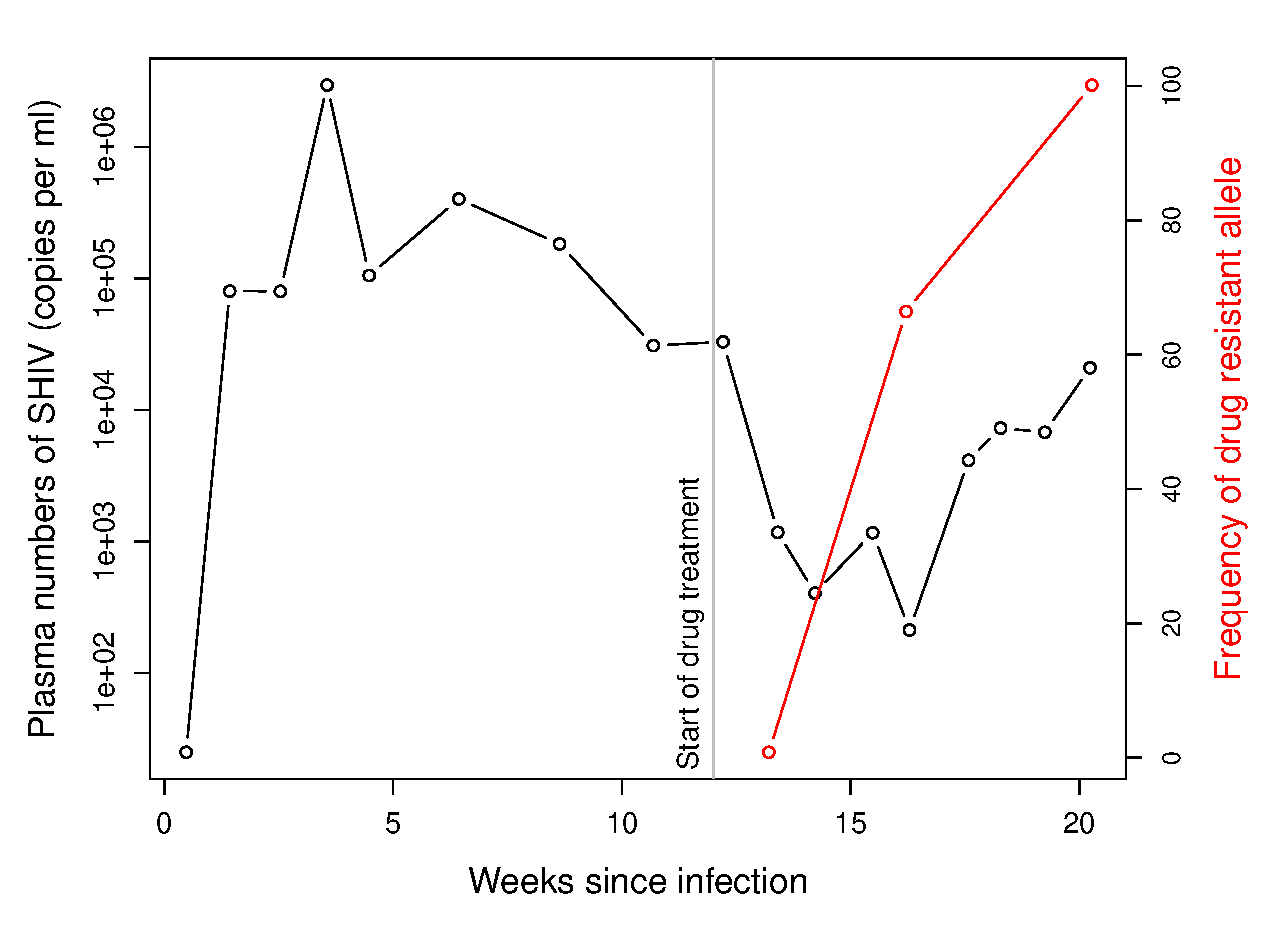
\includegraphics[width= \textwidth]{Journal_figs/single_locus_selection/Feder_HIV/Feder_HIV.pdf}
\end{center}
\caption{The rapid evolution of drug-resistant SHIV. The viral load of
  SHIV in the blood of a macaque (black line), the frequency of a drug
  resistance mutation (red line). Data from \citet{feder2017}. \gitcode{https://github.com/cooplab/popgen-notes/blob/master/Journal_figs/single_locus_selection/Feder_HIV/Feder_HIV.R}} \label{fig:HIV_viral_freqs}
\end{figure}
The rapid spread of this drug-resistant allele through the population is driven by the much greater relative fitness of the drug-resistant allele over the original strain in the presence of the anti-retroviral drug. 

The frequency of allele $A_1$ in the next generation is given by
\begin{equation}
	\label{eq:eq:recHaplMod1}
	p_{t+1} = \frac{P_{t+1}}{P_{t+1} + Q_{t+1}} = \frac{W_1 P_t}{W_1 P_t + W_2 Q_t}
	%= \frac{W_1 (P_t + Q_t)p_t}{W_1 (P_t + Q_t)p_t + W_2 (P_t + Q_t)q_t}
	= \frac{W_1 p_t}{W_1 p_t + W_2 q_t} = \frac{W_1}{\Wbar_t} p_t.
\end{equation}

Importantly, eqn.\ (\ref{eq:eq:recHaplMod1}) tells us that the change in $p$ only depends on a ratio of fitnesses. Therefore, we need to specify fitness only up to an arbitrary constant. As long as we multiply all fitnesses by the same value, that constant will cancel out and eqn.\ (\ref{eq:eq:recHaplMod1}) will hold. Based on this argument, it is very common to scale absolute fitnesses by the absolute fitness of one of the genotypes, e.g.\ the most or the least fit genotype, to obtain relative fitnesses. Here, we will use $w_i$ for the relative fitness of genotype $i$. If we choose to scale by the absolute fitness of genotype $A_1$, we obtain the relative fitnesses $w_1 = W_1/W_1 = 1$ and $w_2 = W_2/W_1$.\\
Without loss of generality, we can therefore rewrite eqn.\ (\ref{eq:eq:recHaplMod1}) as
\begin{equation}
	\label{eq:recHaplMod2}
	p_{t+1} = \frac{w_1}{\wbar} p_t,
\end{equation}
dropping the subscript $t$ for the dependence of the mean fitness on time in our notation, but remembering it.
The change in frequency from one generation to the next is then given by
\begin{equation}
\Delta p_t = p_{t+1} - p_t= \frac{ w_1 p_t}{ \wbar} - p_t = \frac{w_1 p_t - \wbar p_t}{\wbar} = \frac{w_1 p_t - (w_1 p_t + w_2 q_t) p_t}{\wbar} = \frac{w_1 - w_2}{\wbar} p_t q_t,
\label{eq:deltap_haploid}
\end{equation}
recalling that $q_t = 1 - p_t$.\\

Assuming that the fitnesses of the two alleles are constant over time,
the number of the two allelic types $\tau$ generations after time $0$ are
$P_{\tau} = (W_1)^{\tau} P_0$ and $Q_{\tau}=  (W_2)^{\tau} Q_0$, respectively. Therefore, the relative frequency of allele $A_1$ after $\tau$ generations past $t$ is
\begin{equation}
	p_{\tau} = \frac{ (W_1)^{\tau} P_0}{ (W_1)^{\tau} P_0+(W_2)^{\tau} Q_0} = \frac{ (w_1)^{\tau} P_0}{ (w_1)^{\tau} P_0+(w_2)^{\tau} Q_0} = \frac{p_0}{p_0 + (w_2/w_1)^{\tau} q_0},
	\label{eq:haploid_tau_gen}
\end{equation}
where the last step includes dividing the whole term by $(w_1)^{\tau}$ and switching from absolute to relative allele frequencies.
%Rearranging eqn.\ \eqref{eq:haploid_tau_gen} and setting $t = 0$, we can work out the time $\tau$ for the frequency of $A_1$ to change from $p_0$ to $p_{\tau}$. First, we write
%\begin{equation}
%	p_{\tau} = \frac{p_0}{p_0 + (w_2/w_1)^{\tau} q_0}
%\end{equation}
Rearrange this to obtain
\begin{equation}
	\label{eq:estTau}
	\frac{p_{\tau}}{q_{\tau}} = \frac{p_0}{q_0} \left(\frac{w_1}{w_2}\right)^{\tau}.
\end{equation}
Solving this for $\tau$ yields
\begin{equation}
	\label{eq:solTau}
	\tau = \log \left(\frac{p_{\tau} q_0}{q_{\tau} p_0}\right) /  \log\left(  \frac{w_1}{w_2} \right).
\end{equation}
\\

In practice, it is often helpful to parametrize the relative fitnesses $w_i$ in a specific way. For example, we may set $w_1 = 1$ and $w_2 = 1 - s$, where $s$ is called the selection coefficient. Using this parametrization, $s$ is simply the difference in relative fitnesses between the two alleles. Equation \eqref{eq:haploid_tau_gen} becomes
\begin{equation}
	\label{eq:haploid_tau_gen_expl}
	p_{\tau} = \frac{p_{0}}{p_0 + q_0 (1 - s)^{\tau}},
\end{equation}
as $w_2 / w_1 = 1 - s$. Then, if $s \ll 1$, we can approximate $(1-s)^{\tau}$ in the denominator by $\exp(-s\tau)$ to obtain
\begin{equation} \label{eq:haploid_logistic growth}
	p_{\tau} \approx \frac{p_0}{p_0 + q_0 e^{-s\tau}}.
\end{equation}
This equation takes the form of a logistic function. That is because
we are looking at the relative frequencies of two `populations' (of
alleles $A_1$ and $A_2$) that are growing (or declining)
exponentially, under the constraint that $p$ and $q$ always sum to 1. \\

Moreover, eqn.\ \eqref{eq:estTau} for the number of generations $\tau$ it takes for a certain change in frequency to occur becomes
\begin{equation}
	\label{eq:estTauExpl}
	\tau = - \log \left(\frac{p_{\tau} q_0}{q_{\tau} p_0}\right) /  \log\left(1-s\right).
\end{equation}
Assuming again that $s \ll 1$, this simplifies to
\begin{equation}
	\label{eq:estTauExplSimpl}
	\tau \approx \frac{1}{s} \log \left(\frac{p_{\tau} q_0}{q_{\tau} p_0}\right).
\end{equation}


One particular case of interest is the time it takes to go from an absolute
frequency of 1 to near fixation in a population of size $N$.  In this case, we
have $p_0 = 1/N$, and we may set $p_{\tau} = 1 - 1/N$, which is very close to
fixation. Then, plugging these values into eqn.\ \eqref{eq:estTauExplSimpl}, we
obtain

\begin{align}
  \tau &= \frac{1}{s} \log\left( \frac{1 - \nicefrac{2}{N} +
      \nicefrac{1}{N^2}}{\nicefrac{1}{N^2}} \right) \nonumber \\
  &\approx \frac{1}{s} (\log(N) + \log(N-2)) \nonumber \\
  &\approx \frac{2}{s} \log(N)  \label{eq:fixTimeSimpl}
\end{align}
%
where we make the approximations $N^2 - 2N + 1 \approx N^2 - 2N$ and later
$N-2 \approx N$.


\begin{question}
In our example of the evolution of drug resistance, the drug-resistant SHIV virus spread from undetectable frequencies to $\sim 65\%$ frequency by 16 weeks post infection. An estimated effective population size of SHIV is $1.5 \times 10^5$, and its generation time is $\sim 1$ day. Assuming that the mutation arose as a single copy allele very shortly the start of drug treatment at 12 weeks, what is the selection coefficient favouring the drug resistance allele?  
\end{question}




%\begin{question}
%You are studying the frequency of antibiotic-resistant bacteria in a
%patient.  Before administering the antibiotic the frequency of the 
%resistance allele is $\nicefrac{1}{1000}$. You adminster the antibiotic,
%alarming just 8 days later you find the frequency %of the 
%resistance allele to be $99\%$. Assume a generation time of $\nicefrac{1}{4}$ a day for
%these bacteria. \\
%What is the selection coefficient associated with the resistance to antibiotics?
%\end{question}

\paragraph{Haploid model with fluctuating selection}
Selection pressures may change while a polymorphism persists in the population due to environmental changes. 
We can use our haploid model to consider this case where the fitnesses depend on time \citep{Dempster:55}, and
say that $w_{1,t}$ and $w_{2,t}$ are the fitnesses of the two types in
generation $t$. The frequency of allele $A_1$ in generation $t+1$ is
\begin{equation}
p_{t+1} = \frac{w_{1,t}}{\wbar_t} p_t,
\end{equation}
which simply follows from eqn.\ \eqref{eq:recHaplMod2}.
The ratio of the frequency of allele $A_1$ to that of allele $A_2$ in generation $t+1$ is
\begin{equation}
\frac{p_{t+1}}{q_{t+1}} = \frac{w_{1,t}}{w_{2,t}}  \frac{p_{t}}{q_{t}}.
\end{equation}
Therefore, if we think of the two alleles starting in generation $1$ at
frequencies $p_1$ and $q_1$, then $\tau$ generations later,
\begin{equation}
\frac{p_{\tau}}{q_{\tau}} = \left(\prod_{i=1}^{\tau} \frac{w_{1,i}}{w_{2,i}}  \right) \frac{p_{1}}{q_{1}}.
\end{equation}
\\

The question of which allele is increasing or decreasing in frequency comes down
to whether $\left(\prod_{i=1}^{\tau} \nicefrac{w_{1,i}}{w_{2,i}}  \right)$ is
$>1$ or $<1$. As it is a little hard to think about this ratio, we can
instead take the $\tau^{\mathrm{th}}$ root of it and consider
\begin{equation}
\sqrt[\tau]{\left(\prod_{i=1}^{\tau} \frac{w_{1,i}}{w_{2,i}}  \right)} = \frac{\sqrt[\tau]{\prod_{i=1}^{\tau}w_{1,i}}}{\sqrt[\tau]{\prod_{i=1}^{\tau}w_{2,i}}}.
\end{equation}
The term
\begin{equation}
  \sqrt[\tau]{\prod_{i=1}^{\tau}w_{1,i}}  \label{hap_geo_fitness}
\end{equation}
\begin{margintable}
  \begin{tabular}{lcc}
    & $A_1$  & $A_2$\\
    \hline
    Dry & 2 & 1.57 \\
    Wet &  1.16 & 1.57   \\
    \hline
    Arithmetic Mean & 1.58  & 1.57  \\
    Geometric Mean & 1.52 & 1.57 
  \end{tabular}
  \caption{Fitnesses of two alleles in wet and dry years. Means calculated assuming
    equal chances of wet and dry years. The geometric mean is
    calculated as
    $\sqrt{w_{\textrm{wet}}w_{\textrm{dry}}}$. Example numbers
    taken from \citet{seger1987oxford}.} \label{Table:Geom_fitness}
\end{margintable}

is the geometric mean fitness of allele
 $A_1$ over the $\tau$ generations past generation $t$. Therefore, allele $A_1$ will only increase
in frequency if it has a higher geometric mean fitness than allele $A_2$
(at least in our simple deterministic model). This implies that an allele with higher
geometric mean fitness can even invade and spread to fixation if its
(arithmetic) mean fitness is lower than the dominant type.  To see
this consider two alleles that experience the fitnesses given in Table
\ref{Table:Geom_fitness}. The allele $A_1$ does much better in
dry years, but suffers in wet years; while the $A_2$ is generalist and
is not affected by the variable environment. If there is an equal
chance of a year being wet or dry, the $A_1$ allele has
higher (arithmetic) mean fitness, but it will be replaced by the $A_2$
allele as the $A_2$ allele has higher geometric mean fitness (See Figure \ref{fig:haploid_geo}). \\

\begin{figure}
\begin{center}
\includegraphics[width= \textwidth]{figures/Haploid_geom_traj.pdf}
\end{center}
\caption{An example frequency trajectory of the $A_1$ allele under
  variable environments (using the fitnesses from Table
  \ref{Table:Geom_fitness}). Wet years (generations) are shown in red, dry
  years in white. The environment flips at random each year.  Note how the $A_1$ allele increases in frequency in
  the dry years as it has higher fitness, and yet the $A_2$ allele
  still wins out. 
  \gitcode{https://github.com/cooplab/popgen-notes/blob/master/Rcode/Geometric_mean_fitness.R}} \label{fig:haploid_geo}
\end{figure}

\paragraph{Evolution of bet hedging}

%birds nest https://www.biodiversitylibrary.org/ia/Illustrationsne1Jone#page/11/mode/1up
%% great tit nest https://archive.org/stream/britainsbirdsthe00thom/britainsbirdsthe00thom#page/n536/mode/1up
%% blue tit nest https://www.flickr.com/photos/biodivlibrary/6025489801/

%https://twitter.com/rlmcelreath/status/1129013411344453632
Don't put your eggs in one basket, it makes a lot of sense to spread
your bets. Financial advisors often advise you to diversify your
portfolio, rather than placing all your investments in one stock. Even
if that stock looks very strong, you can come a cropper that
$\nicefrac{1}{20}$ times some particular part of the market
crashes. Likewise, evolution can result in risk averse
strategies. Some species of bird lay multiple nests of eggs; some
plants don't put all of their energy into seeds that will germinate next year. It can
even make sense to hedge your bets even if that comes at an average
cost \citep{seger1987oxford}.

To see this lets think more about geometric fitness. We can write the
relative fitness of an allele in a given generation $i$ as $w_{i}= 1+s_i$, such that we can
write your geometric fitness as
\begin{equation}
 \bar{g}= \sqrt[\tau]{\prod_{i=1}^{\tau-1} 1+s_i}  \label{hap_geo_fitness_bh}
  \end{equation}
when we think about products it's often natural to take the $\log$ to
turn it into a sum
\begin{align}
 \log \big( \bar{g} \big) =& \frac{1}{\tau} \sum_{i=1}^{\tau-1} \log \big(1+s_i \big) \nonumber\\
  = & \E \bigg[ \log \big( 1+s_i \big) \bigg]
\end{align}
equating the mean and the expectation. Assuming that $s_i$ is small $\log(1+s_i \big) \approx s_i -
\nicefrac{s_i^2}{2}$, ignoring terms $s_i^3$ and
higher\sidenote{Here we're using a 2nd order Taylor approximation, see
  math appendix eqn \eqref{eqn:Taylor_log_2nd}. } then this is
\begin{align}
  \log \big( \bar{g}  \big) \approx & \E\bigg[  s_i -\nicefrac{s_i^2}{2}  \bigg]  \nonumber\\
  =  & \E \bigg[  s_i \bigg]  - \textrm{var}(s_i)/2 \nonumber\\
\end{align}
\graham{issue with $\E^2(s)$ here}
So genotypes with high arithmetic mean fitness can be selected against,
i.e. have low geometric mean fitness against, if their fitness has too
high a variance across generations \citep{gillespie1973natural,gillespie1977natural}. See our example
above,  Table \ref{Table:Geom_fitness} and Figure \ref{fig:haploid_geo}).

  \begin{marginfigure}
\begin{center}
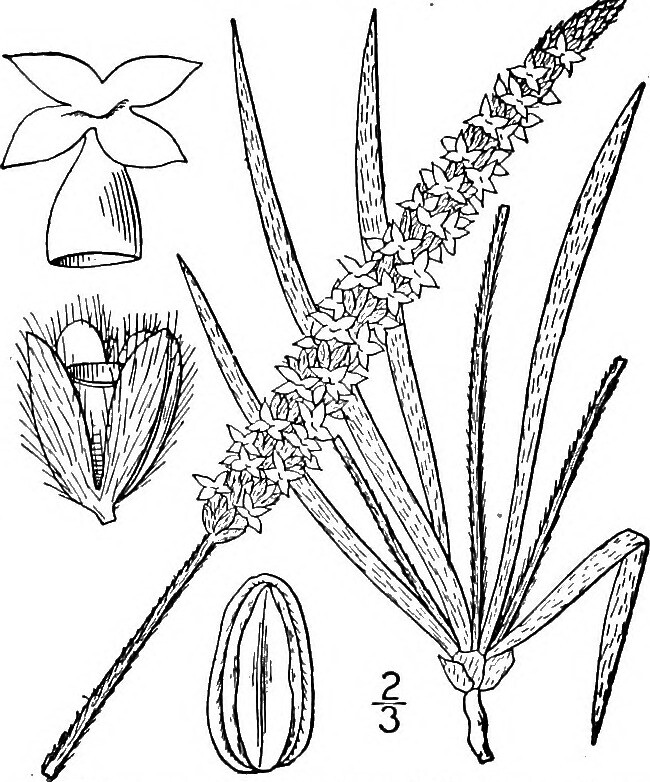
\includegraphics[width= \textwidth]{illustration_images/single_locus_selection/woolly_plantain/20771670485_fb7e476748_b.jpg}
\end{center}
\caption{Woolly plantain ({\it Plantago patagonica}). One of the
  desert annuals shown to have a bet-hedging germination strategy by
  \citet{gremer2014bet}. \BHLNC{An illustrated flora of the northern
    United States, Canada and the British possessions, from
    Newfoundland to the parallel of the southern boundary of Virginia,
    and from the Atlantic Ocean westward to the 102d meridian (1913)  Britton, N.L.}{https://www.flickr.com/photos/internetarchivebookimages/20771670485/}{Cornell University Library}} \label{fig:Woolly_plantain}
\end{marginfigure}

A classic example of bet-hedging is in delayed seed germination in
plants \citep{cohen1966optimizing}. In variable environments, such as
deserts, it may make sense to spread your bets over years by having
only a proportion of your seeds germinate in the first year. However,
delaying germination can come at a cost due to seed
mortality. \citet{gremer2014bet}, using data from a long-term study
various species of Sonoran Desert winter showed that annual plants
were indeed pursuing adaptive bet-hedging strategies.
The plant species with the highest variation in among-year yield had
the lowest germination fraction per year.  Further,
\citeauthor{gremer2014bet} showed through modeling life that by having
per-year germination proportions $<1$ all of the species were
achieving higher geometric fitness at the expense of arithmetic
fitness in the variable desert environment. See Figure
\ref{fig:desert_bet_hedging} for an example of bet hedging in Woolly plantain.

  \begin{figure}
\begin{center}
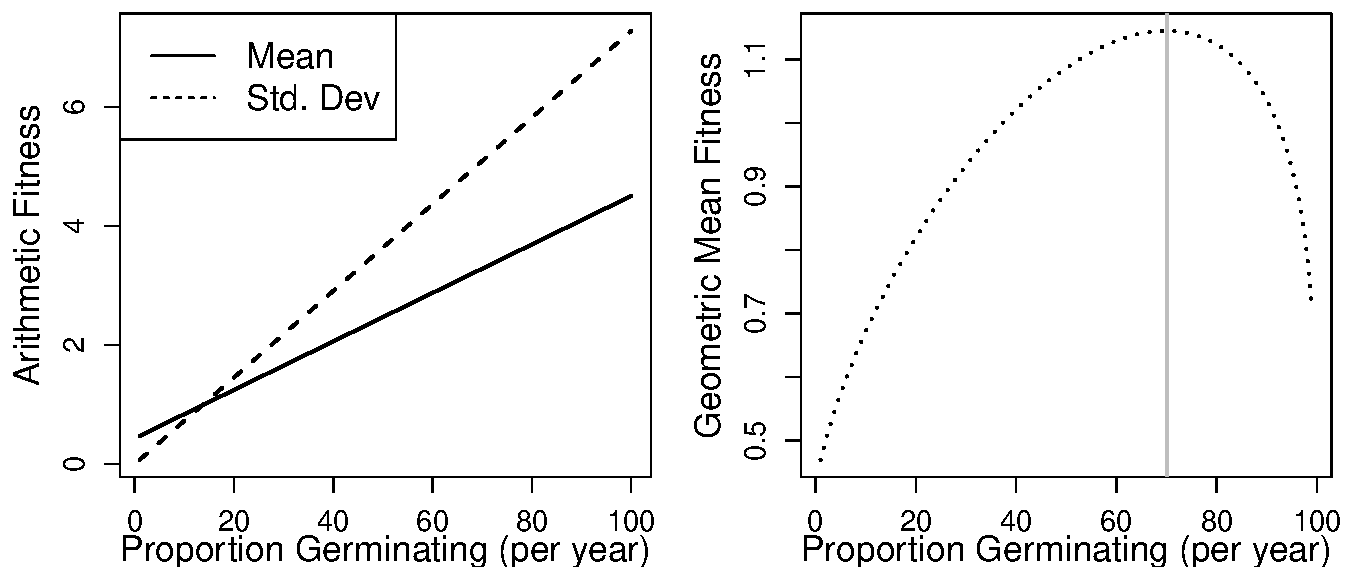
\includegraphics[width= \textwidth]{Journal_figs/single_locus_selection/Gremer_hedging_example/Gremer_hedging_example.pdf}
\end{center}
\caption{  {\it Plantago patagonica}'s arithmetic fitness is an
  increasing function of the proportion of seeds germinating, due to
  seeds not surviving a germination delay. However, the standard
  deviation of fitness also increases with this proportion as they are
  more likely to have all of their seeds germinate in a bad year. Thus
  {\it Plantago patagonica}  can achieve higher geometric fitness by
  only having a proportion of their seeds germinate. Thanks to Jenny
  Gremer for sharing these data from \citet{gremer2014bet}, \gitcode{https://github.com/cooplab/popgen-notes/blob/master/Journal_figs/single_locus_selection/Gremer_hedging_example/Gremer_bet_hedging.R} } \label{fig:desert_bet_hedging}
\end{figure}


%% Gremer seed germination https://onlinelibrary.wiley.com/doi/full/10.1111/ele.12241

%Chicken pox https://www.pnas.org/content/pnas/99/23/15234.full.pdf
Delayed reproduction is also a common example of bet-hedging in
micro-organisms. For example, the Chicken Pox virus, varicella zoster
virus, has a very long latent phase. After it causes chicken pox it enters a latent phase, residing inactive in neurons in
the spinal cord, only to emerge 5-40 years later to cause the disease
shingles. It is hypothesized that the virus actively suppresses itself
as a strategy to allow it to emerge at a later time point as insurance
against there being no further susceptible hosts at the time of its
first infection \citep{stumpf2002herpes}. 

% https://eebweb.arizona.edu/faculty/venable/pdfs/Gremer&Venable2014.pdf
%experimental evolution of bet-hedging http://www.indiana.edu/~curtweb/L567/readings/bet%20hedging%20evolution.pdf

\graham{NOTE about how haploid model can be useful for thinking about
  ESS }

\begin{figure}
\begin{center}
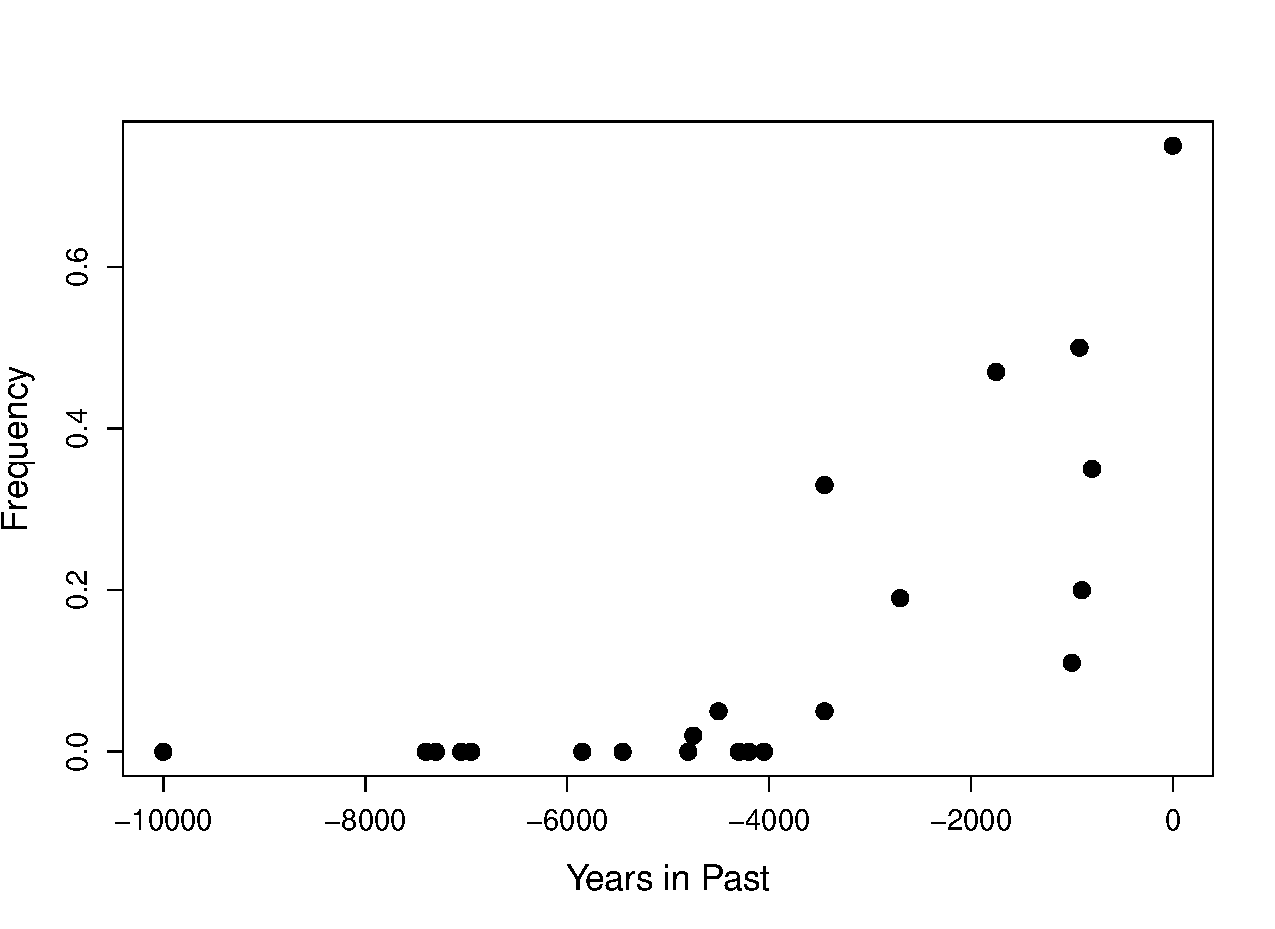
\includegraphics[width= \textwidth]{Rcode/Lactase_example/Lactase_freq_time.pdf}
\end{center}
\caption{Frequency of the Lactase persistence allele in ancient and
  modern samples form Central Europe. Data compiled by
  \citet{marciniak2017} from various sources. Thanks to Stephanie
  Marciniak for sharing these data. \gitcode{https://github.com/cooplab/popgen-notes/blob/master/Rcode/Lactase_example/Lactase_plots.R}} \label{fig:LCT_freqs}
\end{figure}

\subsection{Diploid model}

\begin{marginfigure}
\begin{center}
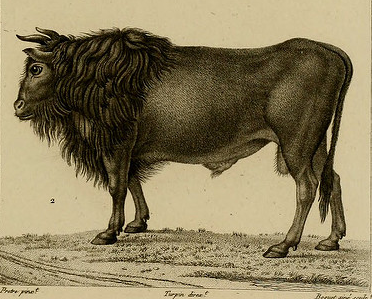
\includegraphics[width= \textwidth]{illustration_images/single_locus_selection/cow_auroch/auroch.png}
\end{center}
\caption{Auroch ({\it Bos primigenius}). Aurochs are an extinct species of large wild cattle that cows
  were domesticated from. \IANC{Dictionnaire des sciences naturelles. 1816 Cuvier,
  F.G. }{https://www.flickr.com/photos/internetarchivebookimages/20713828960/in/photolist-owtfpr-owkoQN-obMTQg-owc9mc-rgpdRz-otq59G-oeZFD1-ottAnF-otuXhK-odKHJY-oqYxSb-oviGuD-ytox4c-owa3cJ-yc73Ji-wtrahu-ouf1fo-wXHoQ6-t97h27-owfa8h-xisfNf-waBt8s-x8859A-xwY4eG-wpCm8P-oev6vL-oy1AhH-tNJj8g-xGgALJ-x2kj8g-xDphGC-oxvRgt-x8eFQp-xypMG5-wKqr2k-xnCp1u-xpC2zS-wt5Lpp-xUjHhG-wGJBAQ-wv5dnr-xqLVc3-wPhru1}{NCSU Libraries}} \label{fig:auroch}
\end{marginfigure}

We will now move on to a diploid model of a single locus with two segregating alleles. As an example of the change in the frequency of an allele driven by selection, lets consider the evolution of Lactase persistence. A number of different human populations that historically have raised cattle have convergently evolved to maintain the expression of the protein Lactase into adulthood (in most mammals the protein is switched off after childhood), with different lactase-persistence mutations having arisen and spread in different pastoral human populations. 
This continued expression of Lactase allows adults to break down Lactose, the main carbohydrate in milk, and so benefit nutritionally from milk-drinking. This seems to have offered a strong fitness benefit to individuals in pastoral populations. 

With the advent of techniques to sequence ancient human DNA, researchers can now potentially track the frequency of selected mutations over thousands of years. The frequency of a Lactase persistence allele in ancient Central European populations is shown in Figure \ref{fig:LCT_freqs}. The allele is absent more than 5,000 years ago, but now found at frequency of upward of $70\%$ in many European populations. 


We will assume that the difference in fitness between the three
genotypes comes from differences in viability, i.e.\ differential
survival of individuals from the formation of zygotes to reproduction.  
We denote the absolute fitnesses of genotypes $A_1A_1$, $A_1A_2$, and $A_2A_2$ by $W_{11}$, $W_{12}$, and $W_{22}$. Specifically, $W_{ij}$ is the probability that a zygote of genotype $A_iA_j$ survives to reproduction.
Assuming that individuals mate at random, the number of zygotes that are of the three genotypes and form generation $t$ are
\begin{equation}
Np_t^2, ~~~  N2p_tq_t, ~~~ Nq_t^2.
\end{equation}

The mean fitness of the population of zygotes is then
\begin{equation}
	\Wbar_t = W_{11} p_t^2+W_{12} 2p_tq_t  +  W_{22} q_t^2.
\end{equation}
Again, this is simply the weighted mean of the genotypic fitnesses.
\\

How many zygotes of each of the three genotypes survive to reproduce? \erin{plot needs caption and title}
An individual of genotype $A_1A_1$ has a probability of $W_{11}$ of
surviving to reproduce, and similarly for other genotypes. Therefore, the expected number of $A_1A_1$, $A_1A_2$, and $A_2A_2$ individuals who survive to reproduce is
\begin{equation}
	NW_{11} p_t^2, ~~~ NW_{12} 2p_tq_t , ~~~ N W_{22} q_t^2.
\end{equation}
It then follows that the total number of individuals who survive to
reproduce is
\begin{equation}
	N \left(W_{11} p_t^2+W_{12} 2p_tq_t  +  W_{22} q_t^2 \right).
\end{equation}
This is simply the mean fitness of the population multiplied by the
population size (i.e.\ $N \wbar$).\\

The relative frequency of $A_1A_1$ individuals at reproduction
is simply the number of $A_1A_1$ genotype individuals at reproduction ($NW_{11} p_t^2$)
divided by the total number of individuals who survive to reproduce
($N \Wbar$), and likewise for the other two genotypes.
Therefore, the relative frequency of individuals with the three different genotypes at reproduction is
\begin{equation}
	\frac{NW_{11} p_t^2}{N\Wbar}, ~~~ \frac{NW_{12} 2p_tq_t}{N\Wbar} , ~~~ \frac{N W_{22} q_t^2}{N\Wbar}
\end{equation}
(see Table \ref{dip_fitness_table}).\\

\begin{table*}
\begin{center}
\begin{tabular}{lccc}
\hline
& $A_1A_1$ & $A_1A_2$ & $A_2A_2$\\
\hline
Absolute no. at birth & $Np_t^2$ & $N2p_tq_t$ & $Nq_t^2$\\
Fitnesses & $W_{11}$ & $W_{12}$& $W_{22}$\\
Absolute no.\ at reproduction & $NW_{11} p_t^2$ & $NW_{12} 2p_tq_t$& $N W_{22} q_t^2$\\
Relative freq.\ at reproduction & $ \frac{W_{11}}{\Wbar} p_{t}^2$ & $ \frac{W_{12}}{\Wbar} 2 p_{t} q_{t}$ & $\frac{W_{22}}{\Wbar} q_{t}^2$\\
\end{tabular}
\end{center}
\caption{Relative genotype frequencies after one episode of viability selection.} \label{dip_fitness_table}
\end{table*}

%\gc{Dobzhansky}

%\begin{center}
%\begin{tabular}{lccc}
%\hline
% & ST/ST & ST/CH & CH/CH \\  ##From Evolution encylopedia
%Eggs & 41 & 82 &27\\
%Adults & 25 & 74 & 12\\
%\end{tabular}
%\end{center}

As there is no difference in the fecundity of the three genotypes, the
allele frequencies in the zygotes forming the next generation are simply the
allele frequency among the reproducing individuals of the previous generation. Hence, the frequency of $A_1$ in generation $t+1$ is
\begin{equation}
	p_{t+1} = \frac{W_{11} p_t^2 + W_{12} p_tq_t}{\Wbar}
	\label{pgen_dip}.
\end{equation}
\erin{it might help students understand this equation more to mention here that the expected 2 in 2pq is being cancelled out by the 1/2 for only one A1 allele in hets...or to just include that step though it's fairly trivial} Note that, again, the absolute value of the fitnesses is irrelevant to
the frequency of the allele. Therefore, we can just as easily replace
the absolute fitnesses with the relative fitnesses. That is, we may replace $W_{ij}$ by $w_{ij} = W_{ij}/W_{11}$, for instance. \\

Each of our genotype frequencies is responding to selection in a
manner that depends just on its fitness compared to the mean fitness
of the population. For example, the frequency of the $A_1A_1$ homozygotes
increases from birth to adulthood in proportion to $\nicefrac{W_{11}}{\Wbar}$. In
fact, we can estimate this fitness ratio for each genotype by comparing
the frequency at birth compared to adults. As an example of this calculation, we'll
look at some data from sticklebacks. 
\begin{marginfigure}
\begin{center}
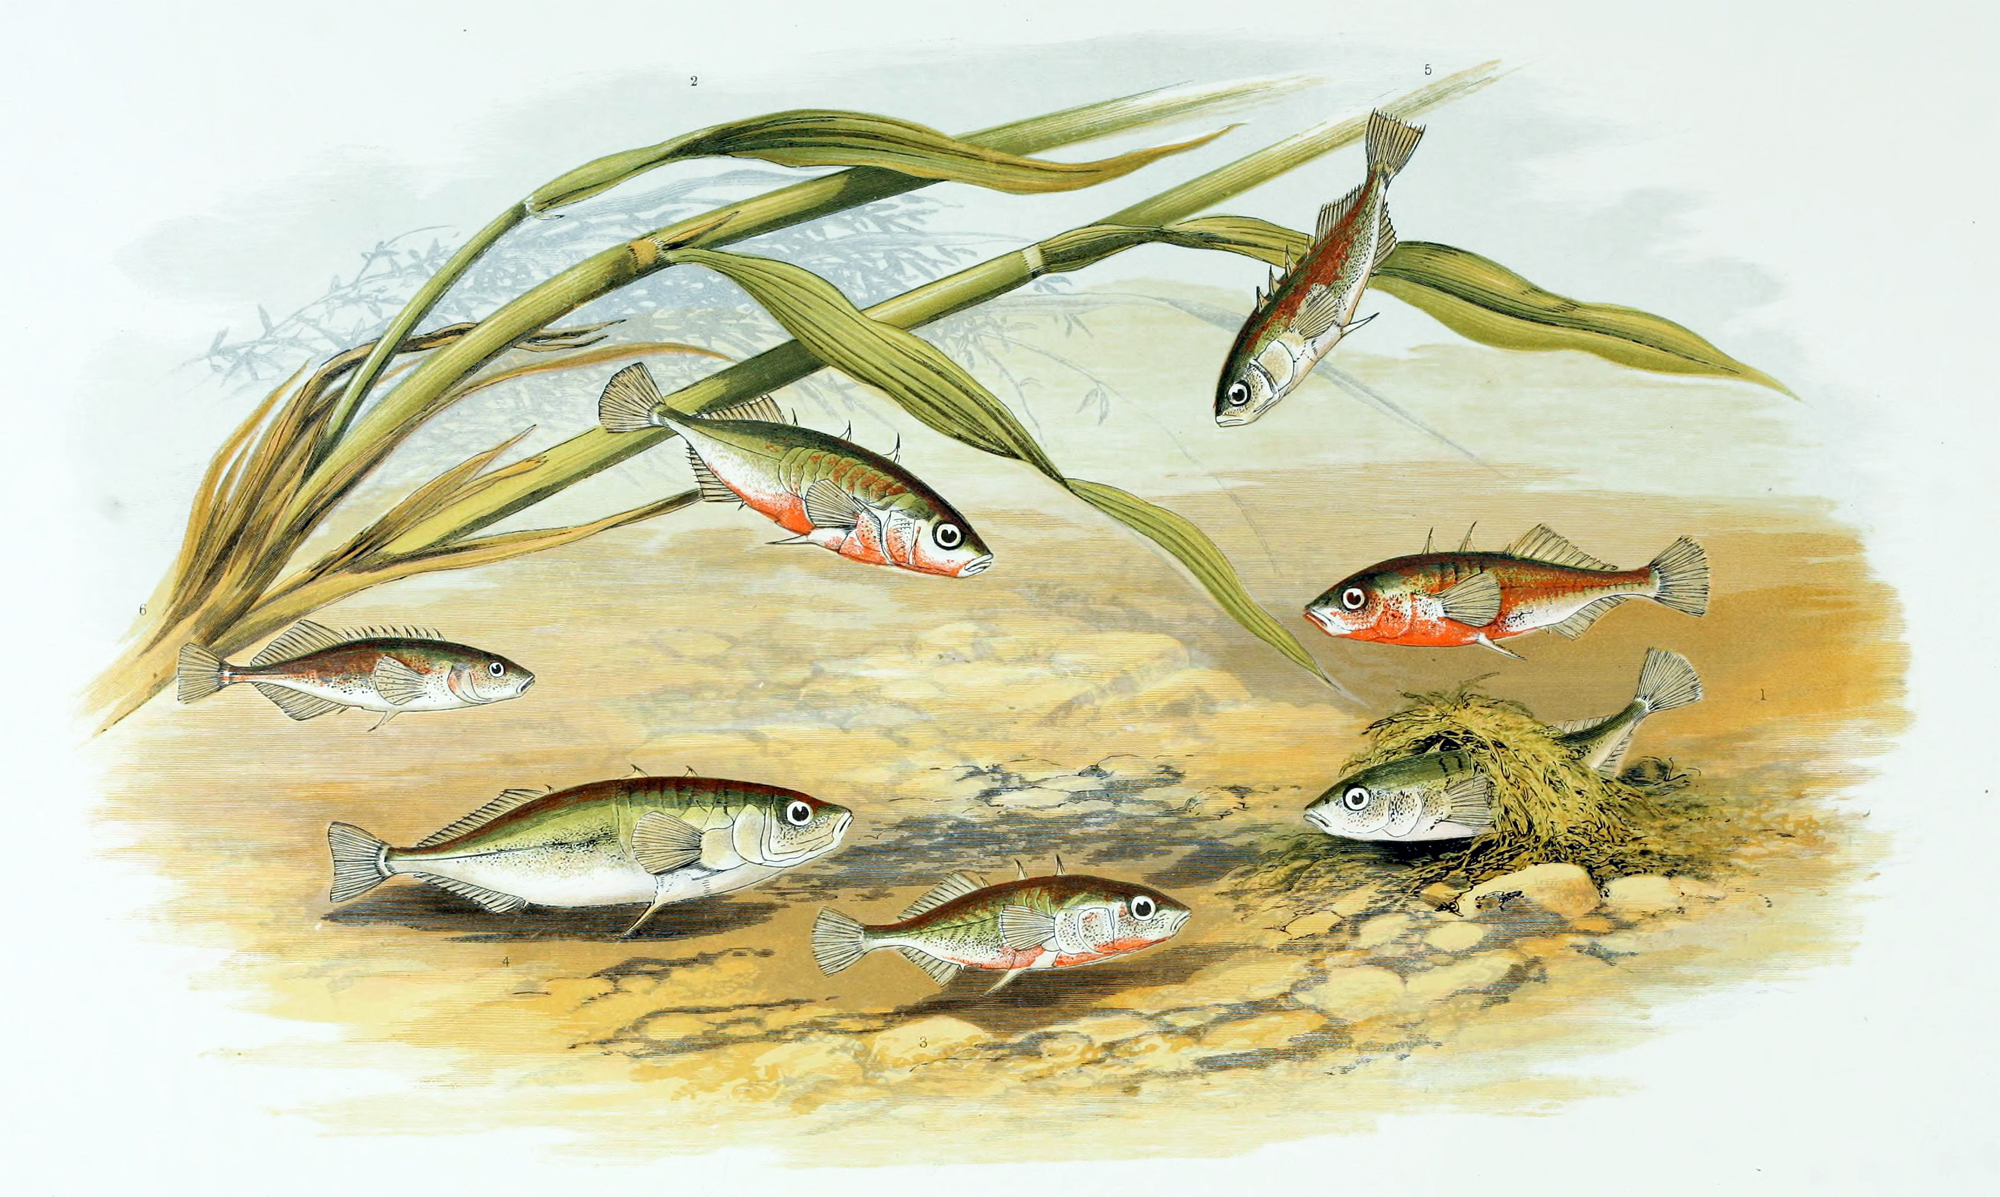
\includegraphics[width= 1.2 \textwidth]{illustration_images/single_locus_selection/Stickleback/Gasterosteus_aculeatus_1879.jpg}
\end{center}
\caption{Freshwater threespine Stickleback ({\it
    G. aculeatus}). \BHLNC{British fresh-water fishes. Houghton W
    1879.}{https://commons.wikimedia.org/wiki/File:Gasterosteus_aculeatus_1879.jpg}{Ernst
    Mayr Library, Harvard.}} \label{fig:stickleback}
\end{marginfigure}
Marine threespine stickleback ({\it Gasterosteus aculeatus})
independently colonized and adapted to many freshwater lakes
as glaciers receded following the last ice age, making sticklebacks a wonderful system for studying the genetics of adaptation. In marine habitats, most of the stickleback have armour plates to protect them
from predation, but freshwater populations repeatedly evolve the
loss of armour plates due to selection on an allele at the
Ectodysplasin gene (EDA).  This allele is found as a standing variant at very low frequency marine populations;
\citet{Barrett:08} took advantage of this fact and collected and bred
a population of marine individuals carrying both the low- (L) and
completely- plated (C) alleles. They introduced the offspring of this
cross into four freshwater ponds and monitored genotype frequencies
\sidenote{The actual dynamics observed by \citeauthor{Barrett:08} are more complicated as in the very young fish selection reverses direction.}
over their life courses: 
\begin{center}
\begin{tabular}{lccc}
 & CC & LC & LL \\
Juveniles & 0.55 & 0.23 & 0.22\\
Adults     & 0.21 & 0.53 & 0.26\\
Adults/Juv. ($W_{\bullet}/\Wbar$)  & 0.4 & 2.3 & 1.2 \\
rel. fitness ($W_{\bullet}/W_{12}$)  & 0.17 & 1.0 & 0.54 \\
\end{tabular}
\end{center}
\erin{I changed the fitness calculated above in the 3rd row to being labelled Adults/Juv. not Juv./Adult unfortunately after notes were distributed to class} The heterozygotes have increased in frequency dramatically in the
population as their fitness is more than double the mean fitness of
the population. We can also calculate the relative fitness of each
genotype by dividing through by the fitness of the fittest genotype,
the heterozygote in this case (doing this cancels through
$\Wbar$). The relative fitness of the $CC$ is $\sim 1/5$ of the
heterozygote. Note that this calculation does not rely on the genotype frequencies being at their HWE in the juveniles.

\begin{question}
{\bf A)} What is the frequency of the low-plated EDA allele ($L$) at the start of the stickleback experiment? \\
{\bf B)} What is the frequency in the adults? \\
{\bf C)} Also calculate the frequency in adults using the relative
fitnesses. 
\end{question}




The change in frequency from generation $t$ to $t+1$ is
\begin{equation}
\Delta p_t = p_{t+1} -p_{t}= \frac{w_{11} p_t^2 + w_{12} p_tq_t}{\wbar} - p_t. \label{deltap_dip1}
\end{equation}
To simplify this equation, we will first define two variables $\wbar_1$ and $\wbar_2$ as
\begin{eqnarray}
	\wbar_1 & = w_{11} p_t + w_{12} q_t, \\
	\wbar_2 & =  w_{12} p_t+ w_{22} q_t.
\end{eqnarray}
\graham{Comment that these are the additive effects of our alleles}
These are called the marginal fitnesses of allele $A_1$
and $A_2$, respectively. They are so called as $\wbar_1$ is the
average fitness of an allele $A_1$, i.e.\ the fitness of $A_1$ in a
homozygote weighted by the probability it is in a homozygote ($p_t$)
plus the fitness of $A_1$ in a
heterozygote weighted by the probability it is in a heterozygote ($q_t$).
We further note that the mean relative fitness can be expressed in terms of the marginal fitnesses as
\begin{equation}
	\label{eq:meanFitInTermsOfMargFit}
	\wbar = \wbar_1 p_t + \wbar_2 q_t,
\end{equation}
where, for notational simplicity, we have omitted subscript t for the dependence of mean and marginal fitnesses on time.\\

We can then rewrite eqn.\ \eqref{deltap_dip1} using $\wbar_1$ and $\wbar_2$ as
\begin{equation}
	\Delta p_t = \frac{ (\wbar_1-\wbar_2)}{\wbar} p_t q_t.
	\label{deltap_dip2}
\end{equation}
The sign of $\Delta p_t$, i.e. whether allele $A_1$ increases of decreases
in frequency, depends only on the sign of $(\wbar_1-\wbar_2)$.
The frequency of $A_1$ will keep increasing over the generations so
long as its marginal fitness is higher than that of $A_2$,
i.e.\ $\wbar_1 > \wbar_2$, while if $\wbar_1 < \wbar_2$, the
frequency of $A_1$ will decrease. Note the similarity between eqn.\ \eqref{deltap_dip2} and the respective expression for the haploid model in eqn.\ \eqref{eq:deltap_haploid}. (We will return to the
special case where $\wbar_1 = \wbar_2$ shortly).\\

We can also rewrite \eqref{deltap_dip1} as
\begin{equation}
\Delta p_t =\frac{1}{2} \frac{p_tq_t}{\wbar} \frac{d \wbar}{dp}, 
\label{deltap_dip3}
\end{equation}
\marginnote{To see this we can write
\begin{align*}
  \frac{d\bar{w}}{dp} &= \frac{d}{dp} \left( W_{11} p^2 + 2 W_{12} p \right. \nonumber\\
   & ~~ \left. - 2 W_{12} p^2 + W_{22} -  2 W_{22} p +  W_{22} p^2\right) \nonumber\\
  &= 2\left(w_{11} p + w_{12} - 2pw_{12} - w_{22} - w_{22} + w_{22} p\right)
\end{align*}
On expansion of $\bar{w}_1 - \bar{w}_2$, we see that it matched the terms in
the parentheses in the expression above. Thus, we see that we can replace
$\bar{w}_1 - \bar{w}_2$ with $\nicefrac{1}{2} \frac{d\bar{w}}{dp}$.
}

This form shows that the frequency of $A_1$ will increase ($\Delta p_t > 0$) if the mean fitness is an increasing function of the frequency of $A_1$ (i.e.\ if $\frac{d \wbar}{dp}>0$). On the other hand, the frequency of $A_1$ will decrease ($\Delta p_t < 0$) if the mean fitness is a decreasing function of the frequency of $A_1$ (i.e.\ if $\frac{d \wbar}{dp}<0$).
%This form shows that
%$\Delta p_t$ in increase if $\frac{d \wbar}{dp}>1$, i.e. increasing the
%frequency of $1$ increases the mean fitness, while the frequency of
%the allele with decrease if this increases the mean fitness of the
%population ($\frac{d \wbar}{dp}>1$).
Thus, although selection acts on
individuals, under this simple model, selection is acting to increase
the mean fitness of the population. The rate of this increase is proportional to
the variance in allele frequencies within the population
($p_tq_t$). This formulation suggested to \citet{wright1932} the view of natural
selection as moving populations up local fitness peaks, as we
encountered in Section \ref{section:pheno_fitness_landscapes} in
discussing phenotypic fitness peaks. Again this view of selection as
maximizing mean fitness only holds true
if the genotypic fitnesses are frequency independent, later in this
chapter we'll discuss some important cases where that doesn't hold. \\

%\begin{question}
%Show that eqns.\ \eqref{deltap_dip3} and \eqref{deltap_dip2} are
%equivalent. (Trickier question.)\\
%\end{question}

\begin{question}
For many generations you have been studying an annual wildflower that has two color morphs, orange and white. You have discovered that a single bi-allelic locus controls flower color, with the white allele being recessive. The pollinator of these plants is an almost blind bat, so individuals are pollinated at random with respect to flower color. Your population census of 200 individuals showed that the population consisted of 168 orange-flowered individuals, and 32 white-flowered individuals.\\
Heavy February rainfall creates optimal growing conditions for an
exotic herbivorous beetle with a preference for orange-flowered
individuals.  This year it arrives at your study site with a ravenous
appetite.  Only 50\% of orange-flowered individuals survive its wrath,
while 90\% of white-flowered individuals survive until the end of the
growing season.  \\
%Additionally, surviving orange flowered individuals produce 80 seeds on average, while surviving white-flowered individuals produce 100 seeds on average. 
{\bf A)} What is the initial frequency of the white allele, and what do you
have to assume to obtain this?\\
{\bf B)} What is the frequency of the white allele in the seeds forming the next generation?\\
\end{question}


%%Selection coeffs in diploid model
\subsection{Diploid directional selection}
So far, our treatment of the diploid model of selection has been in terms of generic fitnesses $w_{ij}$. In the following, we will use particular parameterizations to gain insight about two specific modes of selection: directional selection and heterozygote advantage.

Directional selection means that one of the two alleles always has higher marginal fitness than the other one. Let us assume that $A_1$ is the fitter allele, so that $w_{11} \geq w_{12} \geq w_{22}$, and hence $\wbar_1 > \wbar_2$. As we are interested in changes in allele frequencies, we \sa{may use} relative fitnesses. We parameterize the reduction in relative fitness in terms of a selection coefficient, similar to the
one we met in the haploid selection section, as follows:\\
\begin{center}
\begin{tabular}{lccc}
genotype & $A_1A_1$ & $A_1A_2$ & $A_2A_2$ \\
absolute fitness & $W_{11}$ & $ \geq W_{12} \geq$ & $W_{22}$ \\
relative fitness (generic) & $w_{11} = W_{11}/W_{11}$ & $w_{12} = W_{12}/W_{11}$ & $w_{22} = W_{22}/W_{11}$ \\
relative fitness  (specific) & $1$ & $1-sh$ & $1-s$. \\
\end{tabular}\\
\end{center}
Here, the selection coefficient $s$ is the difference in relative
fitness between the two homozygotes, and $h$ is the
dominance coefficient. \sa{For selection to be directional, we require that $0 \leq h \leq 1$ holds. The dominance coefficient allows us to move between two extremes. One is when $h = 0$, such that allele $A_1$ is fully dominant and $A_2$ fully recessive. In this case, the heterozygote $A_1A_2$ is as fit as the $A_1A_1$ homozgyote genotype. The inverse holds when $h = 1$, such that allele $A_1$ is fully recessive and $A_2$ fully dominant.}\\

\begin{marginfigure}
\begin{center}
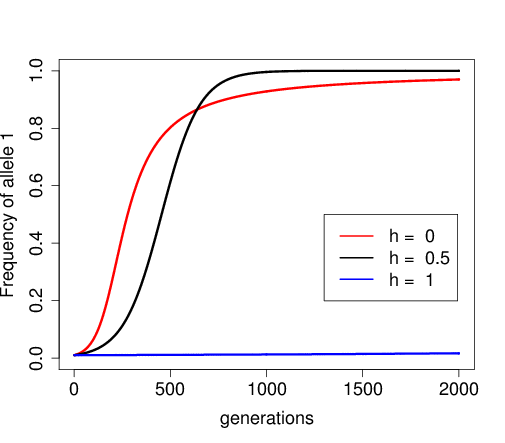
\includegraphics[width=1.2 \textwidth]{figures/simple_diploid_trajs.png}
\end{center}
\caption{The trajectory of the frequency of allele $A_1$, starting
  from $p_{0}=0.01$, for a selection coefficient $s=0.01$ and three
  different dominance coefficients. The recessive beneficial allele ($h=1$) will
  eventually fix in the population, but it takes a long
  time. \gitcode{https://github.com/cooplab/popgen-notes/blob/master/Rcode/diploid_sel.R}}
  \label{fig:diploid_traj}
\end{marginfigure}

%\gc{Yellow monkey flowers ({\it Mimulus guttatus}) have repeatedly adapted
%to the toxic soils found at copper mines throughout the Californian
%foothills in the past 150 years. Kevin Wright   }



%, of the $12$ and
%$22$ genotypes we will use selection coefficients $s_{12} \leq 0$ and
%$s_{22} \leq s_{12}$

We can then rewrite eqn.\ \eqref{deltap_dip2} as
\begin{equation}
\Delta p_t = \frac{p_ths + q_t s(1-h)}{\wbar}p_tq_t ,
\label{deltap_direct}
\end{equation}
where
\begin{equation}
\wbar = 1-2p_tq_t sh-q_t^2s.
\end{equation}\\

\begin{question}
Throughout the Californian foothills are old copper and gold-mines, which have dumped out soils that are polluted with heavy metals. While these toxic mine tailing are often depauperate of plants,  {\it Mimulus guttatus} and a number of other plant species have managed to adapt to these harsh soils. \citet{wright2015adaptation} have mapped one of the major loci contributing to the adaptation to soils at two mines near Copperopolis, CA. \citeauthor{wright2015adaptation} planted homozygote seedlings out in the mine tailings and found that only $10\%$ of the homozygotes for the non-copper-tolerant allele survived to flower, while $40\%$ of the copper-tolerant seedlings survived to flower.\\

\begin{marginfigure}
\begin{center}
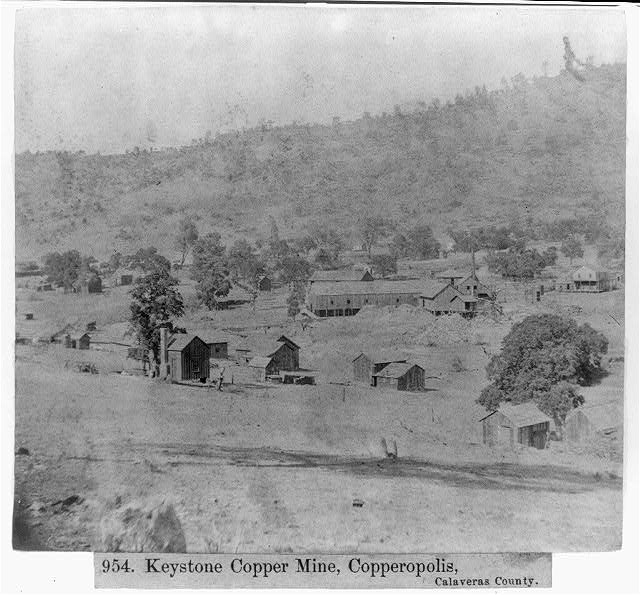
\includegraphics[width = 1.2 \textwidth]{illustration_images/single_locus_selection/Copperopolis/KeystoneCopperMineCopperopolisCalaverasCounty.jpg}
\end{center}
\caption{Keystone Copper Mine 1866, Copperopolis, Calaveras
  County. \newline \noindent \tiny{ Image from
  \href{https://picryl.com/media/keystone-copper-mine-copperopolis-calaveras-county}{picryl}.
Source Library of Congress, Public Domain. }}
  \label{fig:Copperopolis}
\end{marginfigure}

{\bf A)} What is the selection coefficient acting against the non-copper-tolerant allele on the mine tailing?\\
{\bf B)} The copper-tolerant allele is fairly dominant in its action on fitness. If we assume that $h=0.1$, what percentage of heterozygotes should survive to flower?
\end{question}
\begin{question}
Comparing the red ($h=0$) and black ($h=0.5$) trajectories in Figure \ref{fig:diploid_traj}, provide an explanation for why $A_1$ increases faster initially if $h=0$, but then approaches fixation more slowly compared to the case of $h=0.5$.
\end{question}

%%%% Another possible fox image
%%%  https://twitter.com/BioDivLibrary/status/1046777289416081408

%%%%%%%%%%%%%%%%%%%%%FOXSES

\begin{figure}
\begin{center}
  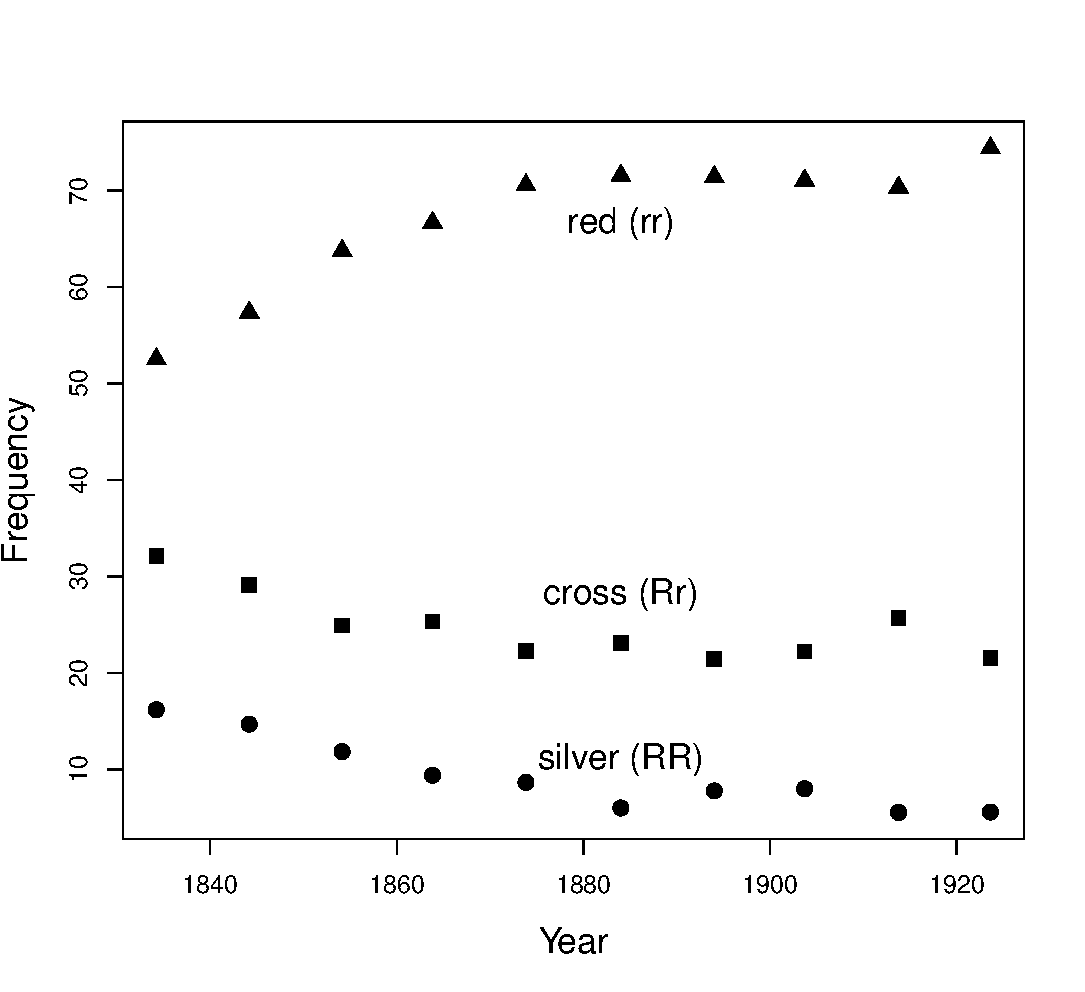
\includegraphics[width = 0.8 \textwidth]{Journal_figs/single_locus_selection/silver_fox/fox_morph_freqs.pdf}
\end{center}
\caption[][3cm]{The frequency of red, cross, and silver fox morphs over the
  decades in Eastern Canada. These data are well described by
  recessive selection acting against the silver fox morph. Data from
  \citet{elton:42}, compiled by \citet{Allendorf:09}. \gitcode{https://github.com/cooplab/popgen-notes/blob/master/Journal_figs/single_locus_selection/silver_fox/fox_morphs.R}} \label{fig:Fox_morph_freqs}
\end{figure}
To see how dominance affects the trajectory of a real
polymorphism, we'll consider an example from a colour polymorphism in
red foxes ({\it Vulpes vulpes}). \begin{marginfigure}\begin{center}
  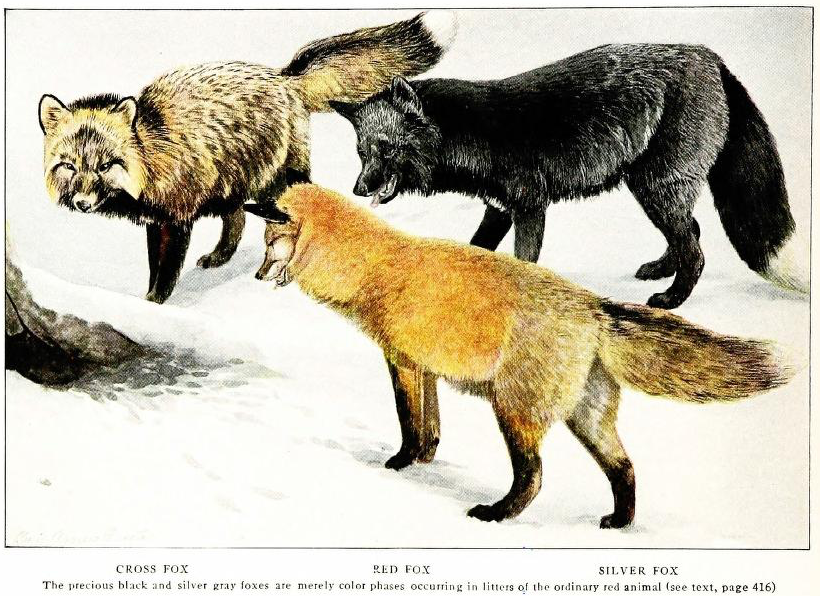
\includegraphics[width = \textwidth]{illustration_images/single_locus_selection/fox_morphs/fox_morphs_silver_cross.png}
\end{center}
\caption{Three colour morphs in red fox {\it V. vulpes}, cross, red,
  and silver foxes from left to right. \BHLNKC{The larger North American
    mammals" Nelson, E.W., Fuertes,
    L.A. 1916.}{https://www.flickr.com/photos/internetarchivebookimages/20578302420/in/photolist-wZ1CDZ-x4aTMj-tCTNnY-sFEbZG-xphfQ3-xmrbnA-xiXcDj-xejHVF-xtiB5G-xbxj1h-xsQdrP-wvPad5-xsFHvi-xqbZ1n-wsJA56-wrzbGj-xhvUJC-xgyia4-wYQ2pR-wXZf6j-wiuZ1t-wWKbS1-whsqaP-whio1h-xeiFTH-wWNQYe-xeiq1a-xdwa1s-wQExt6-x8BrsK-wPgGBE-w9DN9W-x75ojD-wP27dM-w9D6Ye-x6tXdt-wNRKTC-w9AXfX-x5rdVc-x25Puc-vvxmtP-tJ16gt-tAVz57-tmv9Zh-tCXVo2-owo4PL-oum6R1-oeCRWg-oeg5dH-ot9SVz}{Cornell University Library}} \label{fig:Fox_morphs}
\end{marginfigure}  There are three colour morphs of red foxes: silver, cross, and
red (see Figure \ref{fig:Fox_morphs}), with this difference primarily
controlled by a single polymorphism with genotypes RR, Rr, and rr respectively. The fur pelts of the silver morph
fetched three times the price for hunters compared to cross (a smoky red) and red
pelts, the latter two being seen as roughly equivalent in worth. Thus
the desirability of the pelts acts as a recessive trait, with much
stronger selection against the silver homozygotes.  As a
result of this price difference, silver foxes were hunted more
intensely and declined as a proportion of the population in Eastern Canada, see Figure
\ref{fig:Fox_morph_freqs}, as documented by \citeauthor{elton:42},
from $16\%$ to $5\%$ from 1834 to 1937.
\citeauthor{haldane:42} reanalyzed these data and showed that they
were consistent with recessive selection acting against the silver
morph alone. 
Note how the heterozygotes (cross) decline somewhat as a
result of selection on the silver homozygotes, but overall the R
allele is slow to respond to selection as it is `hidden' from
selection in the heterozygote state.

\graham{Add selection lines or get students to do that as an exercise.}


%%dominant colour poly in owls
%%https://www.ncbi.nlm.nih.gov/pmc/articles/PMC3105316/

\paragraph{Directional selection on an additive allele.}
A special case is when $h = 0.5$. This case is the case of no dominance, as the interaction among alleles with respect to fitness is strictly additive. Then, eqn.\ \eqref{deltap_direct} simplifies to
\begin{equation}
	\Delta p_t = \frac{1}{2}\frac{s}{\wbar}p_tq_t .
	\label{deltap_add}
\end{equation}


If selection is very weak, i.e.\ $s \ll 1$, the denominator ($\wbar$) is close to $1$ and we have
\begin{equation}
	\Delta p_t = \frac{1}{2} s p_t q_t .
	\label{deltap_add_simpl}
\end{equation}
It is instructive to compare eqn.\ \eqref{deltap_add_simpl} to the respective expression under the haploid model. To this purpose, start from the generic term for $\Delta p_t$ under the haploid model in eqn.\ \eqref{eq:deltap_haploid} and set $w_1 = 1$ and $w_2 = 1-s$. Again, assume that $s$ is small, so that eqn.\ \eqref{eq:deltap_haploid} becomes $\Delta p_t = s p_t q_t$. Hence, if $s$ is small, the diploid model of directional selection without dominance is identical to the haploid model, up to a factor of $1/2$. That factor is due to the choice of the parametrisation; we could have set $w_{11} = 1$, $w_{12} = 1-s$, and $w_{22} = 1-2s$ in our diploid model instead, in which case the agreement with the haploid model would be perfect.\\

From this analogy, we can borrow some insight we gained from the
haploid model. Specifically, the trajectory of the frequency of allele
$A_1$ in the diploid model without dominance follows a logistic growth
curve similar to eqn. \eqref{eq:haploid_logistic growth}. From this similarity, we can extrapolate from Equation \eqref{eq:estTauExplSimpl} to find the time it takes for our diploid, beneficial, additive allele ($A_1$) to move from frequency $p_0$ to $p_{\tau}$:
\begin{equation}
	\tau \approx \frac{2}{s} \log \left(\frac{p_{\tau} q_0}{q_{\tau} p_0}\right)
\end{equation}
generations; this just differs by a factor of $2$ from our haploid model. Using this result we can find the time it takes for our favourable, additive allele ($A_1$) to transit from its entry into the population ($p_0 =1/(2N)$)
to close to fixation ($p_{\tau} =1-1/(2N)$):
\begin{equation}
	\tau \approx \frac{4}{s} \log(2N)  \label{eq:diploid_fix_time}
\end{equation}
generations. Note the similarity to eqn.\ \ref{eq:fixTimeSimpl} for the haploid model, with a difference
by a factor of 2 due to the choice of parametrization 
(and that the number of alleles is $2N$ in the diploid model, rather than $N$). Doubling our selection coefficient halves the time it takes for our allele to move through the population.\\


% https://www.flickr.com/photos/internetarchivebookimages/17578330873/
\begin{marginfigure}
\begin{center}
  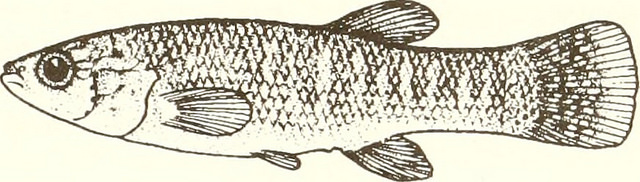
\includegraphics[width = \textwidth]{illustration_images/single_locus_selection/killifish/20974603315_1f9775189e_z.jpg}
\end{center}
\caption{Gulf killifish ({\it Fundulus grandis}). \BHLNKC{Distribution and
    abundance of fishes and invertebrates in Gulf of Mexico
    estuaries. Nelson D M and Pattillo M E}{https://www.flickr.com/photos/internetarchivebookimages/20974603315/in/photolist-xXsjPD-xXtgv2-xXtH6R-xXqWDP-wLTvyb-vNtwuV-w5YUE8-x3LoqL-w6oGAu-v8XTGY-xeLtHH-x55G1H-x3LEab-xqMKAg-wjksEw-x2brmo-w5hbhG-x2xSUG-wLUKE7-wLTSzb-yiwYWH-vNn18J-w5m7Hh-wLFFPg-w5Zyip-x547wa-wxjgKE-owf2BN-tryPJL-xERrRA-xfpKrJ-x4sNs6-x1sk9W-xec1S6-xEP4rE-x36kBN-waaBtg-wLf5jY-x29N9E-xB1126-tFDcgi-xjju3s-w6Fm6M-w3D8Ej-xzFCbj-xEZcSX-wLkVzJ-xrV46d-xJwuXV-x4tZjV}{MBLWHOI Library} } \label{fig:killifish}
\end{marginfigure}

\begin{question}
Gulf killifish ({\it Fundulus grandis}) have rapidly adapted to the
very high pollution levels in the Houston shipping canal since the
1950s. One of the ways that they've adapted is through the deletion of
their aryl hydrocarbon receptor (AHR) gene. \citet{oziolor2019adaptive} estimated that individuals who were homozygote for the intact AHR gene had a relative fitness of 20\% of that of homozygotes for the deletion. Assuming an effective population size of 200 thousand individuals, how long would it take for the deletion to reach fixation, starting as a single copy in this population?
\end{question}
%% Can you specify that h=0.5 here? -- EBJ

%\begin{tcolorbox} 
%\begin{question}
%An autosomal pesticide resistance allele is at 50\% frequency in a species of flies.  We stop using the pesticide, and within 20 years the frequency of the allele is 5\% in the new-born flies. There are two fly generations per year. Assuming that the allele affects fitness in an additive fashion, estimate the selection coefficient acting against homozygotes for the resistance allele.
%\end{question}
%\end{tcolorbox}

\section{Balancing selection and the selective maintenance of polymorphism.}
Directional selection on genotypes is expected to remove variation
from populations, yet we see plentiful phenotypic and genetic
variation in every natural population. Why is this? Three broad
explanations for the maintenance of polymorphisms are
\begin{enumerate}
\item Variation is maintained by a balance of genetic drift and
  mutation (we discussed this explanation in Chapter
  \ref{Chapter:Drift}).
  \item Selection can sometimes act to maintain variation in
    populations (balancing selection). 
    \item Deleterious variation can be maintained in the population as
      a balance between selection removing variation and mutation
      constantly introducing new variation into the population. 
\end{enumerate}
We'll turn to these latter two explanations through this chapter and
the next.
Note that these explanations are not mutually exclusive. Each
explanation will explain some proportion of the variation, and these
proportions will differ over species and classes of polymorphism. A
central challenge in population genomics is how we can do this in a
systematic way. 

\subsection{Heterozygote advantage}
One form of balancing selection occurs when the heterozygotes are fitter than either
of the homozygotes. In this case, it is useful to parameterize the relative fitnesses as follows:\\
\begin{center}
\begin{tabular}{lccc}
	genotype & $A_1A_1$ & $A_1A_2$ & $A_2A_2$ \\
	absolute fitness & $w_{11}$ & $<w_{12}>$ & $w_{22}$ \\
	relative fitness (generic) & $w_{11}=W_{11}/W_{12}$ & $w_{12} = W_{12}/W_{12}$ & $w_{22} = W_{22}/W_{12}$ \\
	relative fitness (specific)  & $1-s_1$ & $1$ & $1-s_2$ \\
\end{tabular}\\
\end{center}

Here, $s_1$ and $s_2$ are the differences between the relative fitnesses
of the two homozygotes and the heterozygote. Note that to obtain
relative fitnesses we have divided
absolute fitness by the heterozygote fitness. We could use the
same parameterization as in the model of directional selection, but
the reparameterization we have chosen here makes the math easier.\\


\begin{marginfigure}
\begin{center}
  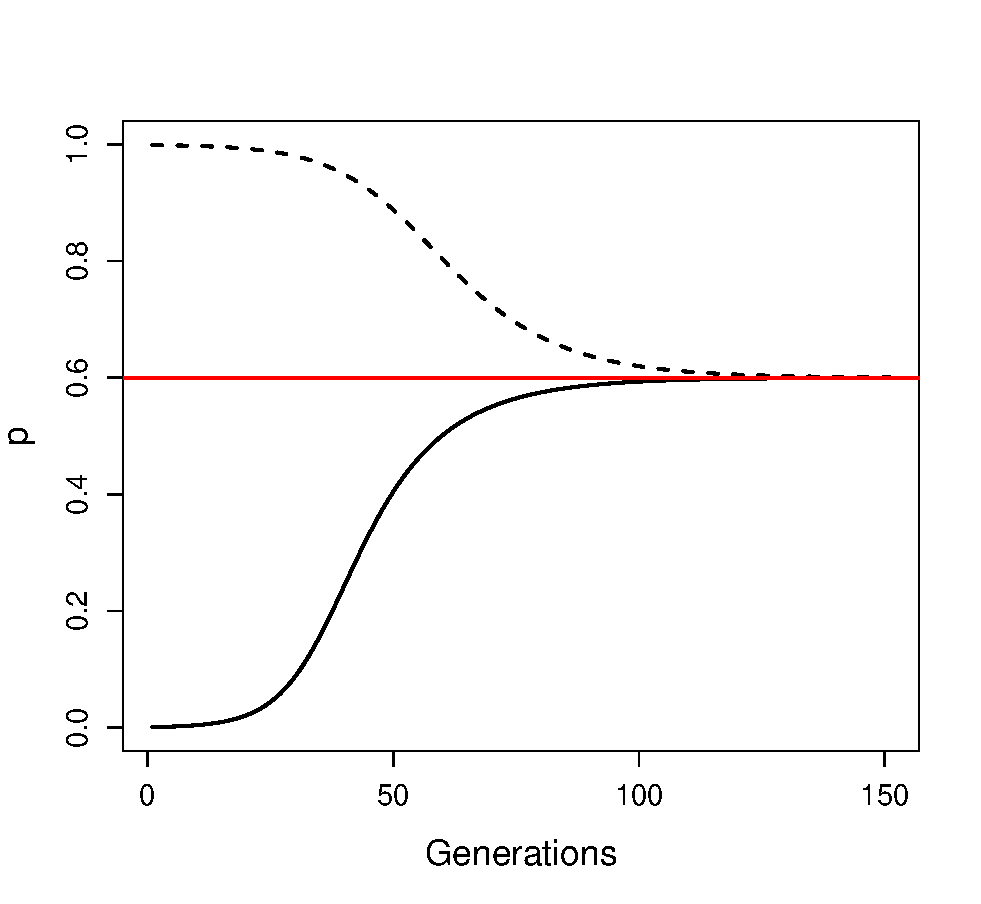
\includegraphics[width = \textwidth]{figures/het_advant_traj.pdf}
\end{center}
\caption{Two allele frequency trajectories of the $A_1$ allele subject to
  heterzygote advantage ($w_{11}=0.9$, $w_{12}=1$, and $w22=0.85$). In
one simulation the allele is started from being rare in the population
($p=\nicefrac{1}{1000}$, solid line) and increases in frequency/ In
the other simulation the allele is almost
fixed ($p=\nicefrac{999}{1000}$, dashed line). In both cases the
frequency moves toward the equilibrium frequency. The red line shows
the equilibrium frequency ($p_e$). \gitcode{https://github.com/cooplab/popgen-notes/blob/master/Rcode/diploid_sel_het_advantage.R}} \label{fig:het_advant_traj}
\end{marginfigure}


In this case, when allele $A_1$ is rare, it is often found in a
heterozygous state, while the $A_2$ allele is usually in the
homozygous state, and so $A_1$ is more fit and increases in frequency. However, when
the allele $A_1$ is common, it is often found in a less fit homozygous state, while
the allele $A_2$ is often found in a heterozygous state; thus it is
now allele $A_2$ that increases in frequency at the expense of allele
$A_1$. Thus, at least in the deterministic model, neither allele can
reach fixation and both alleles will be maintained at an equilibrium frequency as a balanced
polymorphism in the population. 


We can solve for this equilibrium frequency by setting $\Delta p_t = 0$ in  eqn.\ \eqref{deltap_dip2}, 
i.e.\ $p_tq_t (\wbar_1-\wbar_2)=0$. Doing so, we find that there are
three equilibria. Two of them are not very interesting ($p=0$ or
$q=0$), but the third one is a stable polymorphic equilibrium,  where
$\wbar_1-\wbar_2=0$ holds.
Using our $s_1$ and $s_2$ parametrization above, we see that the marginal fitnesses of
the two alleles are equal when
\begin{equation}
	p_e = \frac{s_2}{s_1+s_2} \label{eqn:het_ad_eq}
  \end{equation}
      \begin{marginfigure}
\begin{center}
  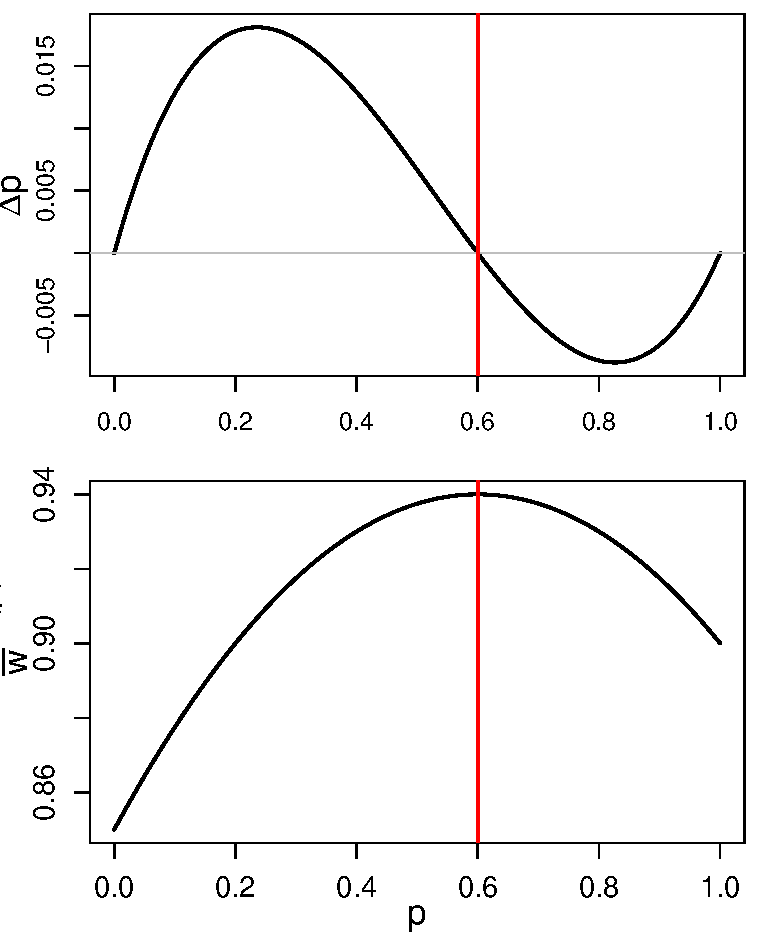
\includegraphics[width = \textwidth]{figures/het_advant_dp_wbar.pdf}
\end{center}
\caption{{\bf Top)} The change in frequency of an allele with heterozygote
  advantage within a generation ($\Delta p$) as a function of the allele
frequency. Fitnesses as in Figure \ref{fig:het_advant_traj}. Note how the frequency change is positive below the
equilibrium frequency ($p_e$) and negative above. {\bf Bottom)} Mean
fitness ($\bar{w}$) as a function of the allele frequency. The red line shows
the equilibrium frequency ($p_e$). \gitcode{https://github.com/cooplab/popgen-notes/blob/master/Rcode/diploid_sel_het_advantage.R}} \label{fig:het_advant_dp_wbar}
\end{marginfigure}
for the equilibrium frequency of interest. This is also the frequency
of $A_1$ at which the mean fitness of the population is maximized. The
highest possible fitness of the population would be achieved if every
individual was a heterozygote. However, Mendelian segregation of alleles in the
gametes of heterozygotes means that a sexual population can never
achieve a completely heterozygote population. This equilibrium
frequency represents an evolutionary compromise between the advantages
of the heterozygote and the comparative costs of the two
homozygotes.\\



\begin{figure}
\begin{center}
  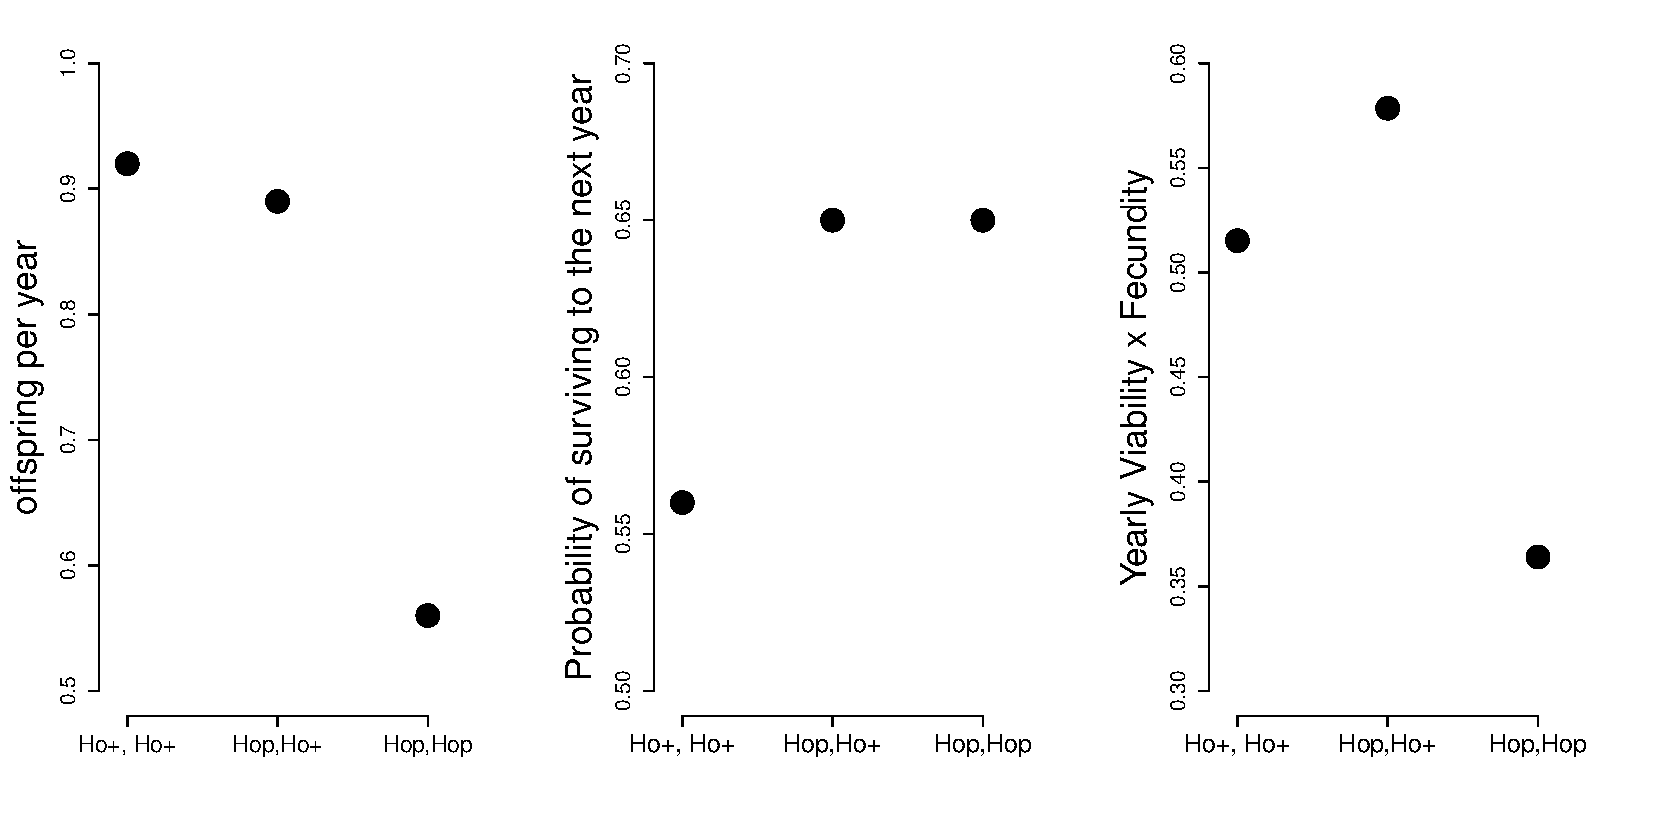
\includegraphics[width = \textwidth]{Rcode/Soay_Sheep/Hopping_sheep_all.pdf}
\end{center}
\caption[][6cm]{For the three Soay sheep genotypes: the offspring per year  ({\bf left}), the probability of
  surviving a year ({\bf middle}), and the product of the two ({\bf
    right}). Thanks to Susan Johnston for supplying these simplified
  numbers from \citet{johnston2013life}. \gitcode{https://github.com/cooplab/popgen-notes/blob/master/Rcode/Soay_Sheep/Soay_Sheep_fitness.R}
} \label{fig:Soay_fitness}
\end{figure}


One example of a polymorphism maintained by heterozygote advantage is
a horn-size polymorphism found in Soay sheep, a population of feral sheep on the island of Soay
(about 40 miles off the coast of Scotland).  The horns of the soay sheep resemble
those of the wild Mouflon sheep, and the male Soay sheep use their horns to defend females during
the rut. \citet{johnston2013life} found a large-effect locus,  at the
RXFP2 gene, that controls much of the genetic variation for horn size. Two
alleles Ho$^p$ and Ho$^+$ segregate at this locus. The Ho$^+$ allele is associated with
growing larger horns, while the Ho$^p$ allele is associated with smaller
horns, with a reasonable proportion of Ho$^p$ homozygotes developing no
horns at all. \citet{johnston2013life} found that the Ho locus had substantial
effects on male, but not female, fitness (see Figure
\ref{fig:Soay_fitness}). \begin{marginfigure}
\begin{center}
  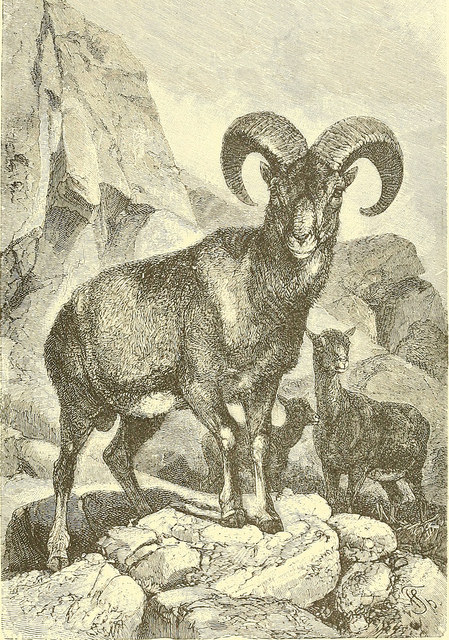
\includegraphics[width = \textwidth]{illustration_images/single_locus_selection/mouflon/18195657882_eb207e4e9e_z.jpg}
\end{center}
\caption{Mouflon ({\it Ovis orientalis orientalis}). \BHLNC{Animate
  creation. (1898). Wood, J. G.}{https://www.flickr.com/photos/internetarchivebookimages/18195657882/in/photolist-oeVkzm-oeVyZM-owqffV-otpyr4-abvEzA-osMSNY-vdEfRm-odZgfB-ot1epP-xvDeKd-yb3aL3-xRUfo4-owdr4T-wJhfme-xj57bn-xAzfXc-xiEcGn-sMnpMH-xP6U3J-w6Wm26-xuMUdr-tHTvam-w6aexB-oubB13-wYKiWR-xnrRBv-xptbR9-wYeGR2-xBHTk1-xvoaiK-xdb5i7-xst4MC-w3QTNe-x9SM4R-xnwGwR-xGd6Qk-xyfL9Q-w3QtPx-wYeJqe}{Smithsonian Libraries} } \label{fig:Mouflon}
\end{marginfigure} The Ho$^p$ allele has a mostly recessive effect on
male fecundity, with the Ho$^p$ homozygotes having lower yearly reproductive
success presumably due to the fact that they perform poorly in male-male
competition (left plot Figure \ref{fig:Soay_fitness}). Conversely, the
Ho$^{+}$ has a mostly recessive effect on viability, with Ho$^{+}$ homozygotes having lower
yearly survival  (middle plot Figure \ref{fig:Soay_fitness}), likely because they spend little time feeding during the rut and so lose substantial body weight. Thus both of the
homozygotes suffer from trade-offs between viability and
fecundity. As a result, the Ho$^p$Ho$^+$ heterozygotes have the highest
fitness  (right plot Figure \ref{fig:Soay_fitness}).  The allele is
thus balanced at intermediate frequency ($~50\%$) in the population due to 
this trade off between fitness at different life history stages.

\marginnote{The fitnesses here are chosen to roughly match those of
  the real Soay sheep example, as a full model would
  require us to more carefully model the life-histories of the sheep. }
\begin{question}
Assume that the frequency of the Ho$^P$ allele is 10\%, that there are 1000 males at birth, and that individual adults mate at random.\\
{\bf A)} What is the expected number of males with each of the three genotypes in the population at birth? \\

{\bf B)} Assume that a typical male individual of each genotypes has the following probability of surviving to adulthood:\\
\begin{tabular}{ccc}
Ho$^+$ Ho$^+$ & Ho$^+$ Ho$^p$ & Ho$^p$ Ho$^p$ \\
0.5 & 0.8 & 0.8
\end{tabular}

Making the assumptions from above,  how many males of each genotype survive to reproduce? 
{\bf C)} Of the males who survive to reproduce, let's say that males with the Ho+Ho+  and Ho+Ho$^p$  genotype have on average 2.5 offspring, while Ho$^p$Ho$^p$ males have on average 1 offspring. Taking into account both survival and reproduction, how many offspring do you expect each of the three genotypes to contribute to the total population in the next generation? \\

{\bf D)} What is the frequency of the Ho+ allele in the sperm that will form this next generation?  \\
{\bf E )} How would your answers to B-D change if the Ho$^p$ allele was at 90\% frequency? \\
\end{question}

\begin{figure}
\begin{center}
  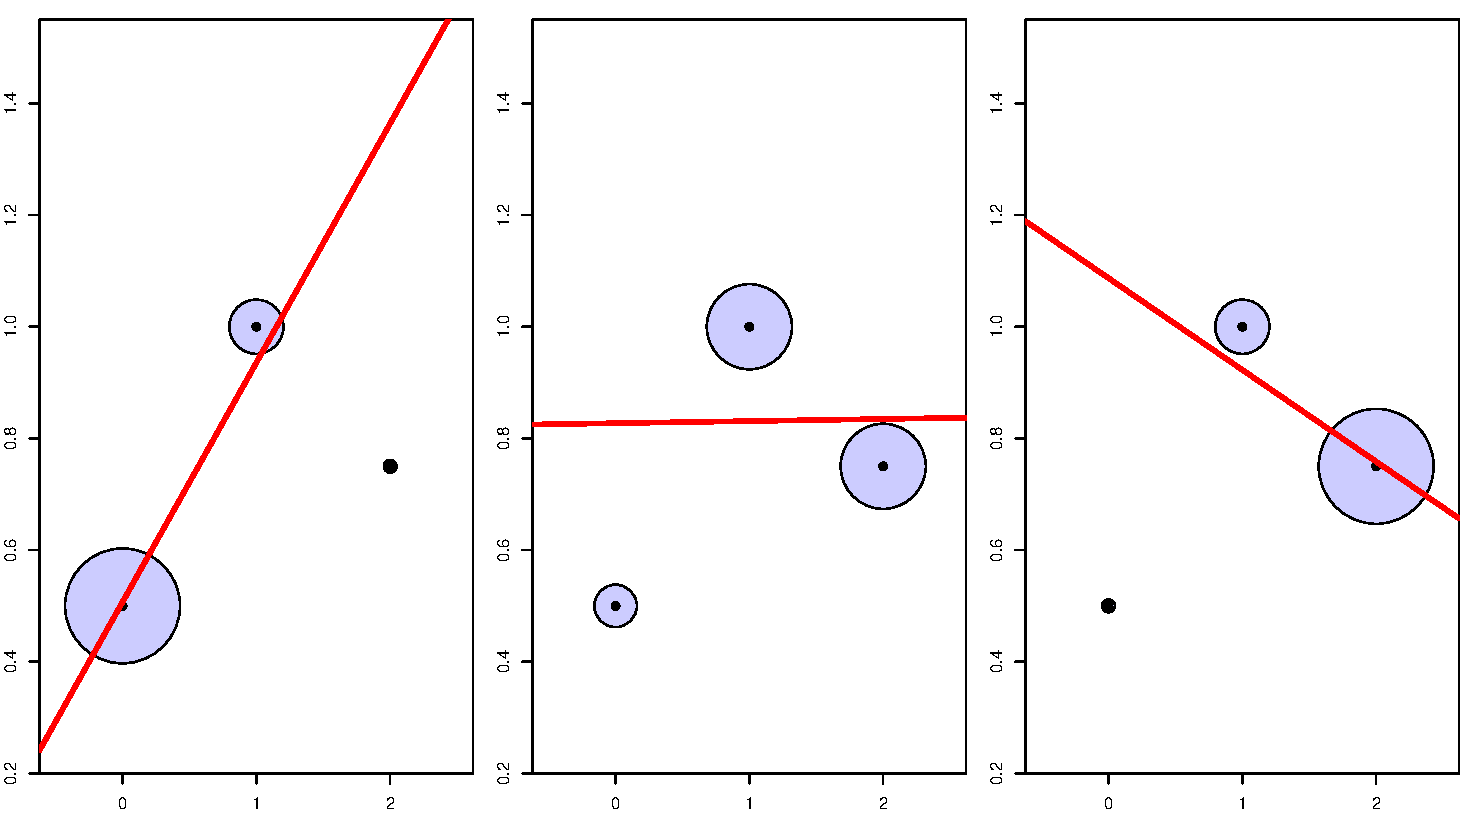
\includegraphics[width = \textwidth]{figures/additive_effect_OverDom.pdf}
\end{center}
\caption{The deviation of the fitness of each genotype away from the mean population
  fitness (0) is shown as black dots. The area of each circle is proportion to the fraction of
the population in each genotypic class ($p^2$, $2pq$, and $q^2$). The
additive genetic fitness of each genotype is shown as
 a red dot. The linear regression between fitness and additive
 genotype is shown as a red line. The black vertical arrows show the
 difference between the average mean-centered phenotype and additive genetic value for each genotype.
The left panel shows $p=0.1$ and the right panel shows $p=0.9$; in the
middle panel the frequency is set to the equilibrium frequency. \gitcode{https://github.com/cooplab/popgen-notes/blob/master/Rcode/Quant_gen/additive_effect.R} } \label{fig:additive_effect_OverDom}
\end{figure}


To push our understanding of heterozygote advantage a little further, note that the marginal fitnesses of our alleles are equivalent to the additive effects of our alleles on fitness. Recall from our discussion of non-additive variation (Section \ref{section:nonAddVar}) that the difference in the additive effects of the two alleles gives the slope of the regression of additive genotypes on fitness, and that there is additive variance in fitness
when this slope is non-zero.  
So what's happening here in our heterozygote advantage model is that the marginal fitness of the $A_1$ allele, the additive effect of allele $A_1$ on fitness, is greater than the marginal fitness of the $A_2$ allele ($\bar{w}_1 > \bar{w}_2 $) when $A_1$ is at low frequency in the population. In this case, the regression of fitness on the number of $A_1$ alleles in a genotype has a positive slope. This is true when the
frequency of the $A_1$ allele is below the equilibrium frequency. If the frequency of $A_1$ is above the equilibrium frequency, then
the marginal fitness of allele $A_2$ is higher than the marginal fitness of allele $A_1$ ($\bar{w}_1 < \bar{w}_2 $) and the regression of fitness on the number of copies of allele $A_1$ that individuals carry is negative. In both cases there is additive genetic variance for fitness ($V_A > 0$) and the population has a directional response. Only when the population is at its equilibrium frequency, i.e. when $\bar{w}_1 =
\bar{w}_2$, is there no additive genetic variance  ($V_A = 0$), as the linear regression of fitness on genotype is zero. 



%%add Drosophila underdom. selection experiement http://courses.biology.utah.edu/seger/3410_spr_09/feb_4_2pp.pdf
\paragraph{Underdominance.} Another case that is of potential interest is the case of fitness
underdominance, where the heterozygote is less fit than either of the two
homozygotes. Underdominance can be parametrized as follows: \\
\begin{center}
\begin{tabular}{lccc}
	genotype & $A_1A_1$ & $A_1A_2$ & $A_2A_2$ \\
	absolute fitness & $w_{11}$ & $>w_{12}<$ & $w_{22}$ \\
	relative fitness (generic) & $w_{11}=W_{11}/W_{12}$ & $w_{12} = W_{12}/W_{12}$ & $w_{22} = W_{22}/W_{12}$ \\
	relative fitness (specific)  & $1+s_1$ & $1$ & $1+s_2$ \\
\end{tabular}\\
\end{center}
\begin{marginfigure}[1.5cm]
\begin{center}
  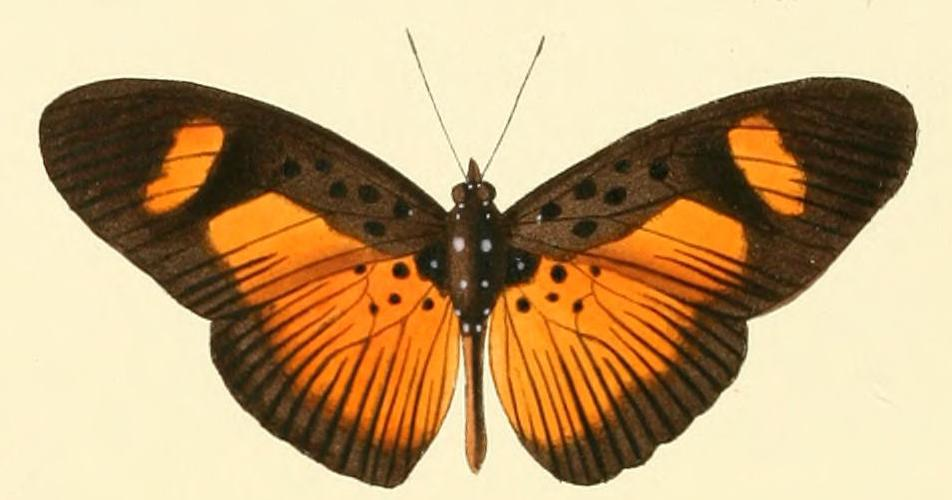
\includegraphics[width = \textwidth]{illustration_images/single_locus_selection/Pseudacraea_eurytus/Pseudacraea_eurytus.JPG}
\end{center}
\caption{In {\it Pseudacraea eurytus} there are two homozygotes morphs that mimic
 a different blue and orange butterfly; the heterozygote fails to mimic
either successfully and so suffers a high rate of predation
\citep{owen1972polymorphic}. \BHLNC{Illustrations of new species of
exotic butterflies (1868) Hewitson.}{https://commons.wikimedia.org/wiki/File:Pseudacraea_eurytus.JPG}{Smithsonian Libraries}} \label{fig:underdom_buttfly}  % https://books.google.com/books?id=4XSmCwAAQBAJ&pg=PA399&lpg=PA399&dq=pseudacraea+eurytus+heterozygotes&source=bl&ots=Dw6f7Wl6rO&sig=oT6VYvO80LEh9dbYKgri-X9OHHQ&hl=en&sa=X&ved=2ahUKEwinoYnWxtXeAhVnw1QKHRj6CzMQ6AEwDXoECAUQAQ#v=onepage&q=pseudacraea%20eurytus%20heterozygotes&f=false
\end{marginfigure}


Underdominance also permits three equilibria: $p=0$, $p=1$, and a
polymorphic equilibrium $p=p_U$. However, now only the first two equilibria are stable, while the polymorphic
equilibrium is unstable. If $p<p_U$, then $\Delta p_t $ is negative
and allele $A_1$ will be lost, while if $p>p_U$, allele
$A_1$ will become fixed.\\


While strongly-selected, underdominant alleles might not spread within populations (if $p_U \gg
0$), they are of special interest in the study of speciation and hybrid zones. That is because alleles $A_1$
and $A_2$ may have arisen in a stepwise fashion, i.e.\ not by a single
mutation,  but in separate subpopulations. In this case, heterozygote disadvantage will play a potential role in species maintenance.\\

      \begin{figure*}
\begin{center}
  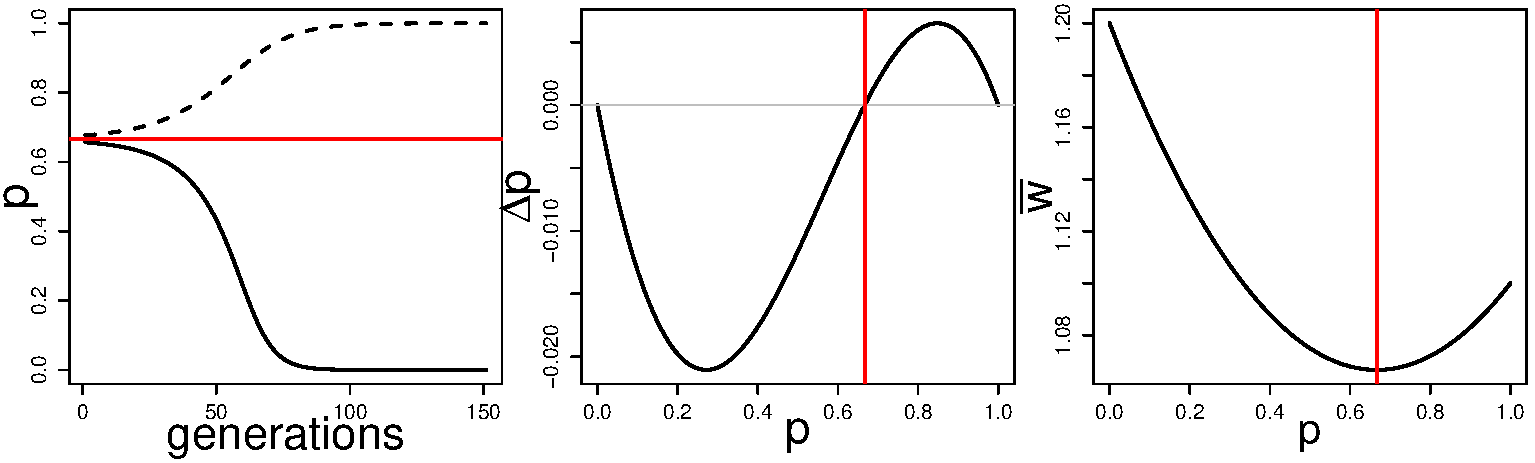
\includegraphics[width = 0.8 \textwidth]{figures/het_disadvant_dp_wbar.pdf}
\end{center}
\caption{
{\bf Left)} Two allele frequency trajectories of an $A_1$ allele subject to
  heterzygote disadvantage ($w_{11}=1.1$, $w_{12}=1$, and
  $w22=1.2$). The allele is started from just above and below the
  equilibrium frequency, in both cases the frequency move away the equilibrium frequency. The red line shows
the unstable equilibrium frequency ($p_e$). 
  {\bf Middle)} The change in frequency of an allele with heterozygote
  disadvantage within a generation ($\Delta p$) as a function of the allele
frequency. Fitnesses as in Figure \ref{fig:het_advant_traj}. Note how the frequency change is negative below the
equilibrium frequency ($p_e$) and positive above. {\bf Right)} Mean
fitness ($\bar{w}$) as a function of the allele frequency. \gitcode{https://github.com/cooplab/popgen-notes/blob/master/Rcode/diploid_sel_het_advantage.R}} \label{fig:het_disadvant_dp_wbar}
\end{figure*}

\begin{question}
You are studying the polymorphism that affects flight speed in butterflies. The polymorphism does not appear to affect fecundity.  Homozygotes for the B allele are slow in flight and so only 40\% of them survive to have offspring. Heterozygotes for the polymorphism (Bb) fly quickly and have a 70\% probability of surviving to reproduce. The homozygotes for the alternative allele (bb) fly very quickly indeed, but often die of exhaustion, with only 10\% of them making it to reproduction.  \\
{\bf A)} What is the equilibrium frequency of the B allele?\\
{\bf B)} Calculate the marginal absolute fitnesses of the B and the b allele at the equilibrium frequency. 
\end{question}


\paragraph{Diploid fluctuating fitness}

Selection pressures fluctuate over time and can potentially maintain
polymorphisms in the population. Two examples of polymorphisms
fluctuating in frequency in response to temporally-varying selection are shown in Figure \ref{fig:Droso_fluct}; thanks to the short
lifespan of {\it Drosophila} we can see seasonally-varying
selection. The first example is an inversion allele in {\it Drosophila pseudoobscura} populations. Throughout western North America, two orientations of the
chromosome, two 'inversion alleles', exist: the Chiricahua and Standard
alleles. \citet{dobzhansky1943} and \citet{wright:46}
investigated the frequency of these inversion alleles over
four years at a number of locations and found that their frequency
fluctuated systematically over the seasons in response to
selection (left side of \ref{fig:Droso_fluct}). If you're still
reading these notes send Prof. Coop a picture of Dobzhansky;
Dobzhansky was one of the most important evolutionary geneticists of
the past century and spent a bunch of time at UC Davis in his later years. Our second example is an insertion-deletion polymorphism in
the Insulin-like Receptor gene in {\it Drosophila melanogaster}. \citet{paaby:14} tracked the
frequency of this allele over time and found it oscillated with the
seasons (right side of \ref{fig:Droso_fluct}). She and her coauthors
also determined that these alleles had large effects on traits such as
developmental time and fecundity, which could mediate the maintenance of this polymorphism through life-history trade-offs.

\begin{figure}
\begin{center}
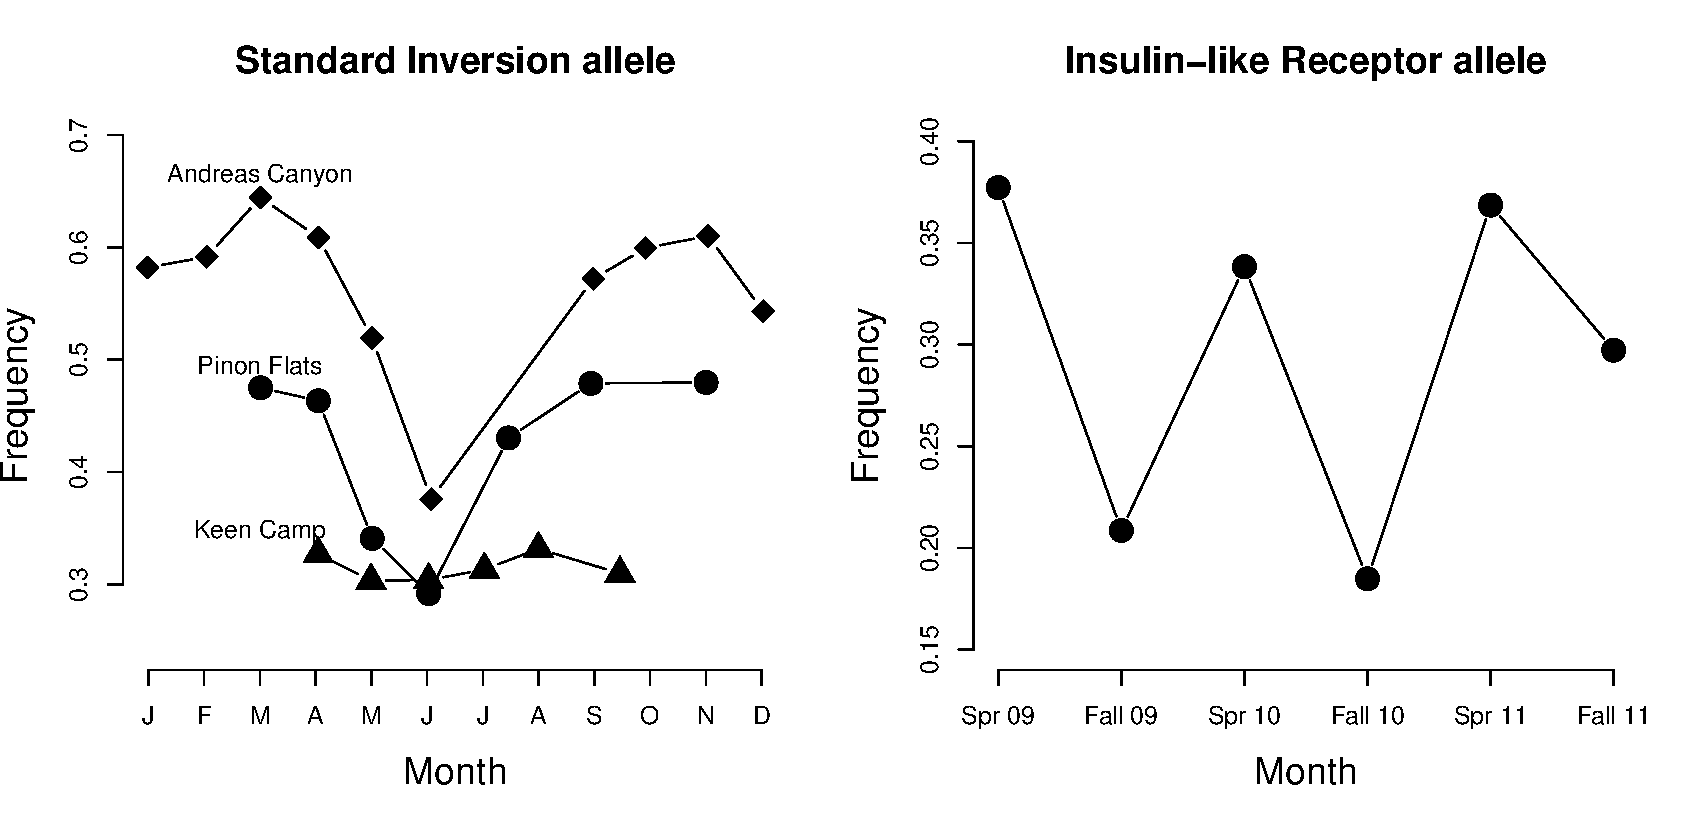
\includegraphics[width=\textwidth]{Journal_figs/single_locus_selection/temporal_Droso_freq/temporal_Droso_freq.pdf}
\end{center}
\caption{{\bf Left)} Seasonal variation in the frequency of the `Standard' inversion allele in
  {\it Drosophila pseudoobscura} for three populations from Mount San
  Jacinto, CA. These frequencies are an average
  over four years. Data from \citet{wright:46}. {\bf Right)} The
  frequency of an allele at the Insulin-like Receptor gene over three
  years in {\it Drosophila melanogaster} samples from an Orchard in
  Pennsylvania. Data from \citet{paaby:14}. \gitcode{https://github.com/cooplab/popgen-notes/tree/master/Journal_figs/single_locus_selection/temporal_Droso_freq}} \label{fig:Droso_fluct} 
\end{figure}

To explore temporal fluctuations in fitness, we'll need to
think about the diploid absolute fitnesses being time-dependent, where the three genotypes  have fitnesses
$w_{11,t}$, $w_{12,t}$, and $w_{22,t}$ in generation $t$. Modeling
the diploid case with time-dependent fitness is much less tractable than the haploid case, as segregation
makes it tricky to keep track of the genotype frequencies.  
However, we can make some progress and gain some intuition by thinking about
how the frequency of allele $A_1$ changes when it is rare
\citep[following the work of ][]{haldane1963}.\\


% (This argument is originally due to Haldane and J. )\\

When $A_1$ is rare, i.e.\ $p_t \ll 1$, the frequency of $A_1$ in the next
generation \eqref{pgen_dip} can be approximated as
\begin{equation}
p_{t+1} \approx \frac{w_{12}}{\wbar} p_t.
\end{equation}
To obtain this equation, we have ignored the $p_{t}^2$ term (because it is very small when $p_t$ is small) and we have assumed that $q_t \approx 1$ in the numerator.
Following a similar argument to approximate $q_{t+1}$, we can write
\begin{equation}
	\frac{p_{t+1}}{q_{t+1}} = \frac{w_{12,t}}{w_{22,t}}  \frac{p_{t}}{q_{t}}.
\end{equation}
Starting from out from $p_0$ and $q_0$ in generation $0$, then $t+1$generations later we have
\begin{equation}
	\frac{p_{t+1}}{q_{t+1}} = \left( \prod_{i=0}^{t} \frac{w_{12,i}}{w_{22,i}}  \right) \frac{p_{0}}{q_{0}}.
\end{equation}
%\erin{I think that this should just be t generations; or if it's t+1
 % generations later on top of the product shouldn't it be t not t-1?
 % Same inconsistency affects the next 2 equations below}
From this we can see, following our haploid argument from above, that the frequency of allele $A_1$ will increase when rare only if
\begin{equation}
	\frac{\sqrt[t]{\prod_{i=0}^{t}w_{12,i}}}{\sqrt[t]{\prod_{i=0}^{t}w_{22,i}}}>1 \label{geometric_1wins},
\end{equation}
i.e. if the heterozygote has higher geometric mean fitness than the $A_2A_2$ homozygote.\\

The question now is whether allele $A_1$ will approach fixation in the population, or whether there are cases in which we can obtain a balanced polymorphism. To investigate that, we can simply repeat our analysis for $q \ll 1$, and see that in that case
\begin{equation}
	\frac{p_{t+1}}{q_{t+1}} = \left( \prod_{i=0}^{t} \frac{w_{11,i}}{w_{12,i}}  \right) \frac{p_{0}}{q_{0}}.
\end{equation}
Now, for allele $A_1$to carry on increasing in frequency and to approach fixation, the $A_1A_1$ genotype has to be out-competing the heterozygotes. For allele $A_1$ to approach fixation, we need the geometric mean of $w_{11,i}$ to be greater than the geometric mean fitness of heterozygotes ($w_{12,i}$).
If instead heterozygotes have higher geometric mean fitness than the $A_1A_1$ homozygotes, then the $A_2$ allele will increase in frequency when it is rare. 
%Therefore, a balanced polymorphism can result when the heterozygote has higher geometric fitness than either of the homozygotes.\\

%\begin{equation}
%\frac{\sqrt[t]{\prod_{i=0}^{t}w_{11,i}}}{\sqrt[t]{\prod_{i=0}^{t}w_{22,i}}}>1
%\end{equation}
%implying that our $11$ homozygotes have to have higher geometric mean
%fitness than our heterozygotes.
%\begin{equation}
%\frac{\sqrt[t]{\prod_{i=0}^{t}w_{11,i}}}{\sqrt[t]{\prod_{i=0}^{t}w_{22,i}}}<1  \label{geometric_2wins}
%\end{equation}
%(satisfying both \eqref{geometric_1wins} and
%\eqref{geometric_2wins}).

Intriguingly, we can thus have a balanced polymorphism even if the heterozygote is never the fittest genotype in any generation, as long as the heterozygote has a higher geometric mean fitness than either of the homozygotes. In this case, the heterozygote comes out ahead when we think about long-term fitness across heterogeneous environmental conditions, despite never being the fittest genotype in any particular environment. %\erin{replaced the sentence below with a new one above, hoping to reduce some of the repetition while still emphasizing the same concept}%In this case, the polymorphism will remain balanced in the population, despite the fact that the heterozygote is never the fittest genotype.

%To see
%this, consider the simple example, where there are two environments
%alternate from generation to generation:\\
%\begin{tabular}{lccc}
%genotype & $A_1A_1$ & $A_1A_2$ & $A_2A_2$ \\
%relative fitness in environment A & $w_{11,A}$ & $>w_{12,A}>$ & $w_{22,A}$ \\
%relative fitness in environment B  & $w_{11,B}$ & $<w_{12,B}<$ & $w_{22,B}$ \\
%Geometric mean fitness & $w_{11,B}$ & $<w_{12,B}>$ & $w_{22}$ \\
%\end{tabular}\\


As a toy example of this type of balanced polymorphism, consider a plant population found in one of two different environments each
generation. These occur randomly; $\nicefrac{1}{2}$ of time the population
experiences the dry environment and with probability $\nicefrac{1}{2}$ it
experiences the wet environment. The absolute fitnesses of the genotypes in the different environments
are as follows:
\begin{center}
\begin{tabular}{cccc} 
Environment & AA & Aa & aa \\
\hline 
Wet & 6.25 & 5.0 & 3.75 \\
  Dry & 3.85 & 5.0 & 6.15\\
arithmetic mean & 5.05 & 5.0 & 4.95\\
\end{tabular}
\end{center}
%{\bf A)} Show whether the equilibrium frequency of A will be $0$, $1$, or in between.\\
{%\bf B)} If the probabilities of wet and dry environments were equal,
%(i.e. 0.5) how would your conclusion change?\\
%(HINT:
\marginnote{This example is loosely based on the work of
  \citet{schemske2001perspective} on {\it Linanthus parryae}, a desert
  annual, endemic to California. There
  are blue- and a white-flowered colour morphs polymorphic many populations,
with this polymorphism being controlled by a single dominant allele. The blue-flowered plants
  produce more seeds in dry years, i.e. they have higher fitness in
  these years, while the white-flowered plants have higher seed
  production in wet years. Thus both morphs can potentially be
  maintained in the population. See \citet{turelli2001stable} for a more
detailed analysis.}
  
Let's write $w_{AA,\text{dry}}$ and $w_{AA,\text{wet}}$ for the fitnesses of the AA homozygote in the two environments. Then, if the
two environments are equally common, $\prod_{i=0}^{t}w_{AA,i} \approx w_{AA,\text{dry}}^{\nicefrac{t}{2}}
w_{AA,\text{wet}}^{\nicefrac{t}{2}}$ for large values of $t$. To
obtain an estimate of this product normalized over the $t$ generations,
we can take the $t^{th}$ root to obtain the geometric mean fitness. Taking the $t^{th}$ root, we find the geometric mean fitness of the AA allele  is $w_{AA,\text{dry}}^{\nicefrac{1}{2}}
w_{AA,\text{wet}}^{\nicefrac{1}{2}}$. Doing this for each of our
genotypes, we find the geometric mean fitnesses of our alleles to be:
\begin{center}
\begin{tabular}{cccc} 
& AA & Aa & aa \\
\hline 
Geometric mean & 4.91 & 5.0 & 4.80\\
\end{tabular}
\end{center}
i.e. the heterozygote has higher geometric mean fitnesses than either of
the homozygotes, despite not being the fittest genotype in either
environment (nor having the highest arithmetic mean fitness). So the $A_1$ allele can invade the population when it is rare as it spread thanks to the higher fitness of the heterozygotes. Similarly the $A_2$
allele can invade the population when it is rare. Thus both alleles
will persist in the population due to the environmental fluctuations,
and the higher geometric mean fitness of the heterozygotes. 


%\erin{I think your solution calculations below switch wet and dry environments (wet has prob 2/3 occurring)}
%> (6.25)^(1/3)*(3.85)^(2/3);(5)^(1/3)*(5)^(2/3);(3.75)^(1/3)*(6.15)^(2/3)
%[1] 4.524812, 5, 5.215074
% (6.25)^(1/2)*(3.85)^(1/2);(5)^(1/2)*(5)^(1/2);(3.75)^(1/2)*(6.15)^(1/2)
% 4.905354, 5, 4.802343



\paragraph{Negative frequency-dependent selection.}
In the models and examples above, heterozygote advantage maintains multiple alleles in the population because the common allele has a disadvantage compared to the
other rarer allele. In the case of heterozygote advantage, the
relative fitnesses of our three genotypes are not a function of the
other genotypes present in the population. However, there's a broader set of models where the relative fitness of a genotype depends on the
genotypic composition of the population; this broad family of models
is called frequency-dependent selection. Negative frequency-dependent selection, where the fitness of an allele
(or phenotype) decreases as it becomes more common in the population, can act to maintain genetic and phenotypic diversity within populations. While cases of long-term heterozygote advantage may be somewhat rare in nature, negative frequency-dependent selection is likely a common form of
balancing selection.

One common mechanism that may create negative frequency-dependent
selection is the interaction between individuals within or among
species. For example, negative frequency-dependent dynamics can
arise in predator-prey or pathogen-host dynamics, where
alleles conferring common phenotypes are at a disadvantage because 
predators or pathogens learn or evolve to counter the phenotypic effects of
common alleles.

\begin{marginfigure}
\begin{center}
  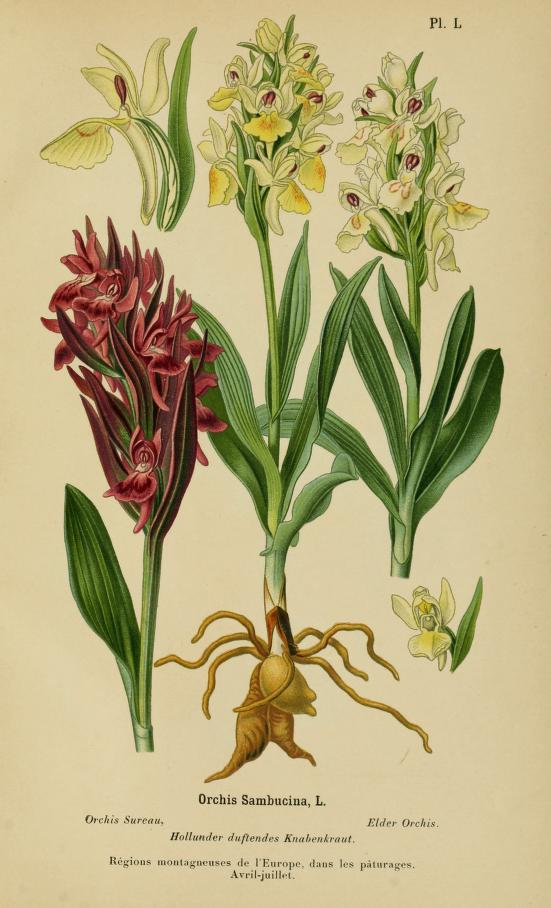
\includegraphics[width = \textwidth]{illustration_images/single_locus_selection/Elderflower_orchid/albumdesorchid1899corr_0209.jpg}
\end{center}
\caption{Elderflower orchid ({\it Dactylorhiza
  sambucina}). \BHLNC{Abbildungen der in Deutschland und den angrenzenden
gebieten vorkommenden grundformen der orchideenarten (1904). Müller, W.}{https://www.biodiversitylibrary.org/page/15349868\#page/126/mode/1up}{New York Botanical Garden} } \label{fig:ElderflowerOrchid}  %Illustrations of the basic forms of orchid species found in Germany and neighboring areas
\end{marginfigure}
As one example of negative frequency-dependent selection, consider the two flower colour morphs in the
deceptive Elderflower orchid ({\it Dactylorhiza
  sambucina}). Throughout Europe, there are populations of these orchids polymorphic for 
yellow- and purple-flowered individuals, with the
yellow flower corresponding to a recessive allele. Neither of
these morphs provide any nectar or pollen reward to their bumblebee
pollinators. 
Thus these plants are typically pollinated by newly emerged
bumblebees who are learning about which plants offer food rewards,
with the bees alternating to try a different coloured flower if they
find no food associated with a particular flower-colour morph \citep{smithson1997negative}. 
\citet{gigord2001negative} explored whether this behaviour by bees
could result in negative frequency-dependent selection; out in the field, the researchers set up
experimental orchid plots in which they varied
the frequency of the two colour morphs. Figure \ref{fig:Elderflower_orchids_fitness} shows their measurements of the relative
male and female reproductive success of the yellow morph across these experimental plots. When the yellow morph is rare, it has
higher reproductive success than the purple morph, as it receives a
disproportionate number of visits from bumblebees that are dissatisfied
with the purple flowers. This situation is reversed when the yellow
morph becomes common in the population; now the purple morph
outperforms the yellow morph. Therefore, both colour morphs are
maintained in this population, and presumably Europe-wide, due to this negative frequency-dependent
selection. %The yellow morph is found at $\sim 69\%$ in the region of
%France where this experiment was conducted, consistent with the frequency at which the two
%morphs are predicted to have equal fitness.
% \graham{check
 % recessive?} %http://courses.biology.utah.edu/seger/3410_spr_09/feb_4_2pp.pdf

\begin{figure}
\begin{center}
  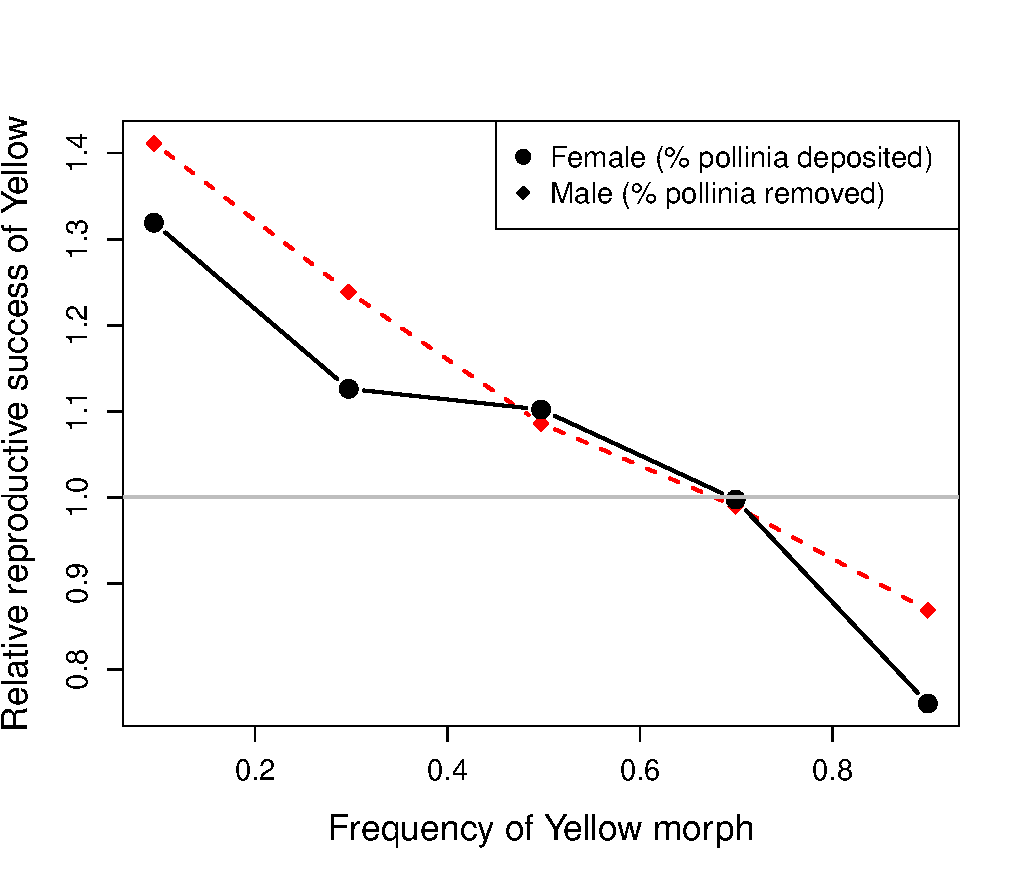
\includegraphics[width = \textwidth]{Journal_figs/single_locus_selection/Elderflower_orchid/Elderflower_orchids_fitness.pdf}
\end{center}
\caption[][0cm]{{\bf Left)} Measures of the relative male- and female- reproductive success of the yellow Elderflower orchid morph
  as a function of the yellow morph in experimental plots. {\bf
    Right)} Two allele frequency trajectories of the Yellow allele
  subject to negative frequency scheme given in the left plot
  (for an initial frequency of $0.01$ and $0.99$, solid and dotted
  line respectively). Note that the yellow 
  Male
  reproductive success is measured in terms of the \% of pollinia
  removed front a plant and female reproductive success is measured in terms of the
  \% of stigmas receiving pollinia on a plant. These measures are made
relative by dividing the reproductive success of the yellow morph by the
mean of the yellow and purple morphs. Pollinia are the pollen masses of
orchids, and other plants, where individual pollinium are transferred
as a single unit by pollinators. Data from
\citet{gigord2001negative}. \gitcode{https://github.com/cooplab/popgen-notes/blob/master/Journal_figs/single_locus_selection/Elderflower_orchid/Elderflower_orchids.R}} \label{fig:Elderflower_orchids_fitness}  
\end{figure}

%The Independents are very aggressive toward each other, but tolerate
%the submissive Satellite males as females are attracted to leks where multiple males display.

Negative frequency-dependent selection can also maintain different 
breeding strategies due to interactions amongst individuals within a population. One
dramatic example of this occurs in ruffs ({\it Philomachus pugnax}), a
marsh-wading sandpiper that summers in Northern Eurasia. The males of this species
lek, with the males gathering on open ground to display and attract females. There are three different male morphs differing in their breeding
strategy. The large majority of males are `Independent', with black or
chestnut ruff plumage, and try to defend and display on small territories. `Satellite' males, with white ruff plumage, make
up $\sim 16\%$ of males and do not defend territories, but rather join
in displays with Independent males and opportunistically mate with
females visiting the lek. Finally, the rare `Faeder' morph was only discovered
in 2006 \citep{jukema2006permanent} and makes up less than 1\% of males. These Faeder males are female mimics who hang
around the territories of Independents and try to 'sneak' in matings with females. Faedar males have plumage closely resembling
that of females and a smaller body size than other males, but with larger testicles (presumably to
take advantage of rare mating opportunities). All three of these
morphs, with their complex behavioural and morpological differences,
are controlled by three alleles at a single autosomal locus, with the
Satellite and Faeder alleles being genetically dominant over the high frequency
Independent allele.
\begin{figure}
\begin{center}   %% pic of a single ruff https://www.biodiversitylibrary.org/page/58888512#page/291/mode/1up
  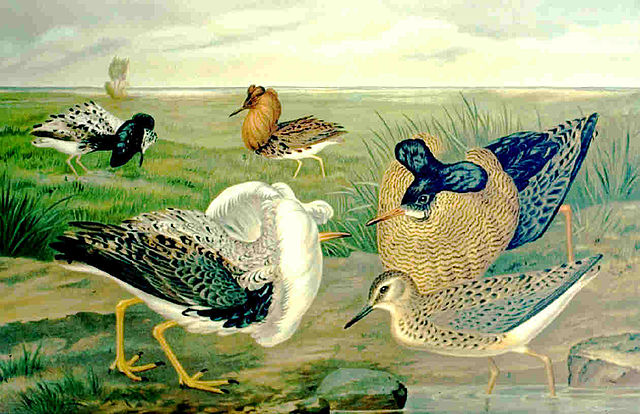
\includegraphics[width = 0.8 \textwidth]{illustration_images/single_locus_selection/Ruffs/Philomachus_pugnax_naumann.jpg}
\end{center}
\caption{Lekking Ruffs ({\it Philomachus pugnax}). Three Independent males, one Satellite male, and one female
(or Faeder male?). {\newline \noindent  \tiny{ Painting by Johann
    Friedrich Naumann (1780–1857). Public Domain,
    \href{https://en.wikipedia.org/wiki/Ruff\#/media/File:Philomachus_pugnax_naumann.jpg}{wikimedia}.}}}\label{fig:Ruff}  
\end{figure}
The genetic variation for these three morphs is potential maintained by
negative frequency-dependent selection, as all three male strategies
are likely at an advantage when they are rare in the population. For
example, while the Satellites mostly lose out on mating opportunities
to Independents, they may have longer life-spans and so may have equal
life-time reproductive success \citep{widemo1998alternative}. However, Satellite and Faeder males
are totally reliant on the lekking Independent males, and so both of
these alternative strategies cannot become overly common in the
population. The locus controlling these differences has been mapped,
and the underlying alleles have persisted for roughly four million years
\citep{kupper2016supergene,lamichhaney2016structural}. While this mating system is
bizarre, the frequency dependent dynamics mean that it has been around
longer than we've been using stone tools. \\ 

While these examples may seem somewhat involved, they must be simple
compared to the complex dynamics that maintain the hundreds of alleles
present at the genes in the Major histocompatibility complex (MHC). MHC
genes are key to the coordination of the vertebrate immune
system in response to pathogens, and are likely caught in an endless arms
race with pathogens adapting to common MHC alleles, allowing rare MHC
alleles to be favoured. Balancing selection at the MHC locus has maintained
some polymorphisms for tens of millions of years, such that some of
your MHC alleles may be genetically more closely related to MHC alleles in other primates than they are to alleles in your
close human friends. 


\section{Sex ratios, sex ratio distorters, and other selfish
  elements. }

We have seen that when selection acts on phenotypes and genotypes in a
frequency-independent manner it can act to
increase the mean fitness of the population, consist with our
notation of selection driving our population to become better adapted
to the environment (eqn. \eqref{eqn:pheno_fitness_landscape} and \eqref{deltap_dip3}). However, when the
absolute fitnesses of individuals are frequency dependent, e.g. depend
on the strategies deployed by others in the population, natural
selection is not guaranteed to increase mean fitness. Nothing about
the strategies pursued by the Ruffs discussed above seems well suited to
maximizing the future growth rate of the population. 
One place where it is particularly apparent that frequency dependence
drives non-optimal solutions from the perspective of the population is in the evolution of a 50/50 sex
ratio. In fact as we'll see, selection can drive the evolution of
traits that are actively harmful to the fitness of an individual when
selection acts below the level of an individual. 

% https://archive.org/stream/aquaticlife51920baus/#page/113/mode/1up
% https://archive.org/stream/aquaticlife51920baus/#page/114/mode/1up 

%Bodmer and A. W. F. EDWARDS sex ratio https://onlinelibrary.wiley.com/doi/pdf/10.1111/j.1469-1809.1960.tb01735.x
%% Edwards on history of sex ratio https://www.jstor.org/stable/pdf/10.1086/286141.pdf?refreqid=excelsior%3A18baef4f72dd7a97685efe161dc66711


\begin{figure}
\begin{center}
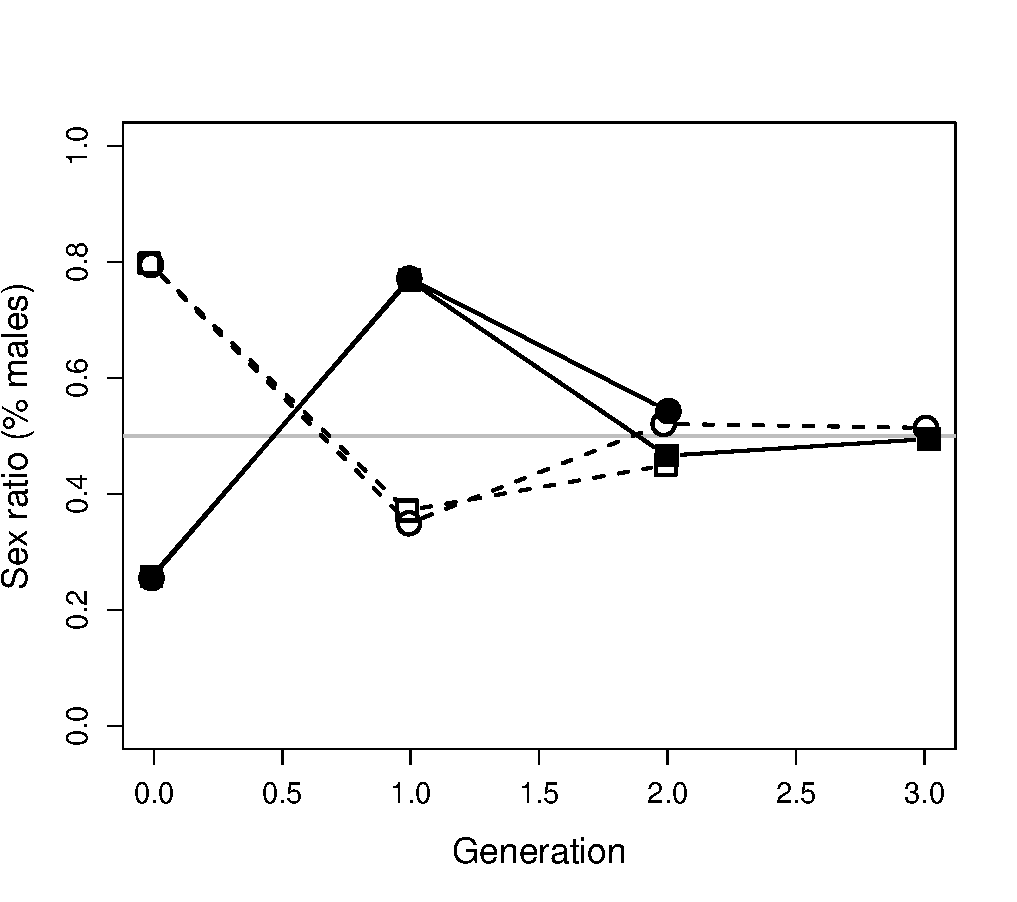
\includegraphics[width= 0.75 \textwidth]{Journal_figs/single_locus_selection/Sex_ratio_basolo/Sex_ratio_basolo.pdf}
\end{center}
\caption{\citet{basolo1994dynamics} explored sex ratio dynamics in platyfish ({\it Xiphophorus
 maculatus}), which has manipulable sex ratio due to its three factor sex determination. She started two replicates with a strong female bias (black) and two replicates with strong male bias (white). In all four cases the sex ratio quickly oscillated to a 50/50 sex ratio.  Data from \citet{basolo1994dynamics}, \gitcode{https://github.com/cooplab/popgen-notes/blob/master/Journal_figs/single_locus_selection/Sex_ratio_basolo/Sex_ratio_basolo.R}} \label{fig:sex_ratio}
\end{figure}

\begin{marginfigure}
\begin{center}
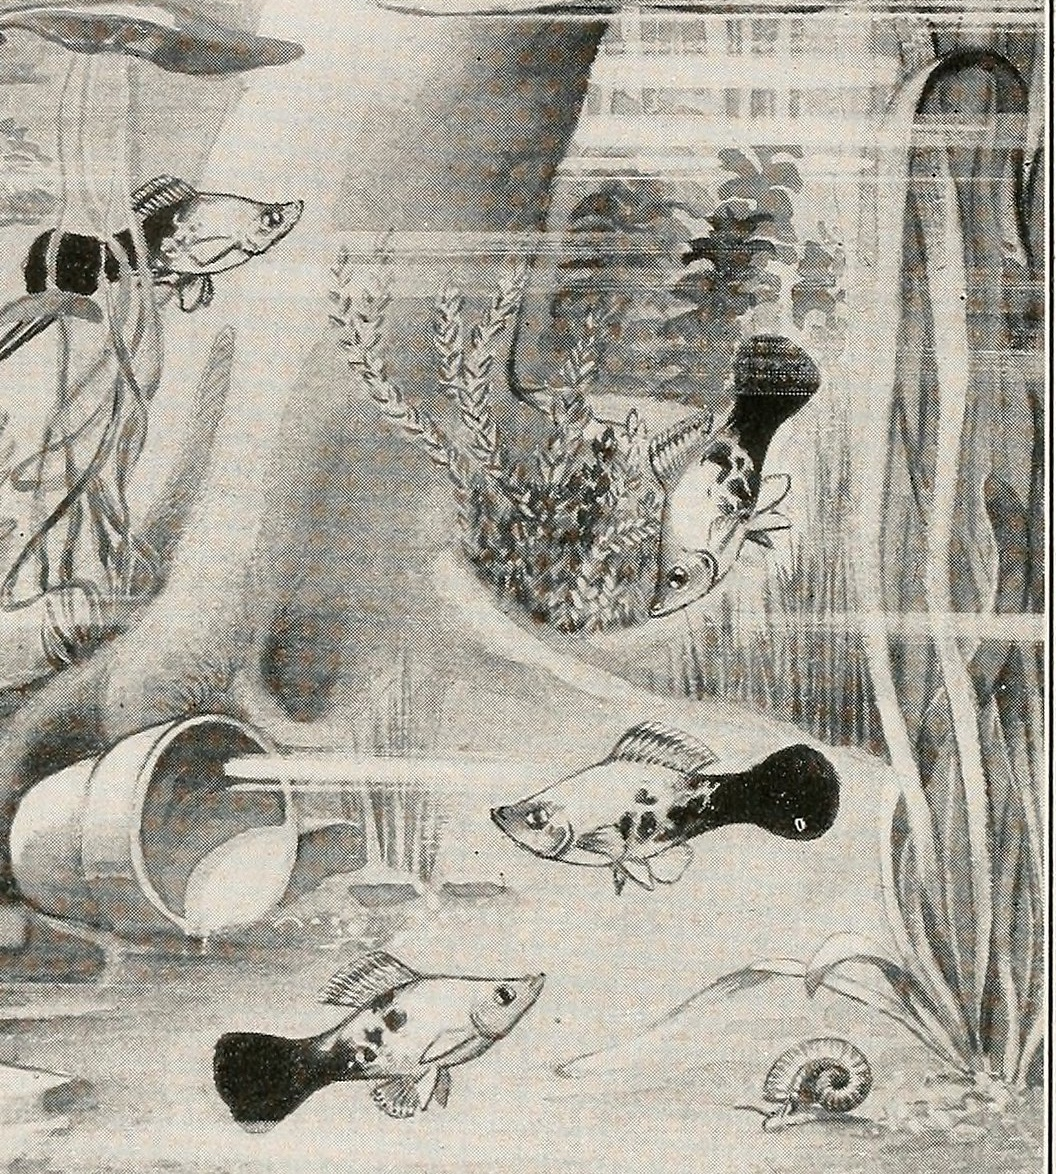
\includegraphics[width= \textwidth]{illustration_images/single_locus_selection/platyfish/Poecilid_Hybrid}
\end{center}
\caption{
  Poecilid Hybrid, {\it Xiphophorus helleri} $\times$ {\it Platypoecilus maculatus}.
%Male and female platyfish ({\it Xiphophorus maculatus}), top and bottom.
\BHLNC{Aquatic life, chapter by Curtis F.S. (1915)}{https://archive.org/stream/aquaticlife51920baus/\#page/113/mode/1up}{Harvard University, Museum of Comparative Zoology, Ernst Mayr Library}} \label{fig:platyfish}
\end{marginfigure}

In many species, regardless of the mechanism of sex determination, the
sex ratio is close to 50/50. Yet this is far from the optimum sex
ratio from the perspective of the population viability. In many
species females are the limiting sex, investing more in gametes and
(sometimes) more in parental care. Thus a population having many
females and few males would offer the fastest rate of population
growth (i.e. the highest mean fitness). Why then is the sex ratio so
often close to 50/50?
Imagine if the population sex ratio was strongly skewed towards females. A rare autosomal allele that caused a mother to produced sons would have high fitness, as the mother's sons would have high reproductive success in this population of most females. Thus our initially rare allele would increase in frequency.
Conversely if the sex ratio was strongly skewed towards males, a rare autosomal allele that causes a mother to produce daughters would spread.
So selection on autosomal alleles favours the production of the rare
sex, a form of negative frequency dependence, and this pushes the sex ratio away from being too skewed. Only the 50/50 sex ratio is evolutionarily stable as there is no rarer sex, and so no (autosomal) sex-ratio-altering mutation can invade a population with a 50/50.
The 50/50 sex ratio is an example of an Evolutionary stable strategy
(ESS), described in more detail in Section
\ref{ESS_sex_Ratio}. \marginnote{``An ESS is a strategy such that, if
  all the members of a population adopt it, then no mutant strategy
  could invade the population under the influence of natural
  selection'' \citet{smith1982evolution}, pg 10.\\ A version of this
  sex ratio argument was first put forward by D{\"u}sing in 1884 and
  popularized by \citet{fisher1930}, see \citet{edwards1998natural}. } %http://www.indiana.edu/~curtweb/L567/readings/JMS%20basic%20game%20theory.pdf
%Our population is held well away from its female-bias optimum for population grow as individual-level selection favours the production of the rarer sex, which results in a 50/50 sex ratio.

%https://commons.wikimedia.org/wiki/File:A_descriptive_catalogue_of_fruit_and_forest_trees,_vines_and_shrubs,_choice_palms_and_roses_(1903)_(20257437763).jpg


\paragraph{Adaptive adjustments to sex ratio in response to local mate
  competition.}

There are, however, situations where we see strong deviations away
from a 50/50 sex ratio. This can represent an adaptive strategy to
situations where individuals compete against relatives for access to resources or
mating opportunities. To see this consider fig wasps. There are many
species of fig wasp, which form a tight pollination symbiosis with many species of 
fig. Wasp females enter the inverted fig flower structure (top right
Figure \ref{fig:fig}) pollinating the flowers. \begin{marginfigure}
  \begin{center}
    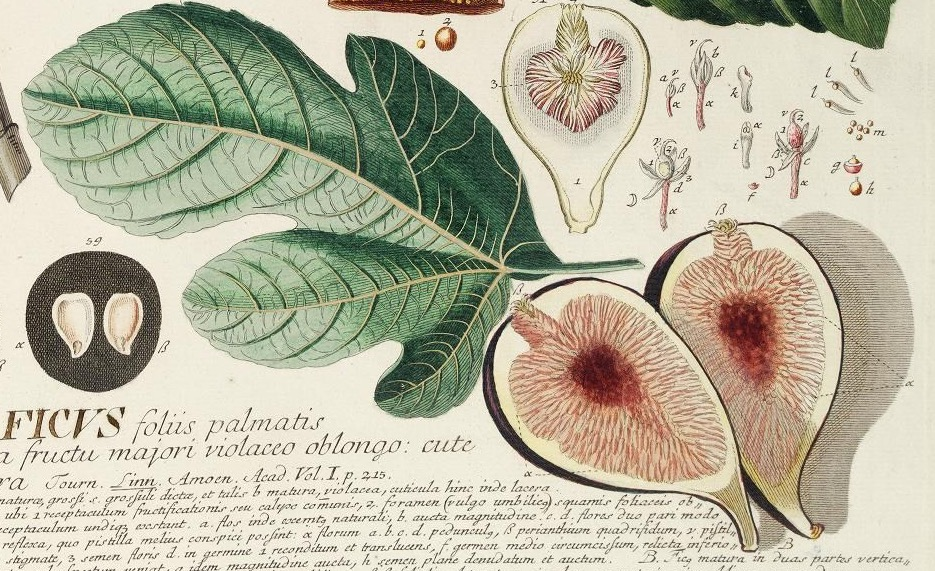
\includegraphics[width=
    \textwidth]{illustration_images/single_locus_selection/Fig_wasp/cropped_fig.png}  %https://www.flickr.com/photos/biodivlibrary/8050635507
\end{center}  % https://commons.wikimedia.org/wiki/File:A_descriptive_catalogue_of_fruit_and_forest_trees,_vines_and_shrubs,_choice_palms_and_roses_(1903)_(20257437763).jpg
\caption{ % alt image https://www.flickr.com/photos/vintage_illustration/41974094471
Common Fig ({\it Ficus carica}). Despite urban legends the crunch in
figs isn't dead wasps, edible figs are dioecious and female wasps
can't lay in the female flowers that form the fruit we eat. 
\BHLNC{Plantae selectae quarum imagines ad exemplaria naturalia Londini, in hortis curiosorum nutrita (1750) Trew, C.J.}{https://www.flickr.com/photos/biodivlibrary/8050635507}{Missouri Botanical Garden}} \label{fig:fig}
\end{marginfigure}
 They lay their eggs in some of the
flowers, which form galls in response.  The young, wingless, male
wasps emerge from their galls first (Figure \ref{fig:fig_wasp}f) but
they never leave the fig. Their only role in this is
to fertilize the female wasps (Figure \ref{fig:fig_wasp}d) in the fig and then die. The female
offspring (Figure \ref{fig:fig_wasp}a \& e) emerge in the fig just as the male fig flowers
are emerging. The female wasps burrow out and and take the fig pollen with them as they fly off.

\begin{marginfigure}
  \begin{center}
    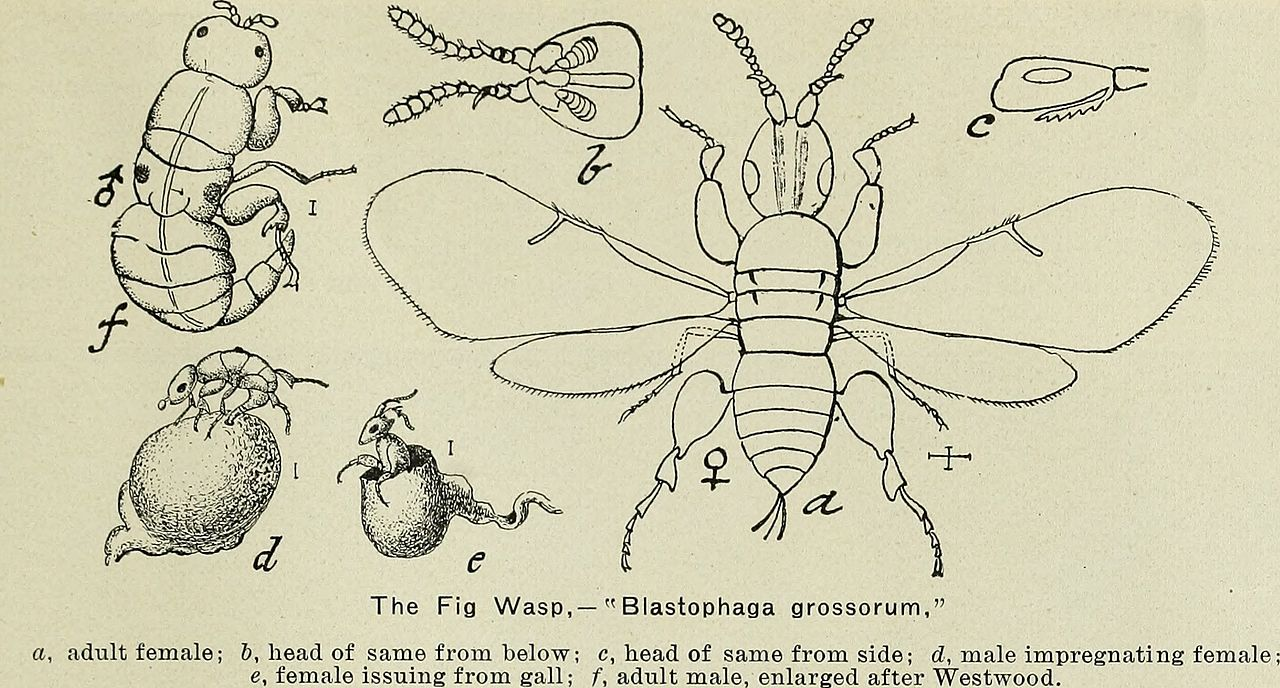
\includegraphics[width= \textwidth]{illustration_images/single_locus_selection/Fig_wasp/1280px-A_descriptive_catalogue_of_fruit_and_forest_trees_vines_and_shrubs_choice_palms_and_roses.jpg}
\end{center}  % https://commons.wikimedia.org/wiki/File:A_descriptive_catalogue_of_fruit_and_forest_trees,_vines_and_shrubs,_choice_palms_and_roses_(1903)_(20257437763).jpg
\caption{
Life stages of Fig wasp ({\it Blastophaga psenes}, synonym {\it Blastophaga
    grossorum}); the primary pollinator of the common fig {\it Ficus carica}.
\BHLNC{A descriptive catalogue of fruit and forest trees, vines and
  shrubs, choice palms and roses (1903) by Fancher Creek
  Nurseries}{https://www.biodiversitylibrary.org/item/164893\#page/33/mode/1up}{National Agricultural Library, USDA}} \label{fig:fig_wasp}
\end{marginfigure}

Female wasps have control over the sex of their offspring but what is their optimal strategy? Females have
this degree of control as sex determination in wasps is haplo-diploid, with fertilized eggs
developing as diploid females and unfertilized as males; by choosing
to lay fertilized eggs they can control their number of daughters. 
If a female wasp lays her eggs into a fig with no other eggs, her sons
will mate with her daughters and then die. Thus a lone female can maximize
her contribution to the next generation by having many daughters, and
just enough sons to fertilize them. And that's exactly what female
wasps do, in many species of fig wasp $95\%$ of individuals born are
female. 
%Figs and fig wasps have an amazing mut

%fig wasps https://science.sciencemag.org/content/228/4701/896
% parasitic wasps https://onlinelibrary.wiley.com/doi/pdf/10.1111/j.1558-5646.1983.tb05520.x

\begin{figure}
\begin{center}
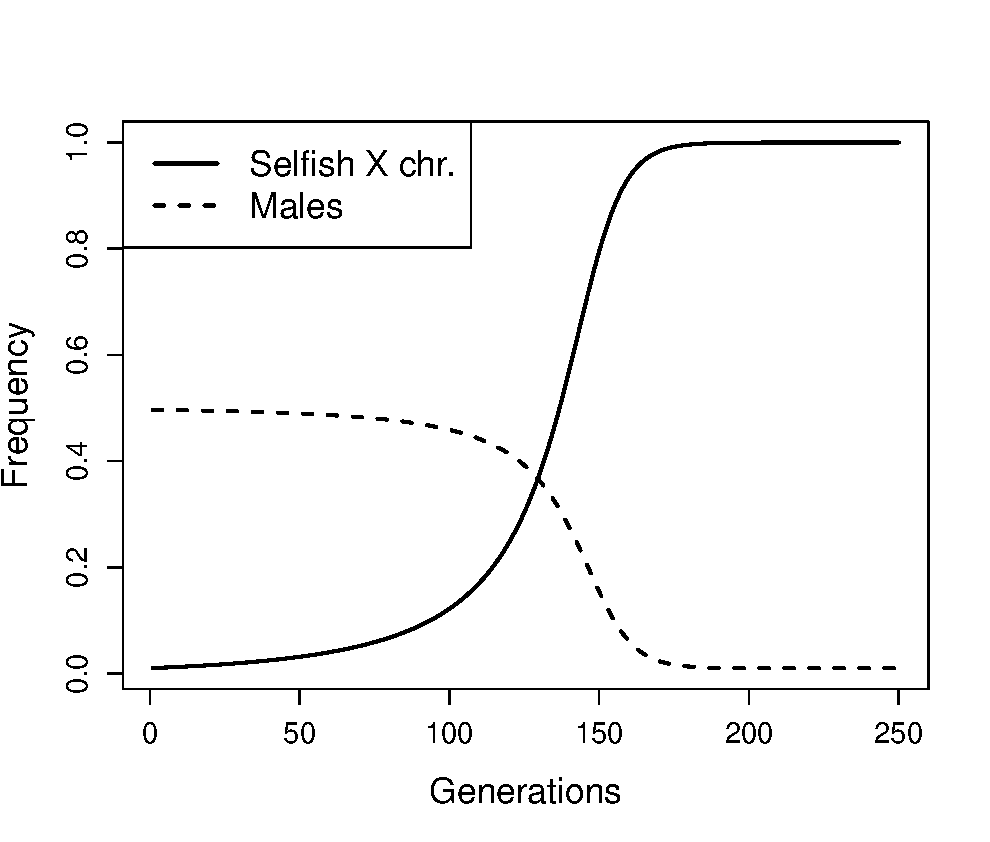
\includegraphics[width= \textwidth]{figures/sex_ratio_distortor.pdf}

\end{center}
\caption[][3cm]{The increase in frequency of a sex-ratio distorting X allele in the population of
  X chromosomes (solid line) and the frequency of males in the
  population. Males carrying the selfish X allele have $99\%$
  daughters, and the selfish X allele reduces the viability of the
  carries by $20\%$ in a dominant manner. The model set up as in \citet{edwards1961population}, \gitcode{https://github.com/cooplab/popgen-notes/blob/master/Rcode/sex_ratio_distortor.R}} \label{fig:selfish_X_freqs}
\end{figure}

\subsection{Selfish genetic elements and selection below the level of
  the individual.}

These ideas about individuals pursuing selfish strategies, which can
lower the populations fitness, extends below the level of the individual. The alleles within an
individual can sometimes pursue selfish strategies that
actively harm the individuals that carry them. Here we'll take a tour
of the rogues gallery of some the various
genetic conflicts that occur and selfish genetic elements that exploit
them. They're included in this chapter in part because much of their biology can
be understood from the perspective of the ideas developed here. But the main reason for talking about them is that they're an
amazing slice of biology. %There's something deeply satisfying about
%the idea that 


\paragraph{Selfish sex chromosomes and sex ratio distortion}
From the perspective of the autosomes a 50/50 sex ratio normally represents
a stable strategy, but all is not always harmonious in the genome. In
systems with XY sex determination, male fertilization by Y-bearing sperm
leads to sons, while male fertilization by X-bearing sperm leads to daughters. 
From the viewpoint of the X chromosome the Y-bearing sperm, and a
male's sons, are an evolutionary deadend. We can imagine a mutation
arising on the X chromosome that causes a poison to be released
during gametogenesis that kills Y-bearing sperm. This would cause much
of the ejaculate of the males carrying this mutation to be X-bearing sperm, and so these males would have mostly
daughters. Such an allele would potentially spread in the population
as it is over transmitted through males, even if it somewhat reduces
the fitness of the individuals who carry it. The spread of this allele would strongly
bias the population sex ratio towards females. Such `selfish' X
alleles turn out to be relatively common, and they can often
substantially low the fitness of the bearer. They do not spread because they are good for the individual but rather because
they are favoured due to selection below the level of the individual.

\begin{marginfigure}[-3cm]
\begin{center}
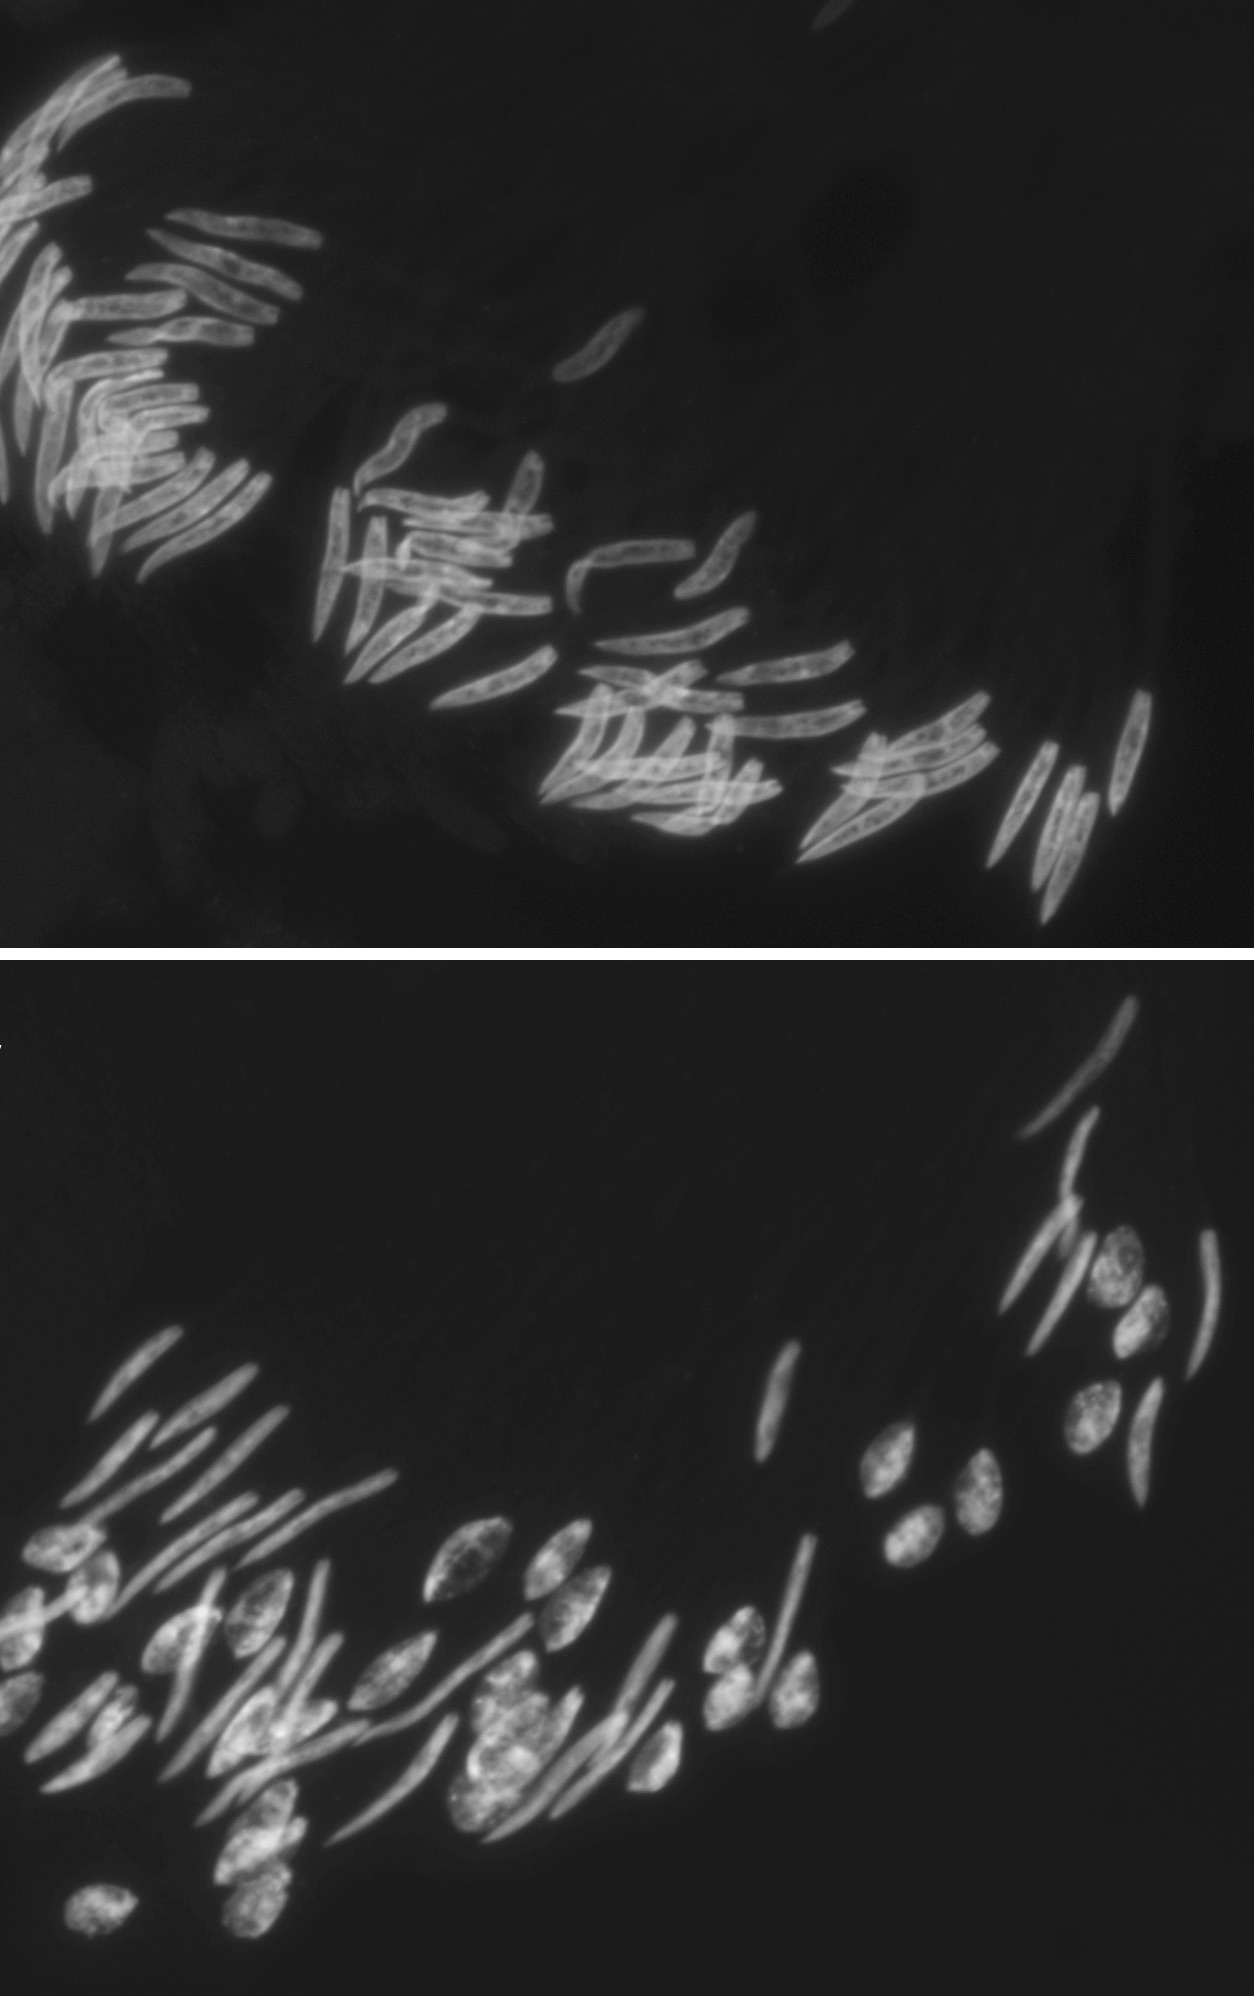
\includegraphics[width= \textwidth]{Journal_figs/single_locus_selection/Winters_sex_ratio_drive/Winters_sex_ratio_drive_sperm.jpg}

\end{center}
\caption{{\bf Top)} Normally developing spermatids in {\it D.
  simulans}. {\bf Bottom)}  Abnormally developing spermatids in a male
expressing {\it dox}. The spermatids that look like
  rice crispies carry the Y chromosome,  the normal, slender
  spermatids are X-bearing spermatids.  Figure from
  \citet{tao2007sex}, cropped, \PLOSccBY. } \label{fig:winters_sperm}
\end{marginfigure}

One example of a selfish X
chromosome allele is the {\it Winters sex-ratio} system found in {\it Drosophila
  simulans}, so named as it was found in flies collected around Winters, California (just a
few miles down the road from Davis). In crosses males carrying the selfish X
chromosome have  $>80\%$ daughters. The gene
responsible, {\it Dox} ({\it Distorter on the X}), is a gene
duplicated by transposition and produces a transcript which targets a region
on the $Y$ chromosome preventing the Y-bearing sperm from developing
\citet[see Figure \ref{fig:winters_sperm} from][]{tao2007sexII}. 

%https://journals.plos.org/plosbiology/article?id=10.1371/journal.pbio.0050292#pbio-0050292-g005
%https://journals.plos.org/plosbiology/article?id=10.1371/journal.pbio.0050303

  \begin{figure}
\begin{center}
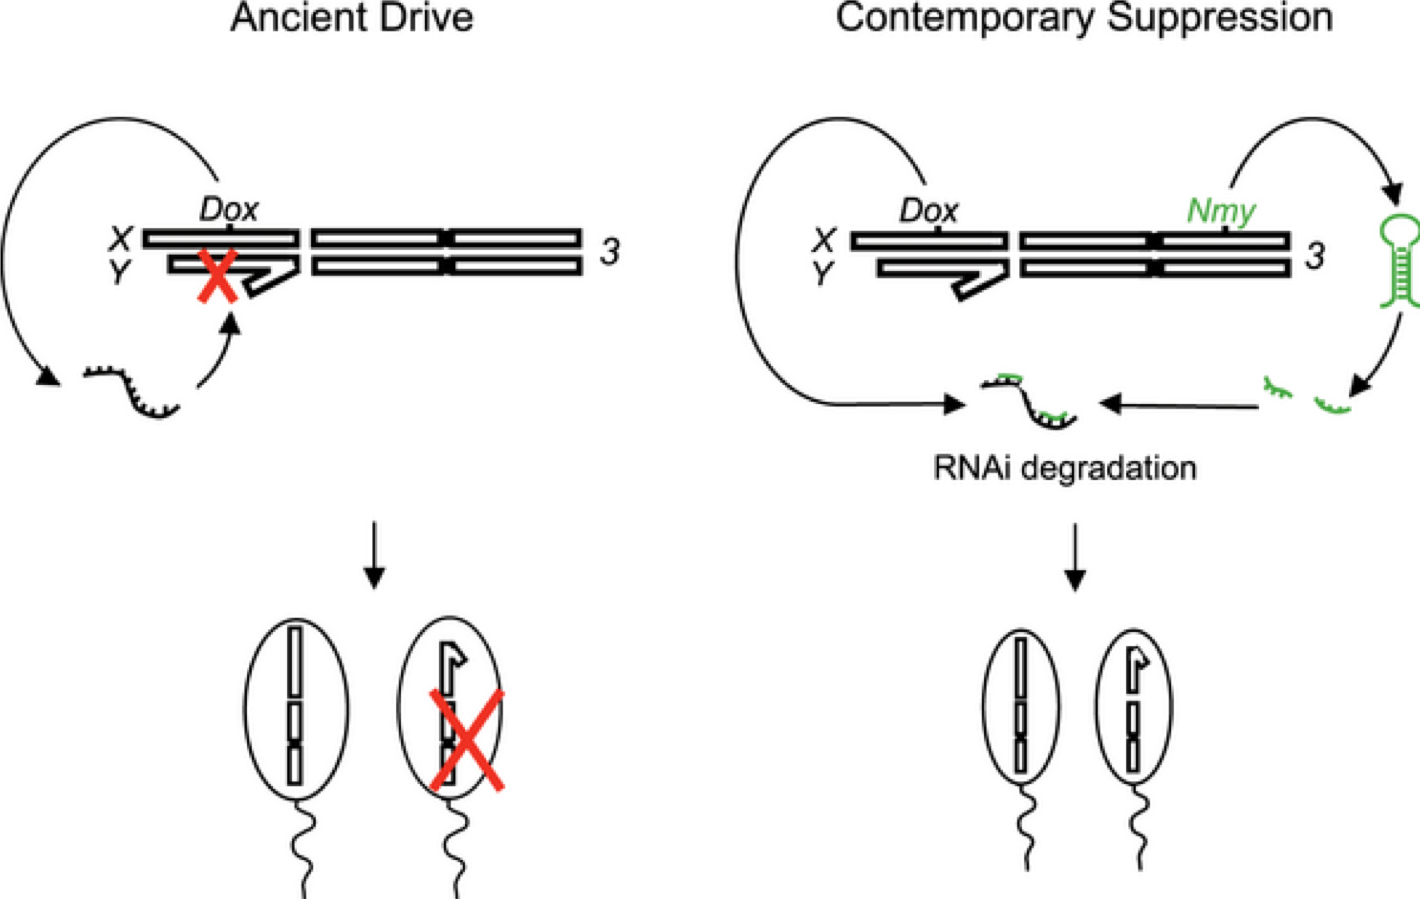
\includegraphics[width= \textwidth]{Journal_figs/single_locus_selection/Winters_sex_ratio_drive/Ferree_Barbash_dox_cartoon.png}
\end{center}
\caption{Mechanistic and Evolutionary Model for sex-ratio Distortion
{\bf Left)} The X-linked Dox gene evolved to target the Y chromosome, blocking
Y-bearing sperm from developing and so favouring its own
transmission. {\bf Right)} Subsequently Dox was retrotransposed to an
autosome forming the Nmy gene. Nmy was subsequently rearranged by a
a small duplication, and now blocks the action of dox by the formation
of a hairpin small interfering RNA. Figure from
\citet{ferree2007distorted}, \PLOSccBY. See \citet
{lin2018hprna} for an update on the fascinating biology and further
loci uncovered in this system.} \label{fig:dox_cartoon}
\end{figure}

The spread of such selfish sex chromosomes, distorting the sex ratio
strongly away from 50/50, can have profound effects for population
growth rates.\sidenote{Indeed people have long discussed using
selfish Y chromosomes, driving an over production of sons, for population control of malaria-spreading
mosquitos. Natural selfish systems on the Y appear rare, likely
because of its low gene content.} However, the other sex chromosome and autosomes are not helpless
against the spread of selfish sex chromosome elements. In the case of
a selfish X chromosome that has achieved appreciable frequency in the population, there will be a strong excess of females
in the population such that suppressors of drive can arise on the autosomes
and spread due to the fact that they  cause the male bearer to
produces some sons and so spread due to Fisherian sex-ratio advantage.
This has happened in the case of the Winters sex chromosome system. An
autosomal allele has spread through the population that suppresses the
selfish X chromosome, restoring the 50/50 sex ratio. Now the sex ratio
distorter can only be found by crosses to naive populations, where the
supressor has not spread yet. The autosomal supressor gene turns out to be
a duplicate of the selfish dox gene,{\it NMY} ({\it Not Much Yang}), that moved to the
autosome through retrotransposition and now blocks the action of dox
through RNA-interference degradation of the dox transcript \citep[
][, see Figure \ref{fig:dox_cartoon}]{tao2007sex}.
%https://journals.plos.org/plosgenetics/article?id=10.1371/journal.pgen.1004822

\graham{Mention Y chromosome fighting back mouse eg?}

\paragraph{Conflict due to maternally transmitted elements.}


%CMS pic https://www.g3journal.org/content/3/10/1727

%%carrot flower https://archive.org/stream/cu31924000606107/#page/n313/mode/1up
% https://science.sciencemag.org/content/106/2763/594

%%sunflower  https://www.flickr.com/photos/biodivlibrary/6059667280/in/photostream/
%% https://en.wikipedia.org/wiki/Lobelia_siphilitica


Chromosomes transmitted maternally, i.e. only through mothers, also have divergent
interests from the individual. Many plants are hermaphrodites producing
both pollen and seeds. But from the perspective of the Mitochondria in
an individual, pollen is a waste of energy as the Mitochondria won't
be transmitted through it. Thus a mutation that arises on the
Mitochondria abolishing male sexual function (pollen) and shunting energy into
other processes can spread. 
The self spread of a Cytoplasmic Male
Sterility (CMS) allele creates a population
of females and hermaphrodite plants (a gynodioecious population).
%\sidenote{this mixed population is called a gynodioecious population},
This strong excess of female plants in
turn can select for the spread of autosomal suppressors of CMS that are
favoured by producing the rarer gamete (pollen), and so restore the
population to hermaphroditism.   \begin{marginfigure}
\begin{center}
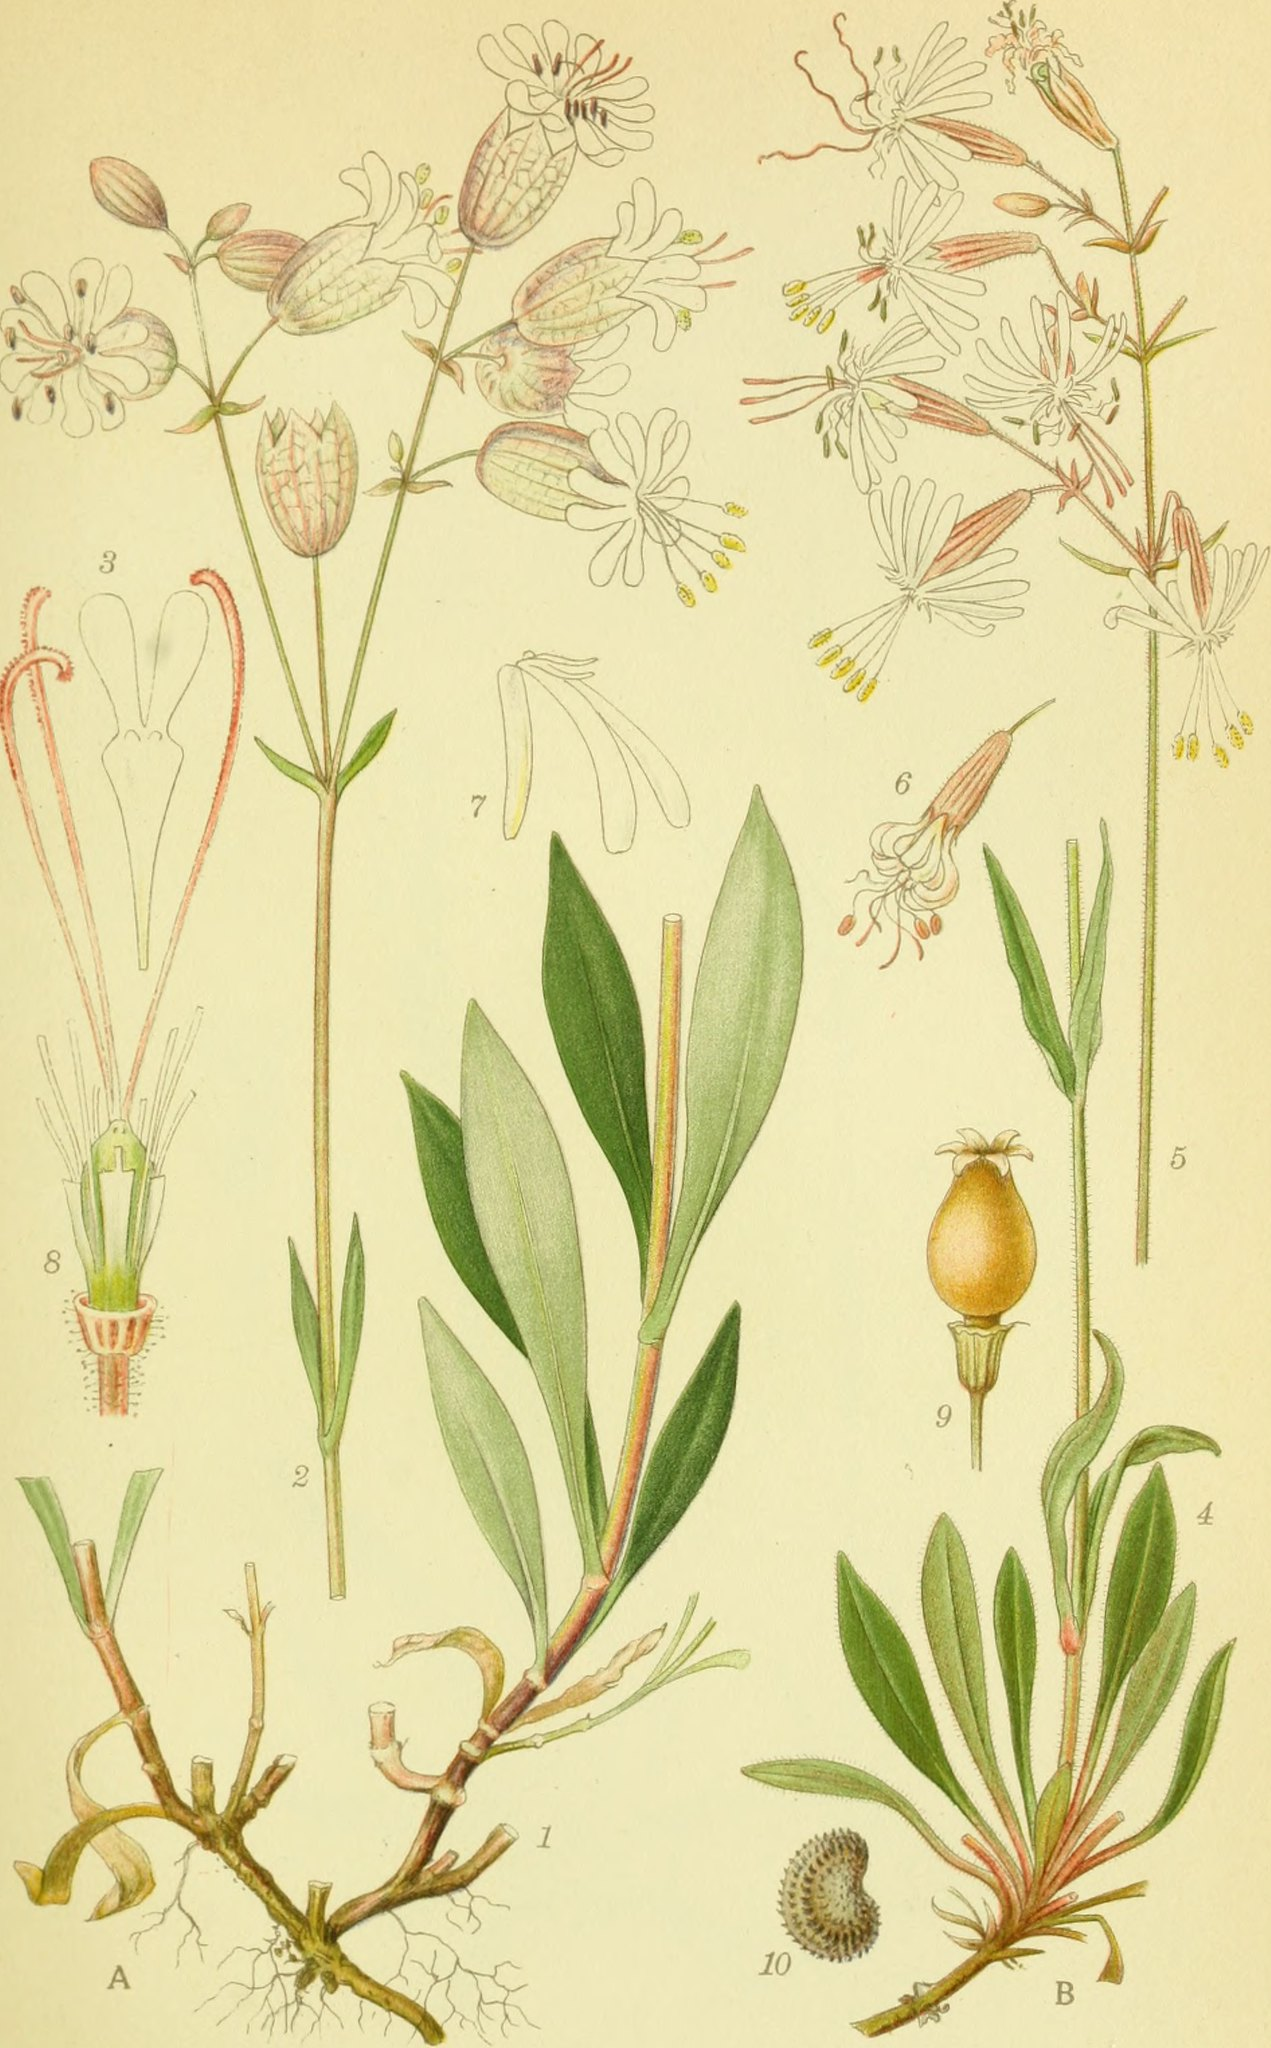
\includegraphics[width= \textwidth]{illustration_images/single_locus_selection/Silene_vulgaris/20184393949_9e22db5ff4_k.jpg}
\end{center}
\caption{Bladder Campion  ({\it Silene vulgaris}), on left, has both 
hermaphrodite and female plants due to CMS and nuclear
restorer polymorphisms \citep{charlesworth1998male}. ({\it
    S. nutans} on right) \BHLNC{Billeder af nordens flora
    (1917). Mentz, A}{https://archive.org/stream/billederafnorden02ment/\#page/n160/mode/1up}{The LuEsther T Mertz Library, the New York Botanical Garden} } \label{fig:Bladder_Campion}
\end{marginfigure}  % https://archive.org/stream/billederafnorden02ment/#page/n160/mode/1up
 The spread of such CMS alleles, and subsequent autosomal suppression, is thought to be common in hermaphrodite
species and often uncovered in crosses between diverged hermaphrodite populations.
The discovery or deliberate creation of CMS alleles in agricultural plants is
prized because it gives breeders more control over hybridization as
they can more carefully control the pollen donor to the plants.

The maternal transmission of mtDNA also causes genetic conflicts in organisms
with separate sexes. Males are an evolutionary dead end as far as
mitochondria are concerned, and so mitochondrial mutations that lower a male's
fitness are not removed from the population of mitochondria. Thus the
Mitochondria genome may be a hotspot of alleles that are deleterious in males
\citep[an effect termed the ``Mother's curse''][]{}.
 \begin{figure}
\begin{center}
  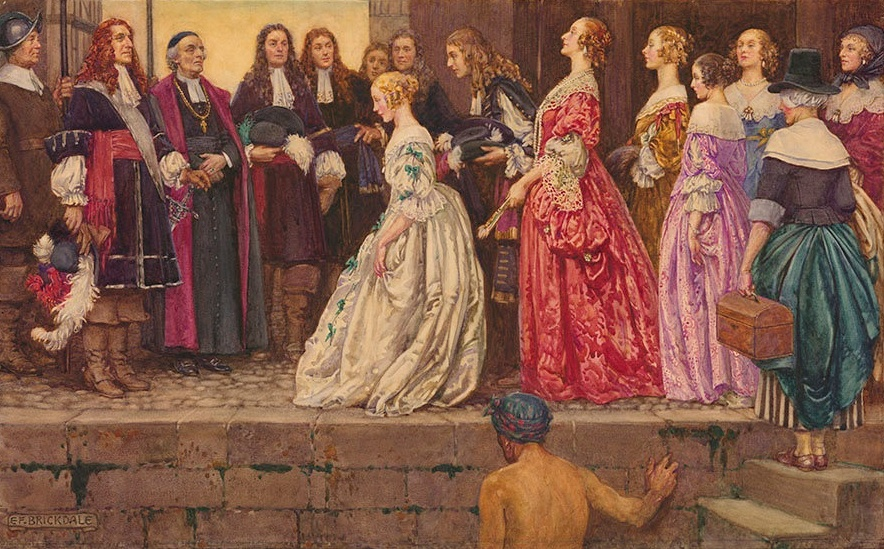
\includegraphics[width= \textwidth]{illustration_images/single_locus_selection/fille_du_roi/fille_du_roi.png}
\end{center}
\caption[][5cm]{Arrival of the fille du roi, the `king's daughters' to
  Quebec city in 1667. Painting
  by Eleanor Fortescue-Brickdale.  The fille du roi were some 800 women whose emigration to New France (Quebec) was paid for by an program established by
  King Louis XIV of France to address the strong gender imbalance of
  the new colony. You can read more in this \href{https://www.theatlantic.com/science/archive/2017/09/how-a-fille-du-roy-brought-the-mothers-curse-to-canada/540153/}{Atlantic article} by Sarah Zhang.
\newline \noindent \tiny{
 Painting from the Library and Archives Canada collection,
 \href{https://commons.wikimedia.org/wiki/File:Arrival_of_the_Brides_-_Eleanor_Fortescue-Brickdale.png}{Wikimedia},
 Public Domain.}} \label{fig:fille_du_roi}  %http://collectionscanada.gc.ca/pam_archives/index.php?fuseaction=genitem.displayItem&lang=fre&rec_nbr=2896937&rec_nbr_list=2896937
\end{figure}
% fille-du-roy
% https://en.wikipedia.org/wiki/King%27s_Daughters#/media/File:Arrival_of_the_Brides_-_Eleanor_Fortescue-Brickdale.png 
One example of a male-deleterious mitochondrial mutations underlying
Leber’s `hereditary optic neuropathy' (LHON) in humans. LHON causes degeneration
of the optic nerve and loss of vision in teenage males (with much
lower penetrance in women). One such LHON mutation is present at low
frequency in the Quebec population. The  Qu{\'e}b{\'e}cois population grew
rapidly from a relatively small number of founders, leading to the
prevalence of some disease mutations due to the founder effect. Thanks to the detailed
genealogical records kept by French Canadians since the founding of
Quebec, we know that nearly all the Qu{\'e}b{\'e}cois LHON alleles are
descended from the mitochondria of a single woman, one of the {\it fille du roi}, who arrived in Quebec City
in 1669 \citep{laberge2005fille}.  Using the genealogy, \citet{milot2017mother} tracked all
of her mitochondrial descendents, individuals whose mothers were in her
matrilineal line, and so identified all the individuals in the
Qu{\'e}b{\'e}cois who carried this allele.
There was no significant difference in the fitness of females who
carried or didn't carry the mutation. In contrast, the fitness of male carriers of the mutation was only 65.3\% that of male non-carriers. 
This mitochondria mutation has increased in frequency slightly over the past 290
years, despite its strong effects in males, due to the fact that its effects have no consequence for female fitness.

\begin{question}
The frequency of the LHON allele was roughly $\nicefrac{1}{2000}$ in
1669. If females suffered the same ill consequences as males what
would be the frequency today? [assume there are $\sim$29 years a generation]
\end{question}

\begin{question}
Kin selection has been proposed as a way that the male deleterious
mitochondrial mutations could be removed from the
population. Can you explain this idea?
\end{question}  

  \begin{marginfigure}
\begin{center}
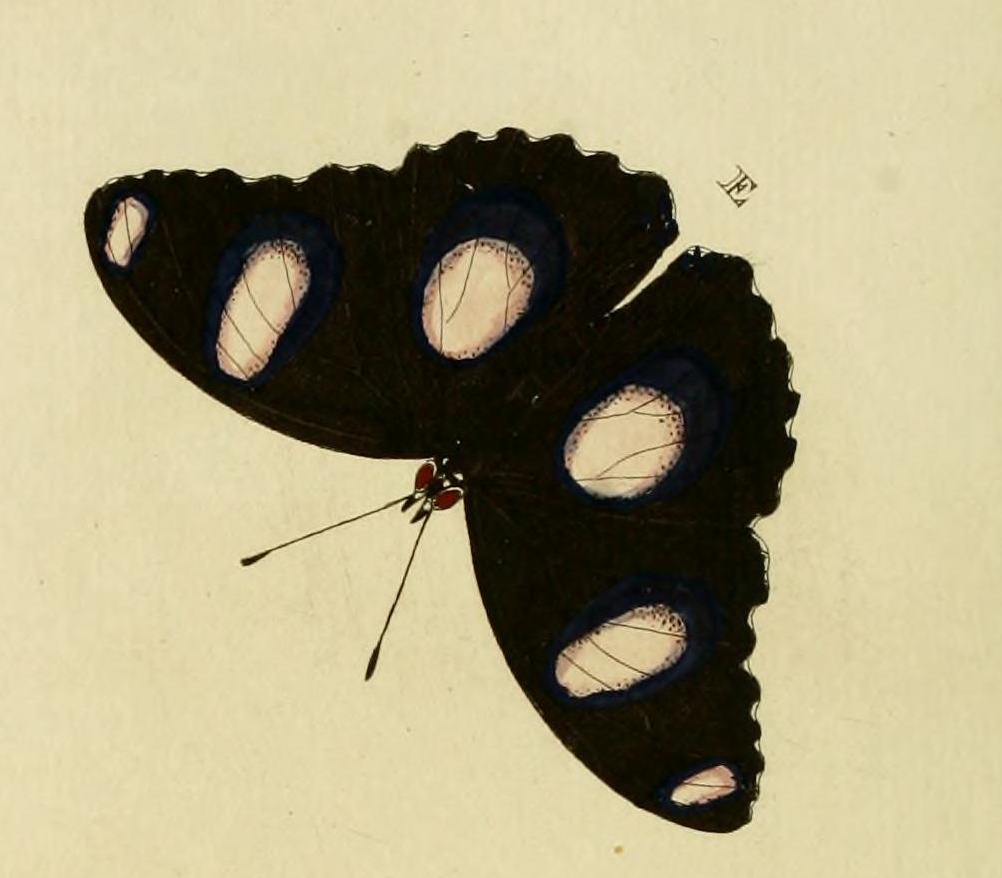
\includegraphics[width= \textwidth]{illustration_images/single_locus_selection/Hypolimnas_bolina/Hypolimnas_bolina.png}
\end{center}
\caption{male Eggspot butterfly ({\it Hypolimnas bolina}). \BHLNC{P. Cramer's Uitlandsche kapellen (1780)}{https://www.biodiversitylibrary.org/title/43777\#page/292/mode/1up}{Smithsonian Libraries} } \label{fig:Hypolimnas_bolina}
\end{marginfigure}  % https://commons.wikimedia.org/wiki/File:Cramer%26Stoll-uitlandsche_kapellen_vol._1-_plate_065.jpg

It's not just chromosomes that get in on the act of the battle
of the sexes.  Numerous arthropods, including a high proportion of
insects, are infected with the intracellular bacteria {\it
  Wolbachia}, which are passed to offspring through the
maternal cytoplasm. As they are only transmitted by females, {\it
  Wolbachia} increase their transmission in a variety of selfish ways
including feminization of males and killing male embryos. In one
dramatic case, a male-killing {\it Wolbachia} strain forced a sex ratio of 100 females
to every 1 male in {\it Hypolimnas bolina} (eggspot butterflies)
throughout Southeast Asia. This extreme sex ratio persisted for many decades,
according to the analysis of museum collections from the late 19C,
before the sex ratio was rapidly restored to 50/50 by the spread of an
autosomal suppressing allele. The autosomal supressor allele 
spread very rapidly within populations taking just 5 years to spread
through the population from 2001 to 2006. 

\paragraph{Selfish Autosomal Systems}
Self genetic systems can also arise and cause genetic conflicts on the
autosomes. The interests of autosomal alleles are usually relatively
well aligned with promoting the fitness of the individual who carries them. However, these interests can
diverge during meiosis and gametogenesis. After all, there are two
alleles at each autosomal locus but only one of them will get passed
to a child, therefore there can be competition to be in gamete transmitted to the next generation.
 \begin{figure}
\begin{center}
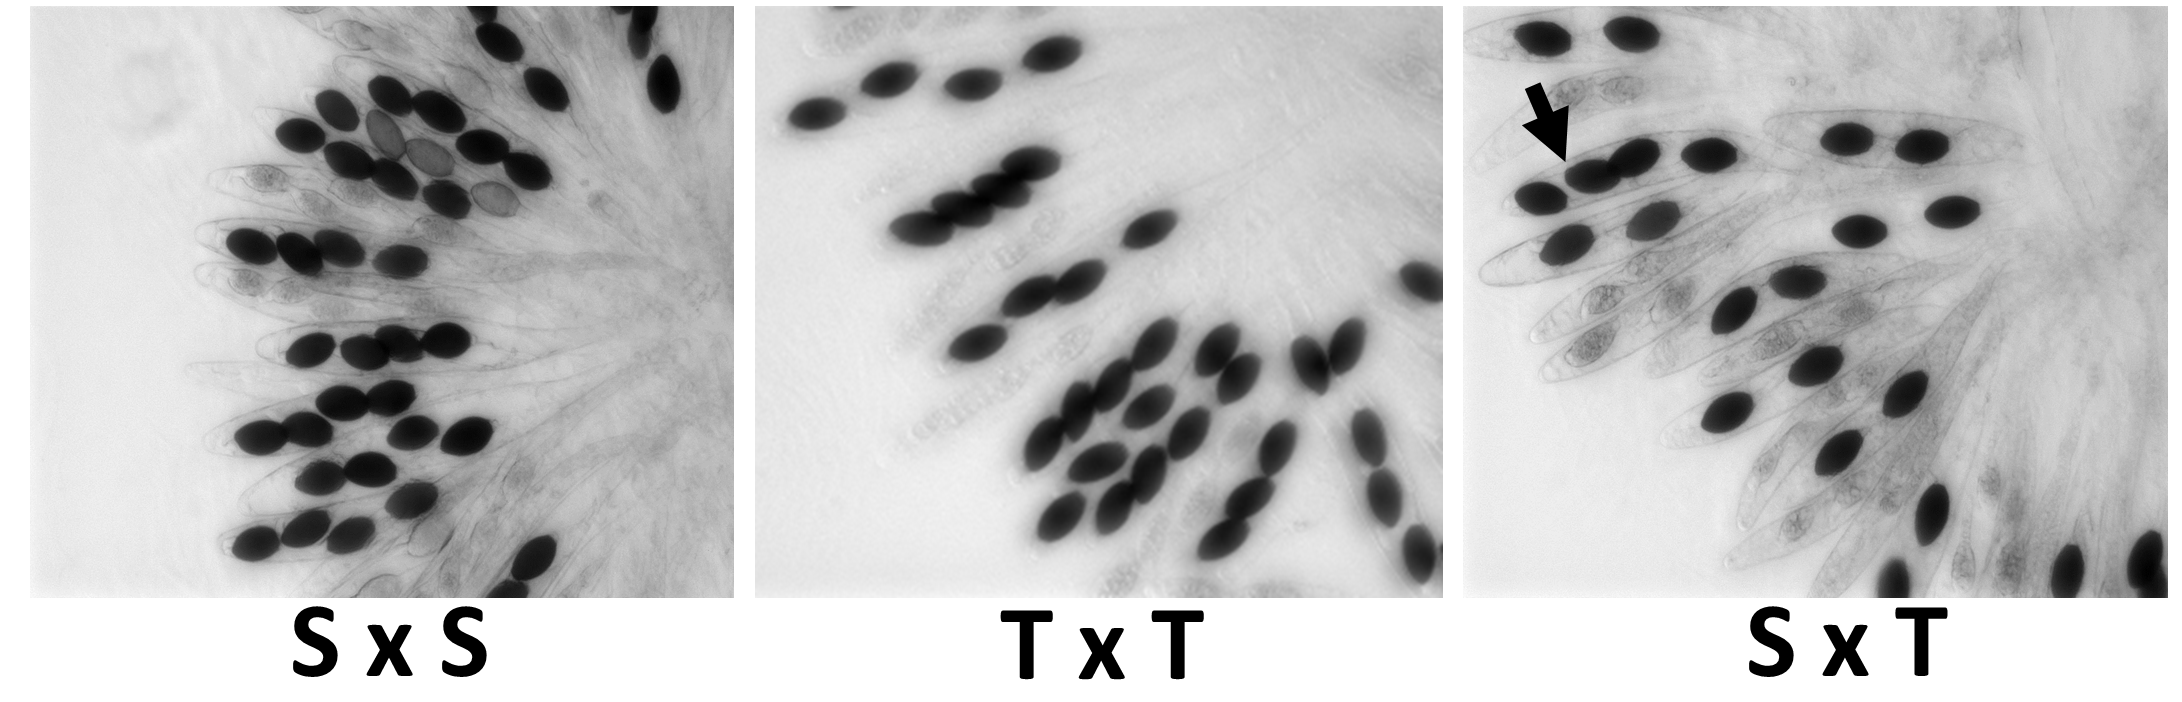
\includegraphics[width= \textwidth]{Journal_figs/single_locus_selection/ascus_spore_killer/Grognet_spore_killer.png}
\end{center}
\caption{
Pictures of {\it P. anserina} asci from various crosses. The arrow in the
SxT picture shows a rare  ascus carrying all four products of
meiosis. Figure from \citet{grognet2014genes}, \PLOSccBY. 
 } \label{fig:spore_killer}
\end{figure}
  

The four products of meiosis in the fungus {\it Podospora anserina}
are arrayed in the ascus\sidenote{from the Greek word askos meaning wineskin.}
of the spores for the next generation. There is a polymorphism S/T at
the Spok gene in this species. In
spores from SxS and TxT individuals all four products are
present. However, only two out of four spores are present in the
$\sim 90\%$ of asci from SxT individuals \citep{grognet2014genes}. The T allele is releasing
a toxin that poisons off the S carrying spores. The jury is still out
on whether the T allele spread due to the advantage created by
sabotaging its rival product of meiosis \citep{sweigart2019making}. However, in other systems it
is clear that alleles have spread due to their selfish actions. 

  \begin{figure}
\begin{center}
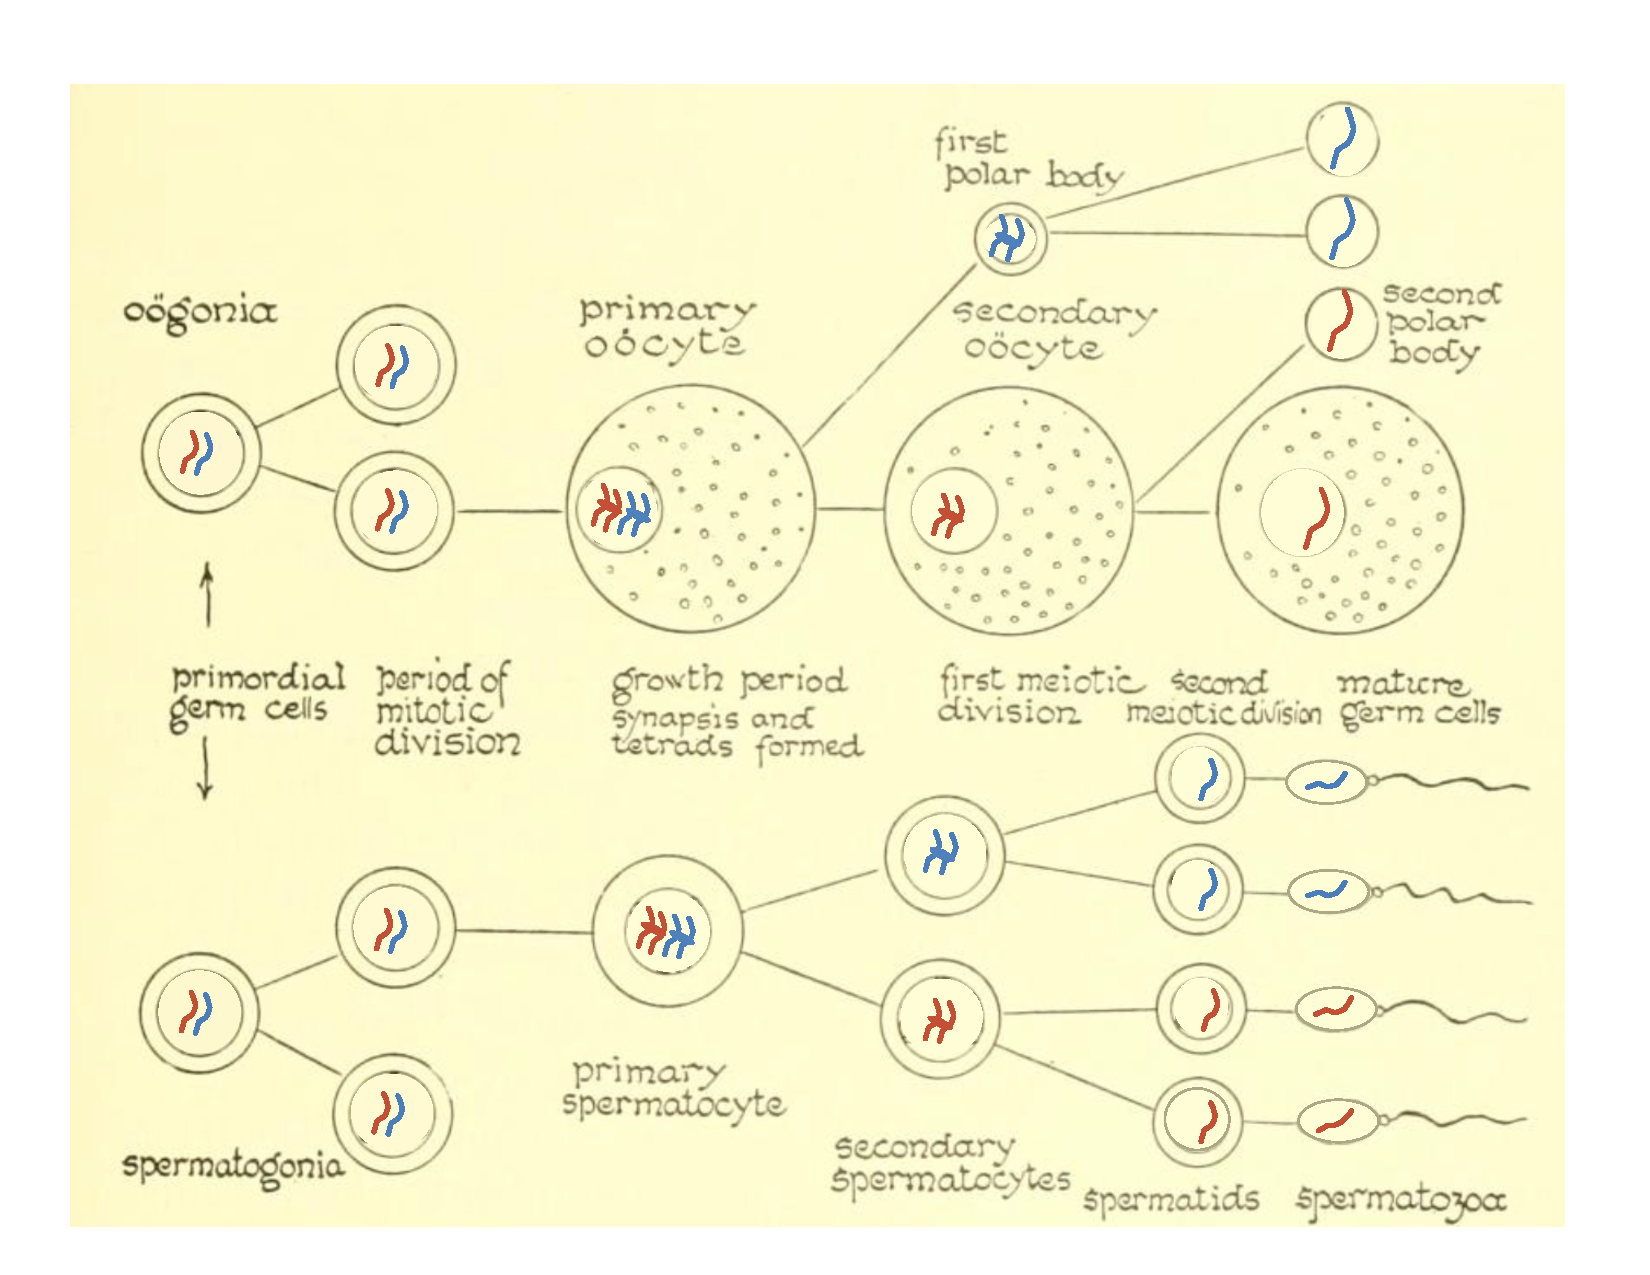
\includegraphics[width= \textwidth]{illustration_images/single_locus_selection/gametogenesis_male_female/gametogenesis_w_chr.pdf}
\end{center}
\caption{
   The two copies of a chromosome are shown in red and blue through
   the process of female and male meiosis and gametogenesis.  Crossovers are omitted to keep things simpler. 
Modified from original to include chromosomes transmitted.
  \BHLNKC{
Biology; the story of living things (1937).  Hunter, G.W., Walter
H.E.}{https://archive.org/stream/biologystoryofli00hunt/\#page/429/mode/1up}{MBLWHOI Library} } \label{fig:gametogenesis_male_female}
\end{figure}  % https://commons.wikimedia.org/wiki/File:Cramer%26Stoll-uitlandsche_kapellen_vol._1-_plate_065.jpg


A number of well-established genetics systems illustrate in
animals and plants how male and female gametogenesis offer different
opportunities for selfish alleles (Figure \ref{fig:gametogenesis_male_female}). Just as how selfish X chromosome systems can spread by
targeting sperm that carry the Y chromosome, selfish autosomal alleles
can spread by targeting sperm carrying the other chromosome in
heterozygotes. Both the Drosophila Segregation Distortion allele and
the mouse T-allele are selfish autosomal systems that
game transmission in heterozygotes by killing off sperm that don't carry the allele in heterozygotes.

%Spok asci killer system https://journals.plos.org/plosgenetics/article?id=10.1371/journal.pgen.1004387

In females meiosis there is a unique opportunity for cheating. In male
meiosis all four products of meiosis become gametes. 
However, only 1 of the four products of female meiosis becomes the egg, the other 3 products
are fated to become the polar bodies. Thus alleles can cheat in female meiosis by preferentially getting
transmitted into the egg rather than the polar body. If an allele on
a red chromosome (in top panel of Figure \ref{fig:gametogenesis_male_female}) can manipulate any asymmetry of meioses so that it can be
present in the egg $>50\%$ of the time it will have a transmission
advantage in female heterozygotes. 

 \begin{marginfigure}
\begin{center}
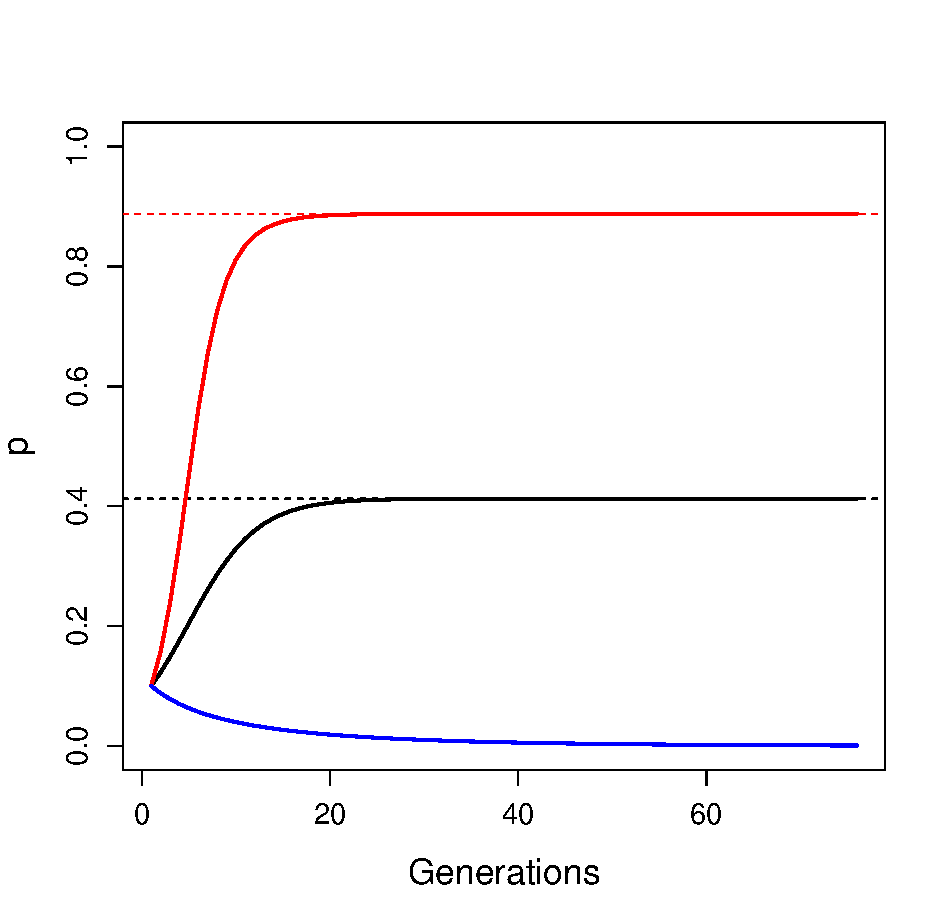
\includegraphics[width= \textwidth]{figures/autosomal_driver.pdf}
\end{center}
\caption{
The fate of an unfit transmission distorter allele. If transmission is
fair ($\alpha =\nicefrac
{1}{2}$, blue curve) the allele is lost, but the stronger its drive in
heterozygotes the faster its spread and the higher its final frequency
in the population (black and red curves, $\alpha =0.7$ \& $0.9$
respectively).  With fitnesses $w_{dd}=1$,
$w_{Dd}=0.95$, and $ w_{DD}=0.1$. The dotted lines show the predicted
equilibrium. 
  \gitcode{https://github.com/cooplab/popgen-notes/blob/master/Rcode/autosomal_driver.R}
} \label{fig:autosomal_driver}
\end{marginfigure} 


To see how such drivers can spread through the population lets
consider the case of a population where an allele drives in both male
and female gametogenesis. (Most selfish alleles will be sex-specific,
but that makes the math a little more tricky.)
Imagine a randomly-mating population of hermaphrodites. In this
population, a derived allele (D) segregates that distorts transmission
in its favour over the ancestral allele (d) in the production of all
the gametes of heterozygotes. The drive leads to a fraction $\alpha$ of the gametes
of heterozygotes (D/d) to carry the D allele ($\alpha \geq 0.5$). The D allele
causes viability problems such that the
relative fitnesses are $w_{dd}=1$, $1 > w_{Dd} \geq w_{DD}$. If the D allele
is currently at frequency p in the population at birth, its frequency
at birth in the next generation will be
\begin{equation}
p^{\prime}=\frac{w_{DD}p^2 + w_{Dd} \alpha 2pq  }{\wbar} \label{eq:auto_driver}
 \end{equation}
when $\alpha=\nicefrac{1}{2}$, i.e. fair Mendelian transmission this is exactly the same as our directional selection, which results in our $D$
allele being selected out of the population (blue line, Figure \ref{fig:autosomal_driver}). However, if
$\alpha>\nicefrac{1}{2}$, i.e. our deleterious allele cheats, it can potentially
increase in the population when it is rare (red and black lines,
Figure \ref{fig:autosomal_driver})). However, the allele can become
trapped in the population at a polymorphic equilibrium if its cost is
sufficient in homozygotes. This is akin to the case of heterozygote
advantage, but now our allele offers no advantage to heterozygote but
has a self advantage in heterozygotes.

\begin{question} (Tricker question)
  With reference to of our autosomal driver from equation
  \ref{eq:auto_driver}.\\
  {\bf A)}	Imagine the cost of the driver were additive, i.e.  $w_{dd}=1$, $w_{Dd}=1-e$, $w_{DD}=1-2e$. Under what conditions can the
driver invade the population? Can a polymorphic equilibrium be maintained?\\
{\bf B)}	Imagine the allele is completely recessive, i.e. $w_{dd}=w_{Dd}=1$. What conditions do you need for a polymorphic equilibrium to be maintained? What is the equilibrium frequency of this balanced polymorphism?\\
\end{question}

Many of the known autosomal drive systems are polymorphic in
populations, unable to reach fixation in the population due to their
costs in homozygotes. It seems likely that this represents an
ascertainment bias, and that many other selfish systems that had
lower selective costs have swept to
fixation. 
%mother's curse in people
% https://www.theatlantic.com/science/archive/2017/09/how-a-fille-du-roy-brought-the-mothers-curse-to-canada/540153/

% sperm and egg production https://www.biodiversitylibrary.org/ia/cu31924001006851#page/60/mode/1up
% https://archive.org/stream/embryologyofinse00joha/#page/4/mode/1up
% BEST ONE https://archive.org/stream/biologystoryofli00hunt/#page/429/mode/1up

\subsection{Appendix: ESS for the sex ratio} \label{ESS_sex_Ratio}
Let $R$ be the resources available to an individuals and $C_{\mars}$ and $C_{\venus}$ be the cost of
producing a son and daughter respectively. If our focal mother directs
$s$ of her effort towards sons and $(1-s)$ of her effort towards
daughters, she'll produce $\frac{Rs}{C_{\mars}}$ sons and
$\frac{R(1-s)}{C_{\venus}}$ daughters.  Let's assume that the mean
reproductive value of daughters is $1$. Given this, the average reproductive
value of sons is the average number of matings that a male will have,
i.e. the ratio $\nicefrac{\# \textrm{~females}}{\# \textrm{~males}}$. So if the population has a sex ratio $s_p$, the fitness of our focal female is
\begin{equation}
W(s,s_p) = \left( \frac{R(1-s)}{C_{\venus}} \times 1 \right) +  \left( \frac{Rs}{C_{\mars}} \times  \frac{\nicefrac{R(1-s_p)}{C_{\venus}} }{\nicefrac{Rs_p}{C_{\mars}}} \right) \label{sex_ratio_focal}
\end{equation}
expressing fitness in terms the number of grandkids our focal female is expected to have.

To find the ESS we want a sex ratio $s^*$ for the population such that
no mutant has higher fitness. We can write this as as the population
having strategy $s_p=s^*$, and then seeing what choice of $s^*$ leads
to $W(s^*,s^*)> W(s,s^*)$ for $s \neq s^*$, i.e. that no new
strategy ($s$) has higher fitness than the ESS strategy $s*$. We can
find this ESS $s^*$ by
\begin{equation}
\left. \frac{\partial W(s,s_p)}{\partial s} \right\vert_{s^* = s=s_p} = 0
\end{equation}
taking the derivative of Eqn \ref{sex_ratio_focal} we obtain
\begin{equation}
\frac{\partial W(s,s_p)}{\partial s}  = - \frac{R}{C_{\venus}} +  \frac{R}{C_{\mars}} \left( \frac{\nicefrac{R(1-s_p)}{C_{\venus}} }{\nicefrac{Rs_p}{C_{\mars}}} \right) 
\end{equation}
setting $s^* = s=s_p$ and rearranging
\begin{equation}
\frac{R}{C_{\venus}} =  \frac{R}{C_{\mars}} \left( \frac{\nicefrac{R(1-s^*)}{C_{\venus}} }{\nicefrac{Rs^*}{C_{\mars}}} \right) 
\end{equation}
which is satisfied when $s^* = \nicefrac{1}{2}$, i.e. devoting equal resources to male and female offspring is the ESS, which corresponds to a 50/50 sex ratio if male and female offspring are equally costly. 

